\section{Analysis of the \texorpdfstring{\ttH}{ttH} mode}
\label{sec:htoinv_analysis_ttH}

The fit of signal and background to the observed data is performed for each subcategory of \ttH, in addition to the category as a whole.\footnote{Might make more sense to have a section called ``Results'', and then these ``Analysis of the X mode'' and combined results as subsections.} Due to limited statistical precision, the dilepton \glspl{CR} in the boosted subcategories are combined into a single bin, i.e., inclusive of both subcategory and \ptmiss. The rate parameter for the prediction of the \ztonunu background in the signal region is therefore a single value shared across the boosted subcategories and their \ptmiss bins. The \singlePhotonCr \gls{CR} is not used in constraining the \ztonunu prediction for any of the subcategories.

To predict the \acrshort{qcd} event counts in the signal region, Eq.~\ref{eq:qcd_prediction} incorporates the \acrshort{mc} counts in said region and from one or more sidebands. The tight double sideband from Tab.~\ref{tab:sideband_defs}---the most enriched in multijet \acrshort{mc}---is employed to derive the category fraction \catFraction. Yields from the loose double sideband compute the remaining terms: the \ptmiss fraction \metFraction, $N_{\mathrm{SB}}^{\mathrm{QCD}}$, and $\transfac_{\mathrm{QCD}}$.

Results are presented in terms of the upper limit on the signal strength parameter $\sigma \times \BRof{\higgstoinv} / \sigma_{\mathrm{SM}}$. The observed limit in the signal plus background hypothesis at 95\,\% confidence level is overlaid on the expectation from the background-only hypothesis. In the latter, the median expected limit is illustrated with accompanying boundaries for its 1$\sigma$ and 2$\sigma$ deviations. Fig.~\ref{fig:htoinv_limit_ttH} showcases the limits for each \ttH subcategory and the combination of them all, for each data taking year individually and over the full Run-2 dataset.

\begin{figure}[htbp]
    \centering
    \begin{subfigure}[b]{0.45\textwidth}
        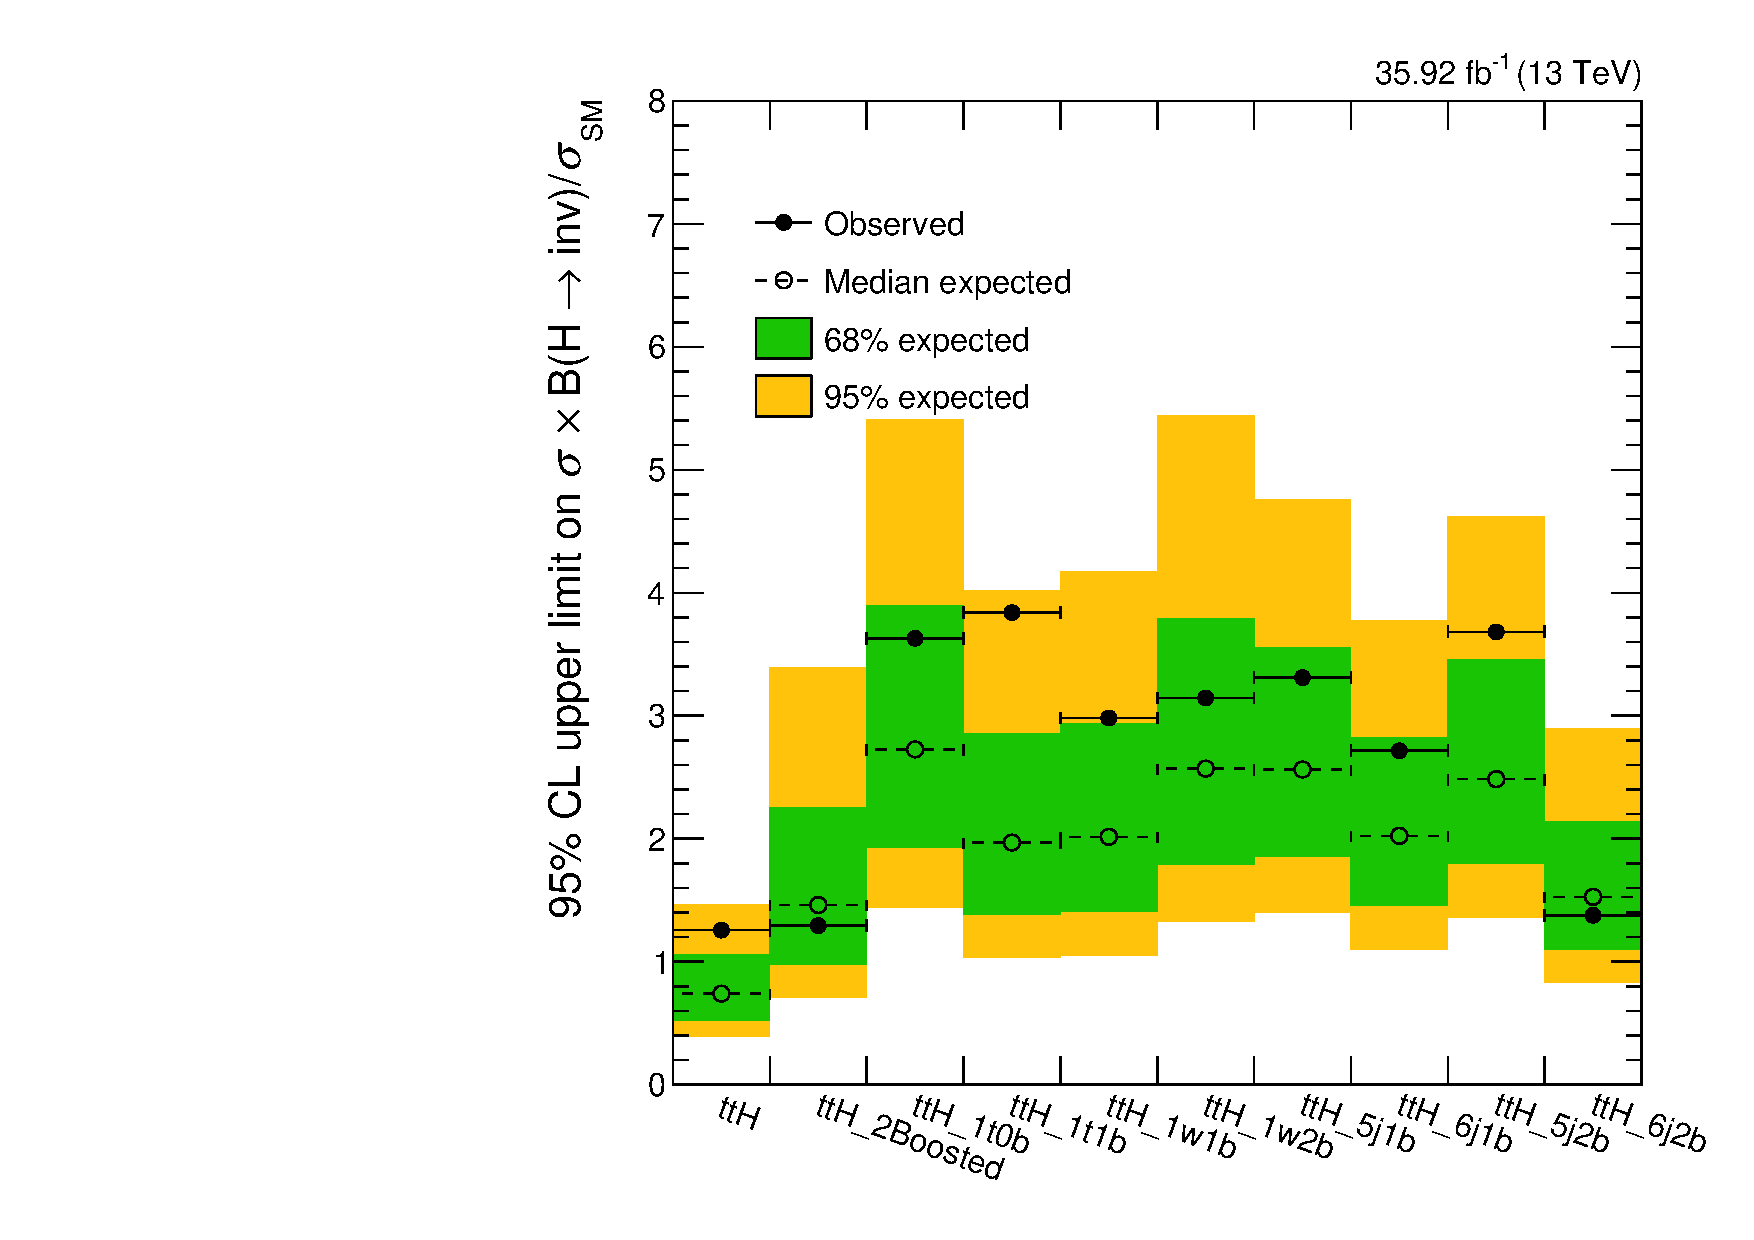
\includegraphics[width=\textwidth]{figures/limits/ttH/limit_2016_ttH.pdf}
        \caption{\ttH --- 2016}
    \end{subfigure}
    \hfill
    \begin{subfigure}[b]{0.45\textwidth}
        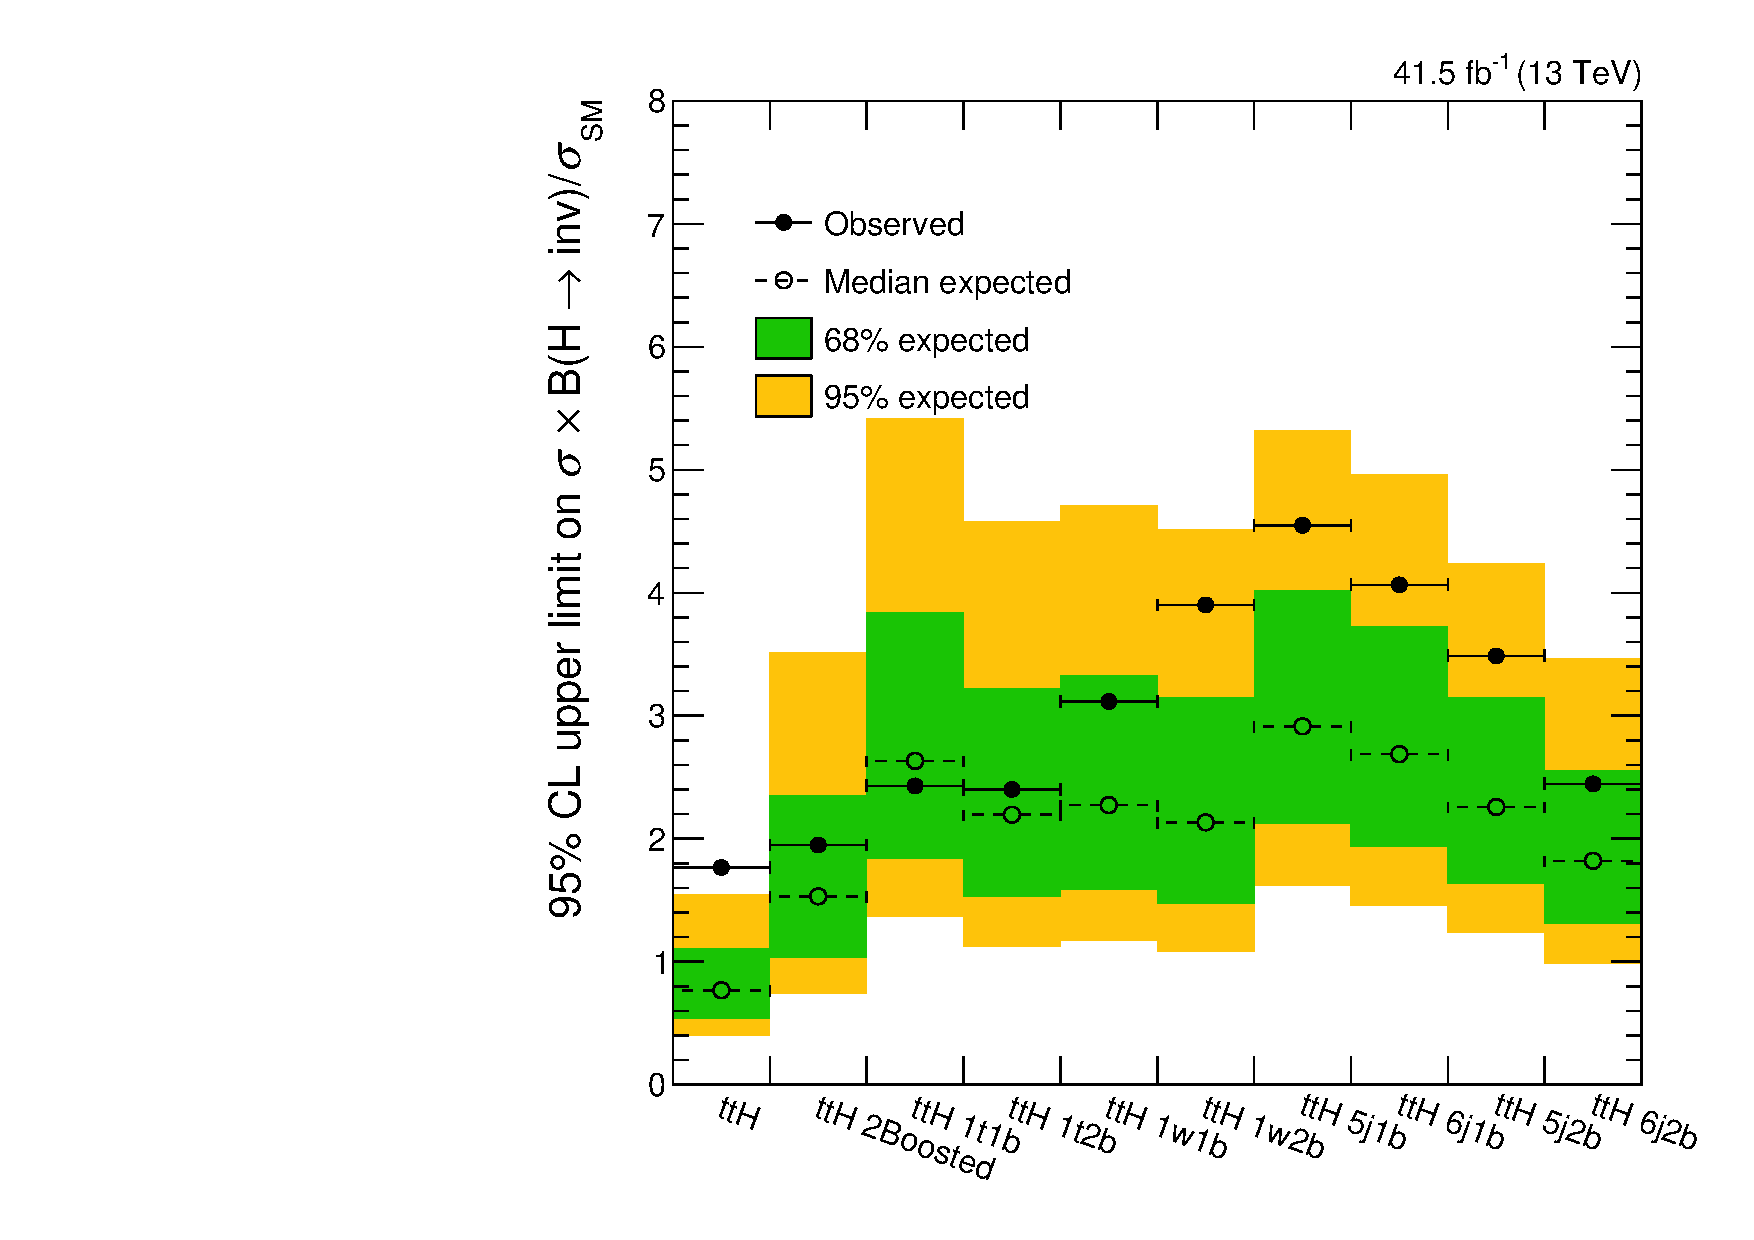
\includegraphics[width=\textwidth]{figures/limits/ttH/limit_2017_ttH.pdf}
        \caption{\ttH --- 2017}
    \end{subfigure}

    \begin{subfigure}[b]{0.45\textwidth}
        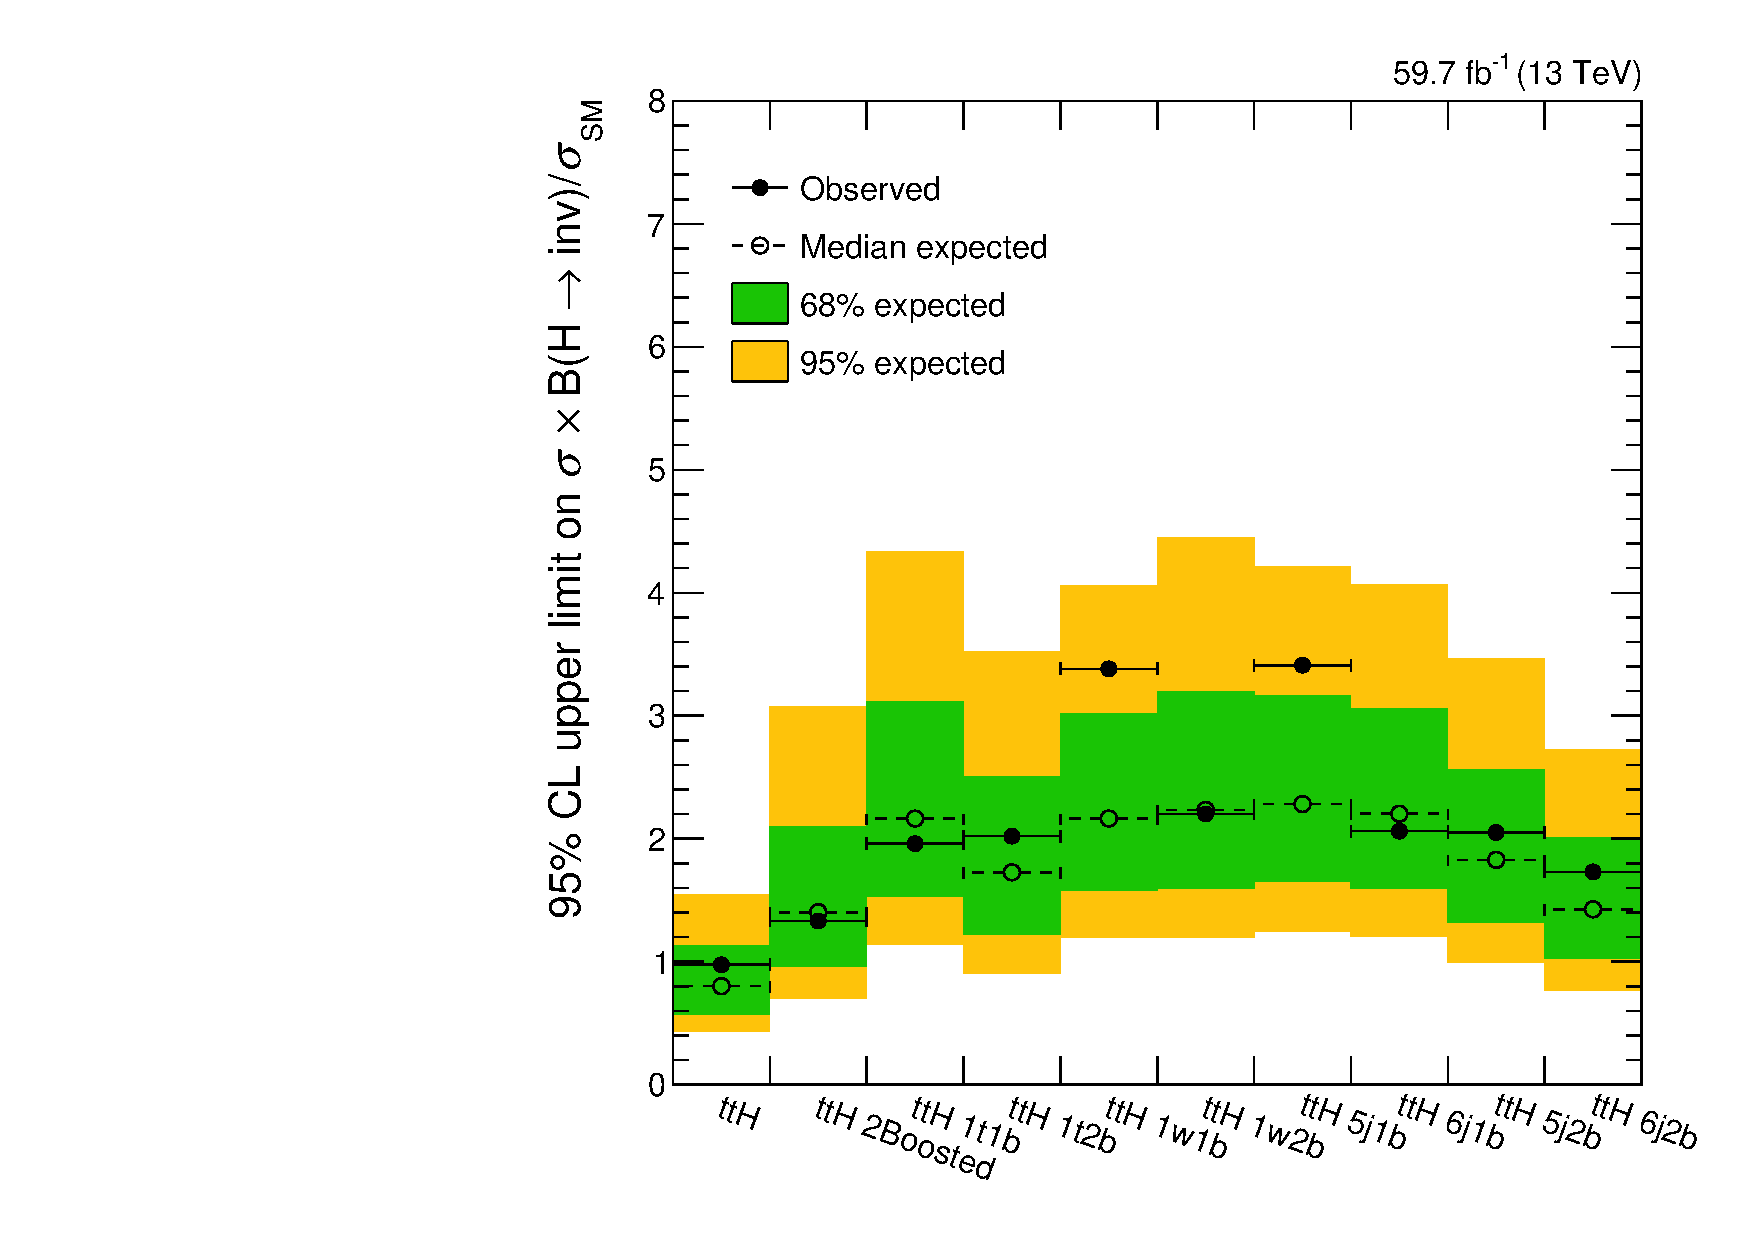
\includegraphics[width=\textwidth]{figures/limits/ttH/limit_2018_ttH.pdf}
        \caption{\ttH --- 2018}
    \end{subfigure}
    \hfill
    \begin{subfigure}[b]{0.45\textwidth}
        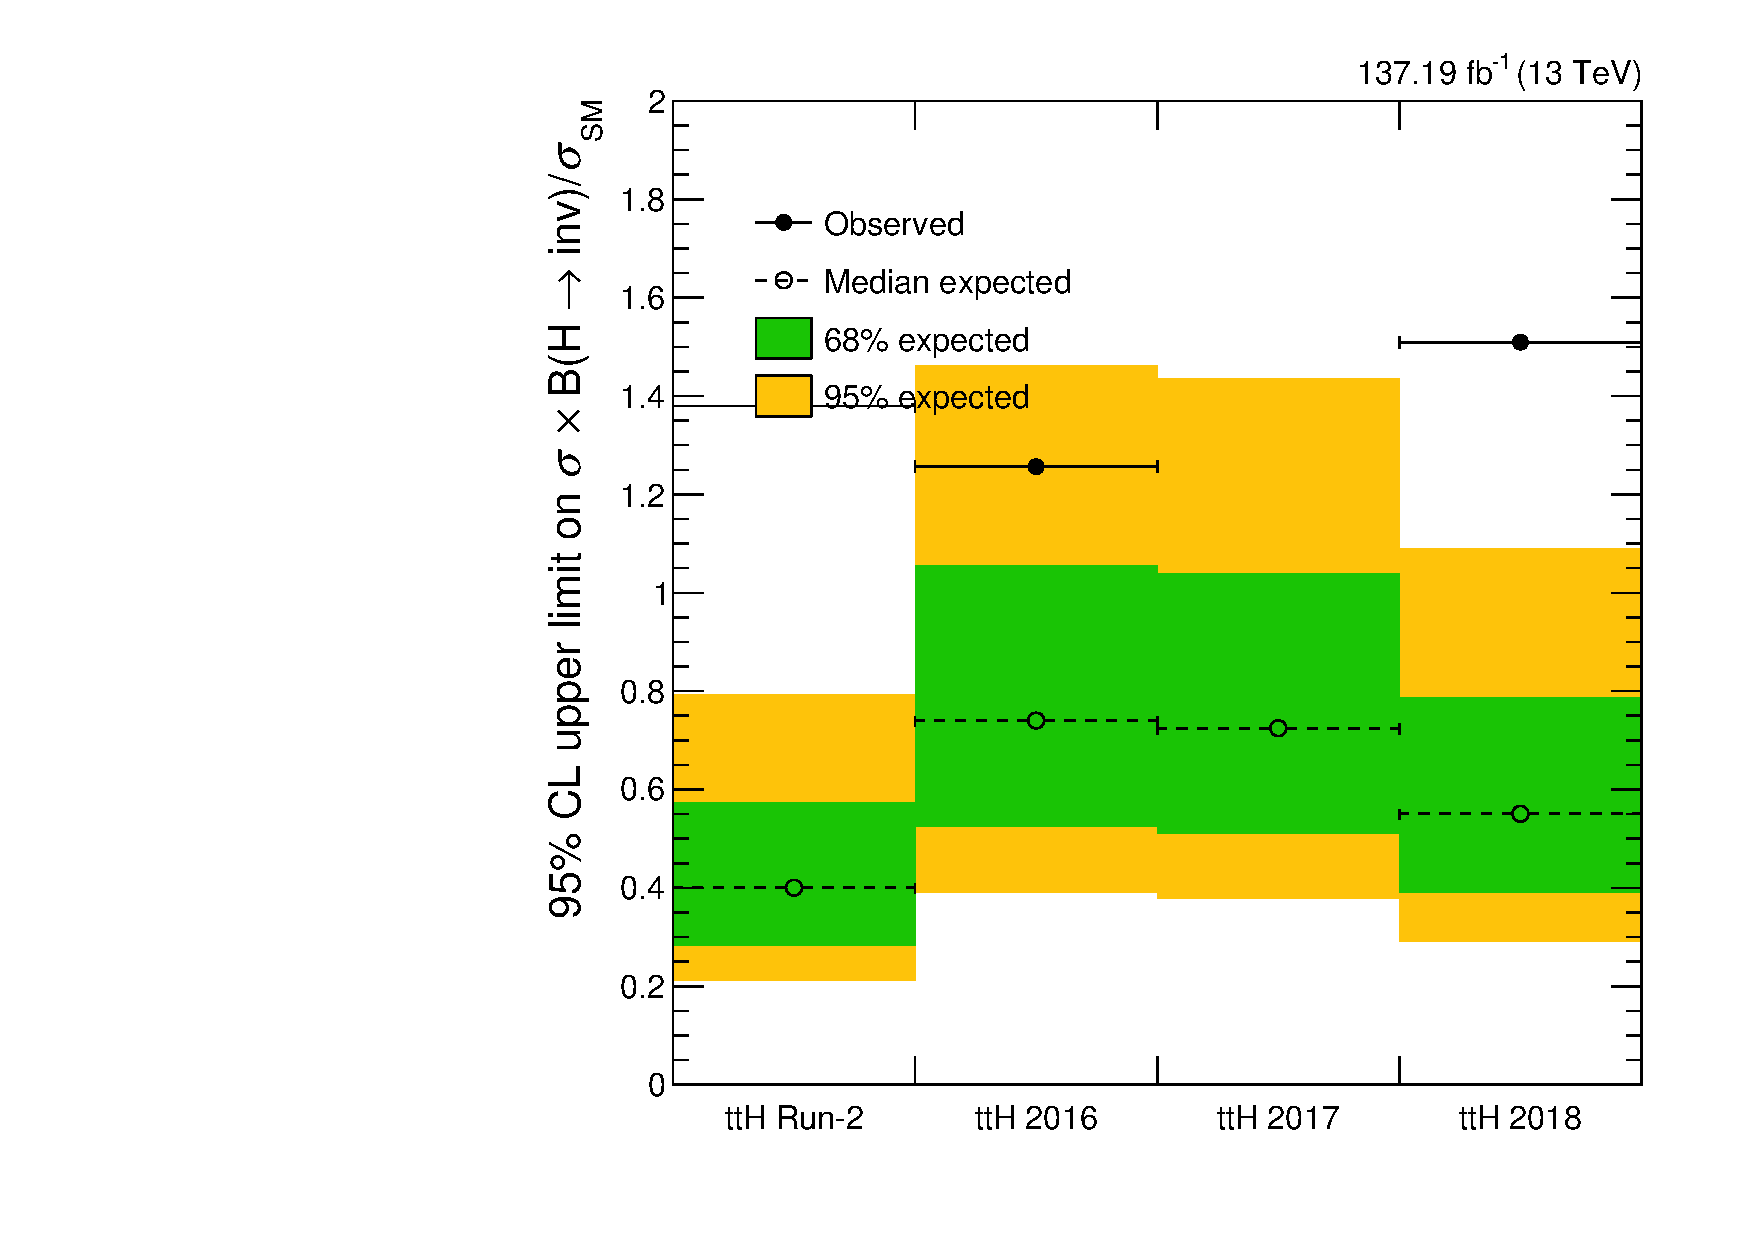
\includegraphics[width=\textwidth]{figures/limits/ttH/limit_Run2_ttH.pdf}
        \caption{\ttH --- Run-2}
    \end{subfigure}
    \caption[Observed and expected 95\,\% CL upper limits on the Higgs boson to invisible state branching fraction in the \ttH category, for both the individual subcategories, and the combination of them, for each data-taking year in Run-2]{Observed and expected 95\,\% CL upper limits on the Higgs boson to invisible state branching fraction in the \ttH category, for both the individual subcategories, and the combination of them, for each data-taking year in Run-2.}
    \label{fig:htoinv_limit_ttH}
\end{figure}

Distributions of the pre-fit and post-fit yields for 2016, 2017, and 2018 are displayed in Figs.~\ref{fig:htoinv_mountain_range_ttH_2016}, \ref{fig:htoinv_mountain_range_ttH_2017}, and \ref{fig:htoinv_mountain_range_ttH_2018}, respectively.\footnote{Not showing control regions as it's probably an overload. Also might be worth moving to an appendix or something. Will try to add pre-fit and post-fit on the same plot to halve the number of them.}

\begin{figure}[htbp]
    \centering
    \begin{subfigure}[b]{0.9\textwidth}
        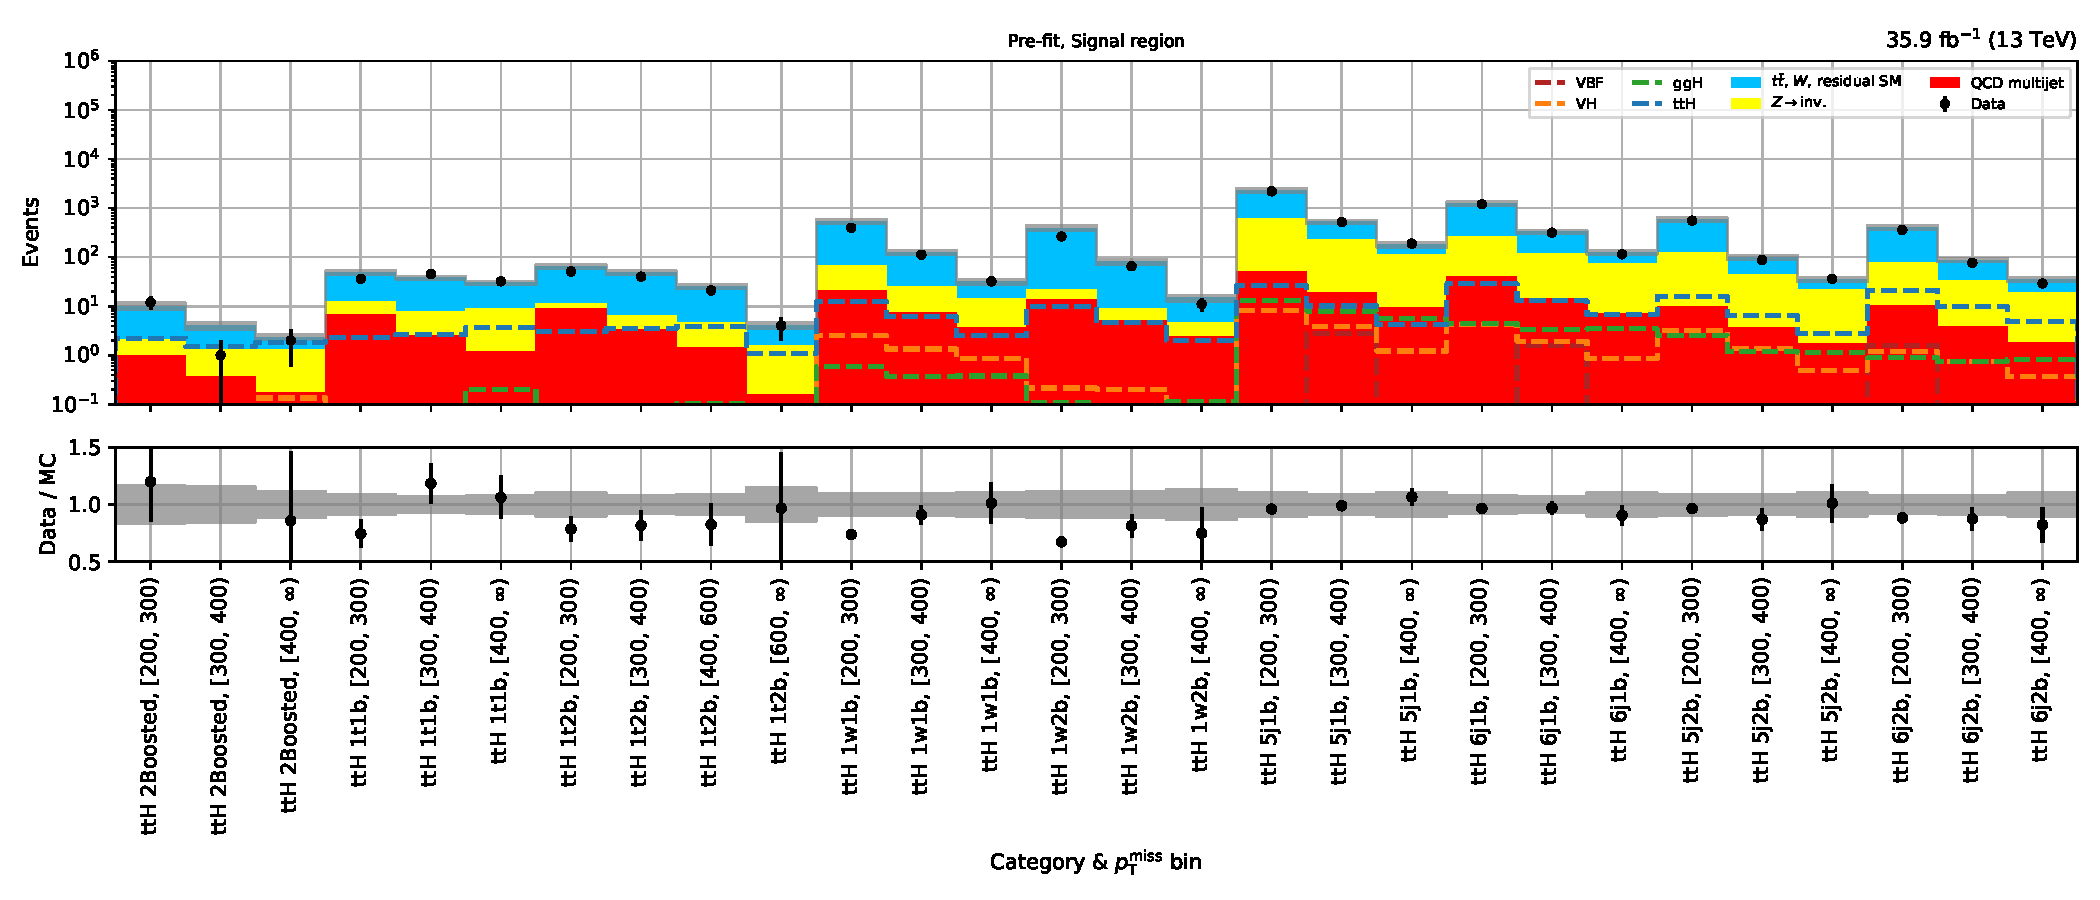
\includegraphics[width=\textwidth]{figures/mountain_ranges/2016/ttH/SR_tree_prefit-abs_values_ttH_cats.pdf}
        \caption{\ttH --- 2016 (pre-fit)}
    \end{subfigure}

    \begin{subfigure}[b]{0.9\textwidth}
        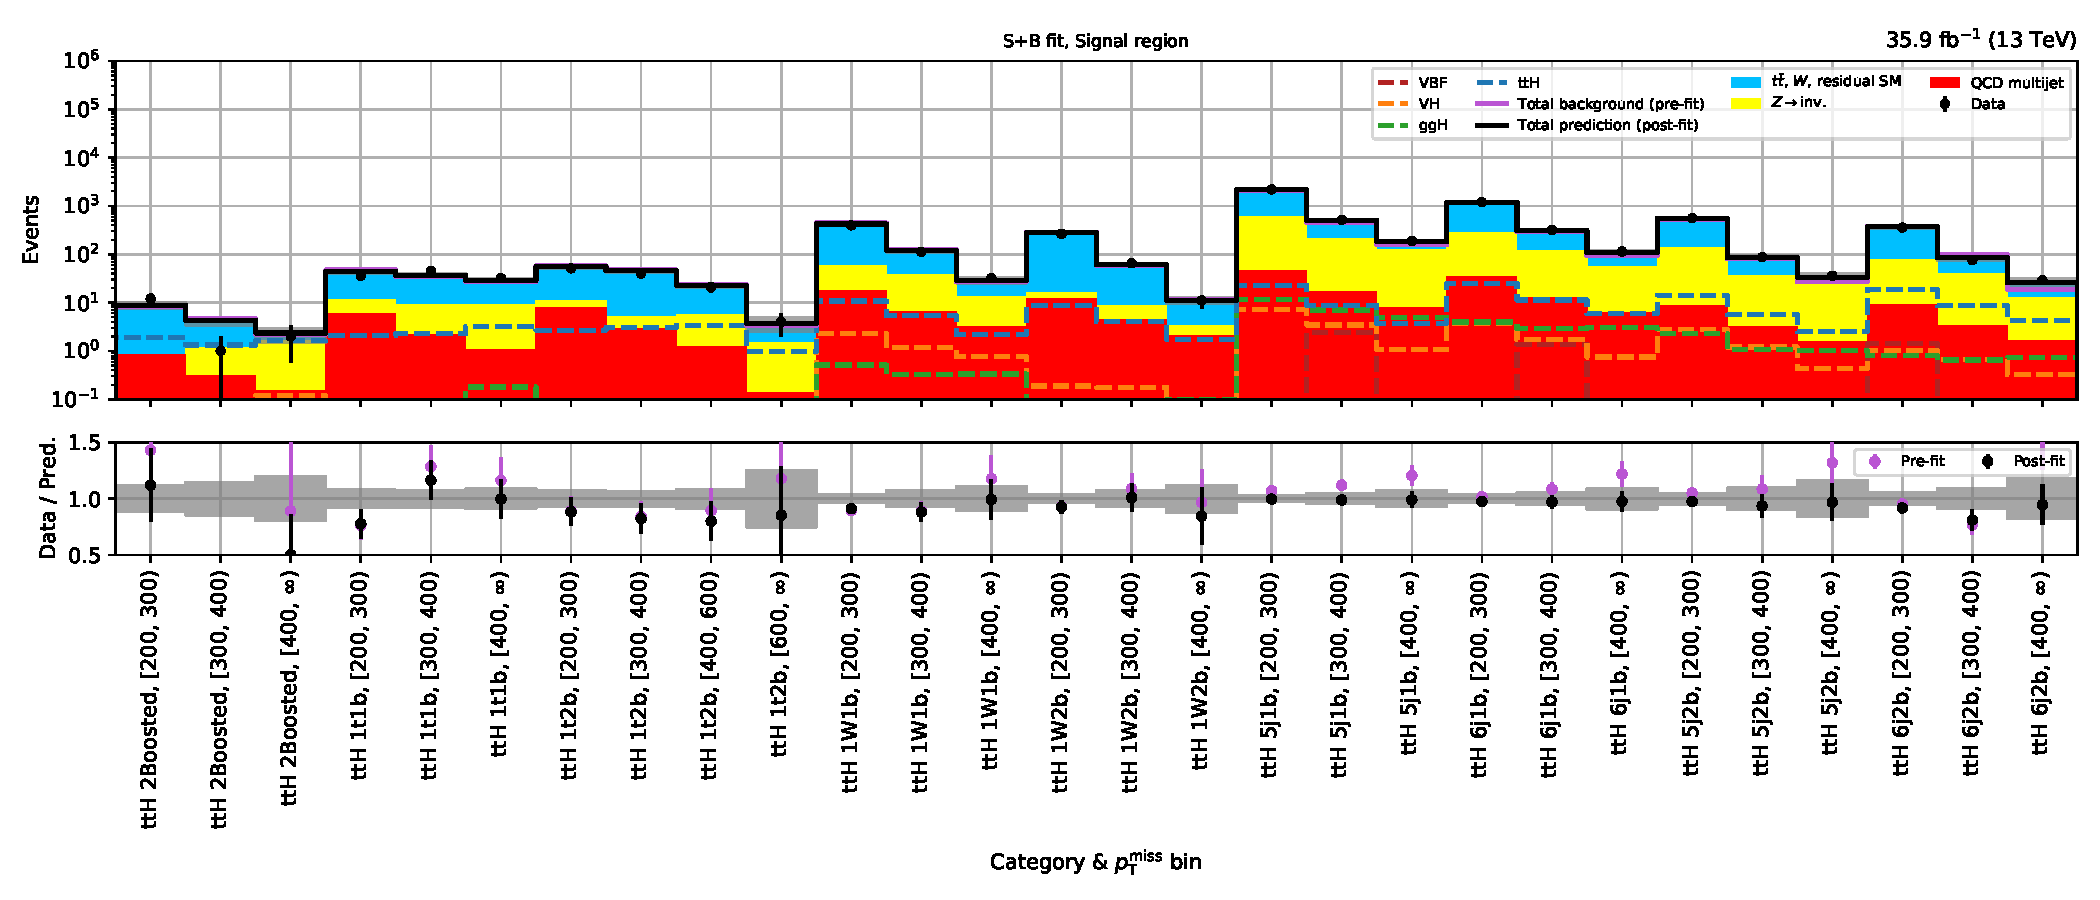
\includegraphics[width=\textwidth]{figures/mountain_ranges/2016/ttH/SR_tree_fit_s-abs_values_ttH_cats.pdf}
        \caption{\ttH --- 2016 (post-fit)}
    \end{subfigure}
    \caption[Pre-fit and post-fit yields for each \ttH subcategory and \ptmiss bin for the 2016 dataset]{Pre-fit and post-fit yields for each \ttH subcategory and \ptmiss bin for the 2016 dataset. In bottom panel of post-fit plot, the ratio data to signal plus background is calculated.}
    \label{fig:htoinv_mountain_range_ttH_2016}
\end{figure}

\begin{figure}[htbp]
    \centering
    \begin{subfigure}[b]{0.9\textwidth}
        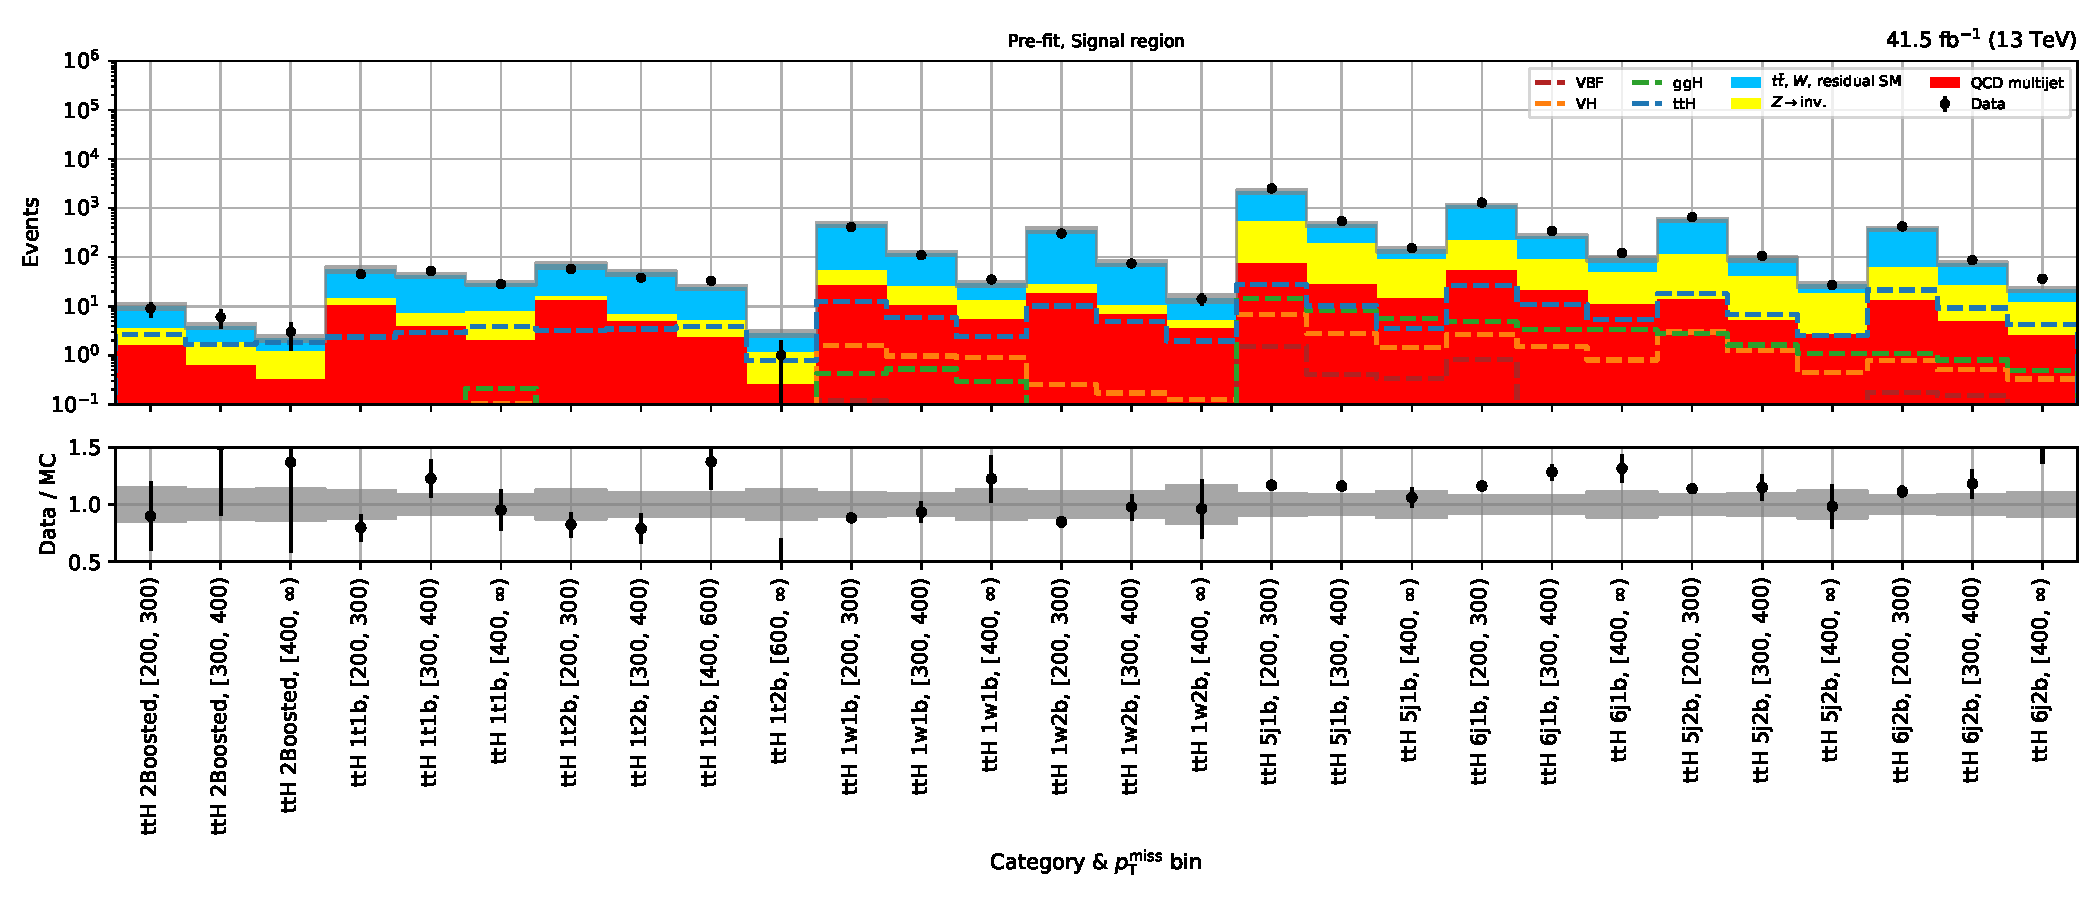
\includegraphics[width=\textwidth]{figures/mountain_ranges/2017/ttH/SR_tree_prefit-abs_values_ttH_cats.pdf}
        \caption{\ttH --- 2017 (pre-fit)}
    \end{subfigure}

    \begin{subfigure}[b]{0.9\textwidth}
        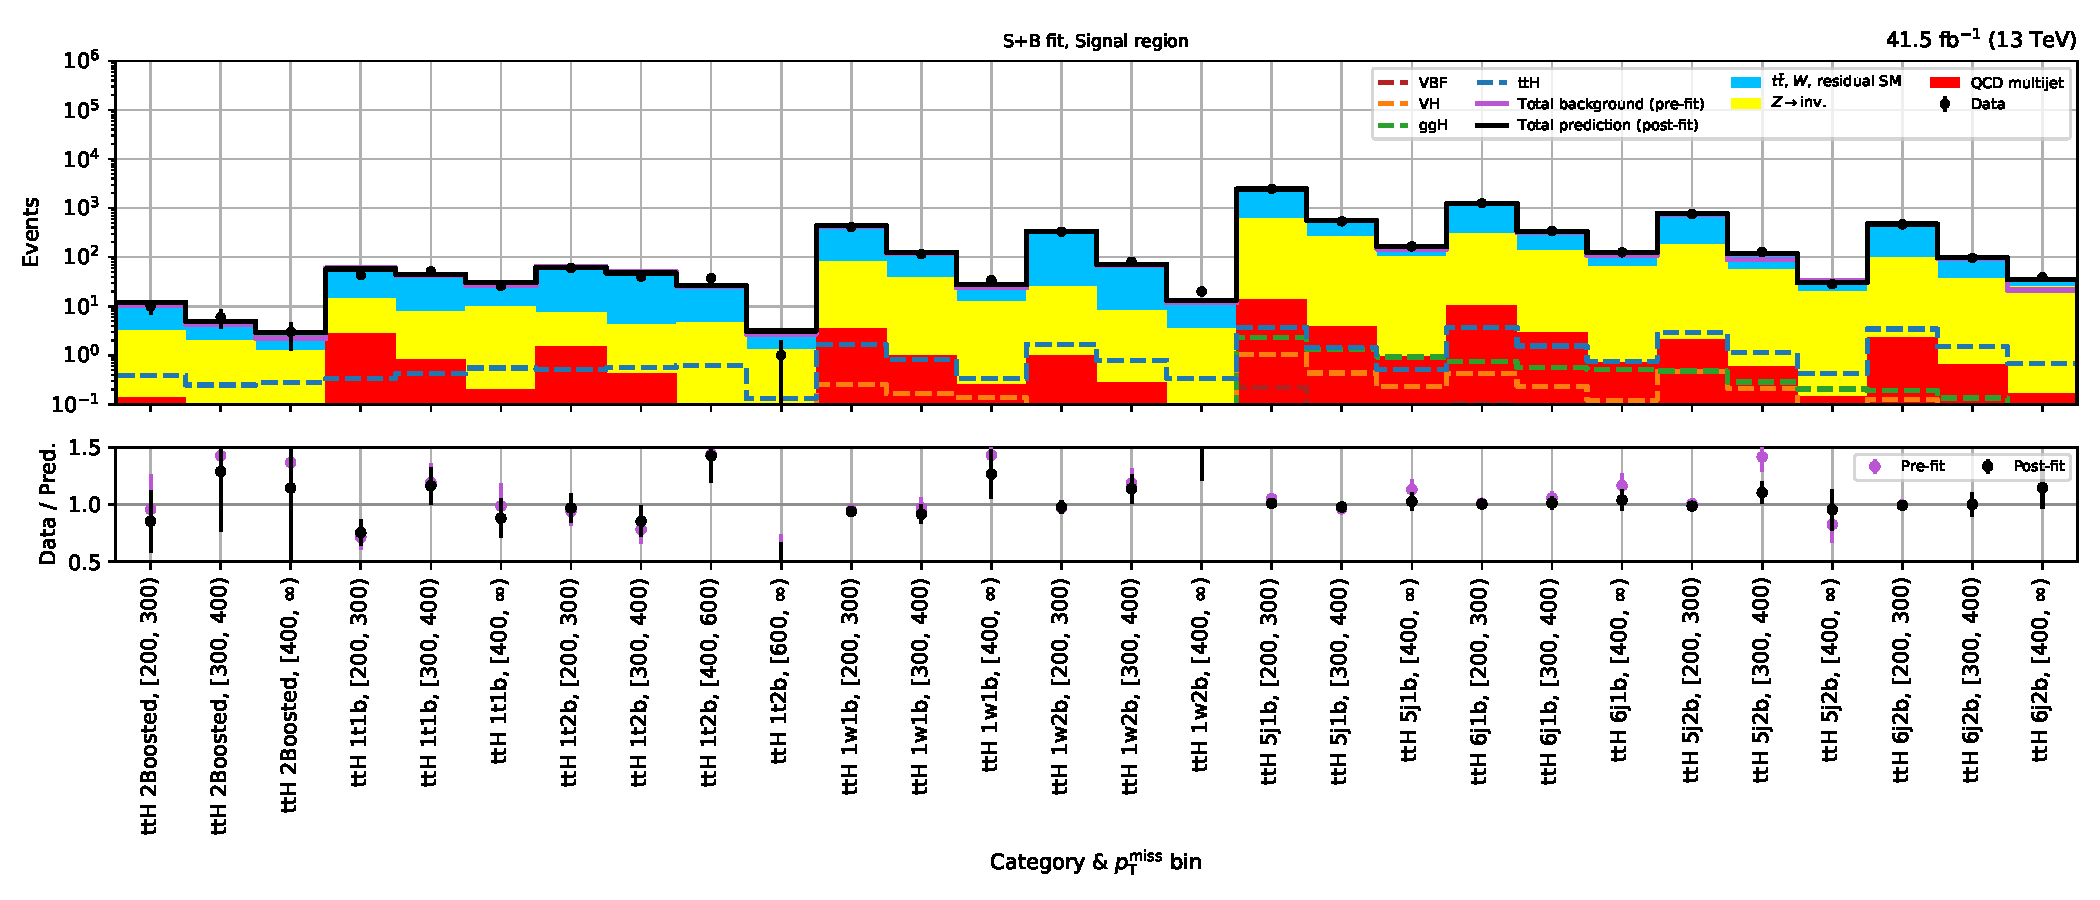
\includegraphics[width=\textwidth]{figures/mountain_ranges/2017/ttH/SR_tree_fit_s-abs_values_ttH_cats.pdf}
        \caption{\ttH --- 2017 (post-fit)}
    \end{subfigure}
    \caption[Pre-fit and post-fit yields for each \ttH subcategory and \ptmiss bin for the 2017 dataset]{Pre-fit and post-fit yields for each \ttH subcategory and \ptmiss bin for the 2017 dataset. In bottom panel of post-fit plot, the ratio data to signal plus background is calculated.}
    \label{fig:htoinv_mountain_range_ttH_2017}
\end{figure}

\begin{figure}[htbp]
    \centering
    \begin{subfigure}[b]{0.9\textwidth}
        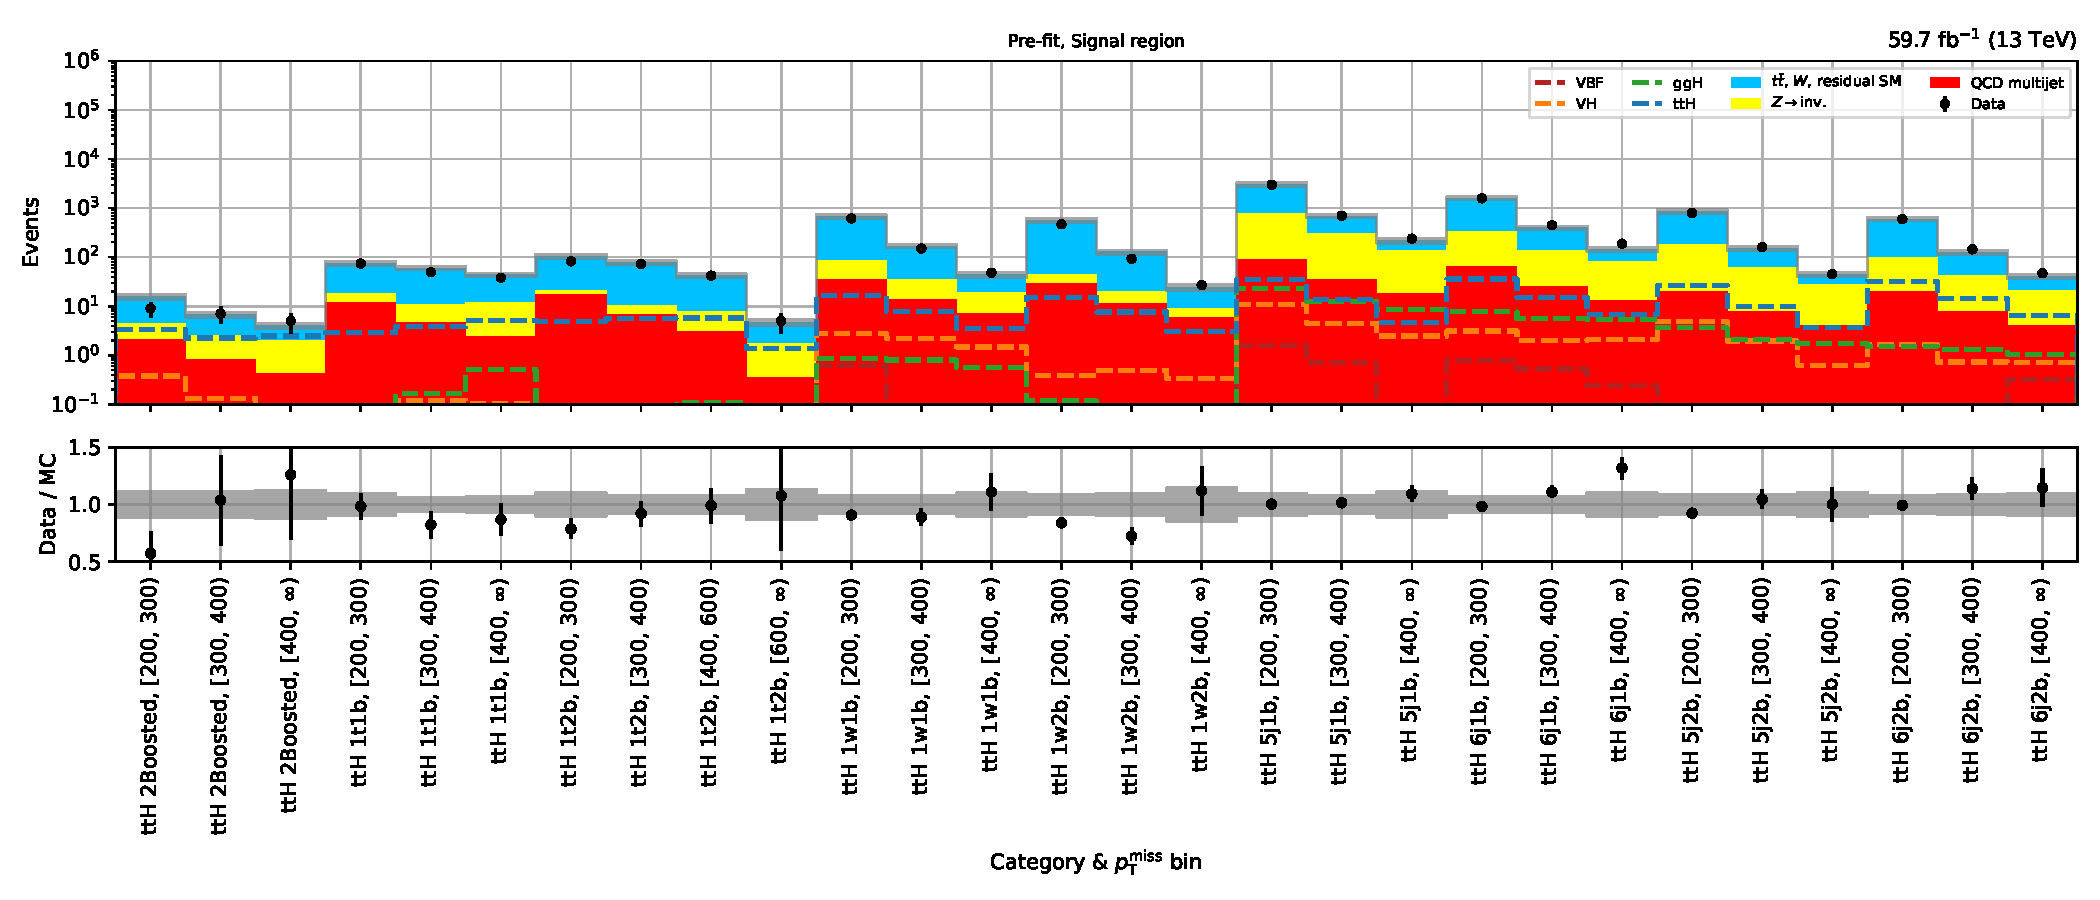
\includegraphics[width=\textwidth]{figures/mountain_ranges/2018/ttH/SR_tree_prefit-abs_values_ttH_cats.pdf}
        \caption{\ttH --- 2018 (pre-fit)}
    \end{subfigure}

    \begin{subfigure}[b]{0.9\textwidth}
        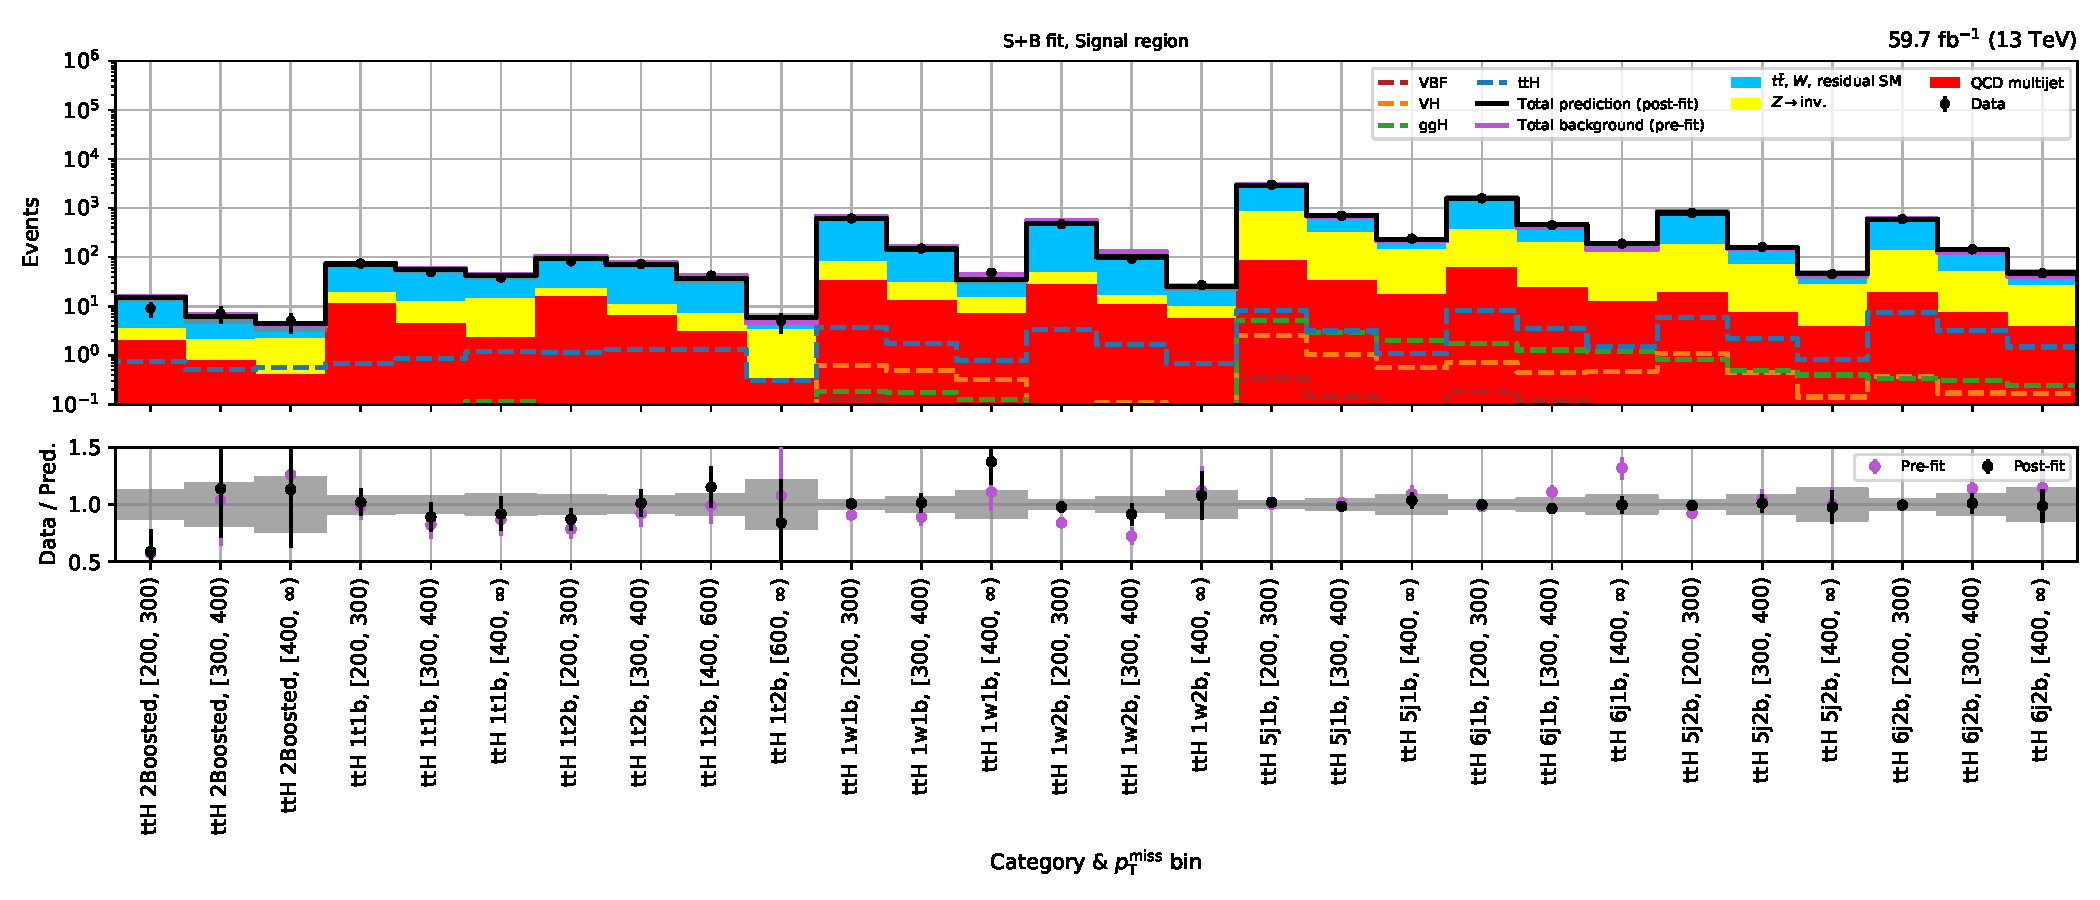
\includegraphics[width=\textwidth]{figures/mountain_ranges/2018/ttH/SR_tree_fit_s-abs_values_ttH_cats.pdf}
        \caption{\ttH --- 2018 (post-fit)}
    \end{subfigure}
    \caption[Pre-fit and post-fit yields for each \ttH subcategory and \ptmiss bin for the 2018 dataset]{Pre-fit and post-fit yields for each \ttH subcategory and \ptmiss bin for the 2018 dataset. In bottom panel of post-fit plot, the ratio data to signal plus background is calculated.}
    \label{fig:htoinv_mountain_range_ttH_2018}
\end{figure}

\clearpage


%=========================================================


\section{Analysis of the \texorpdfstring{\VH}{VH} mode}
\label{sec:htoinv_analysis_VH}

Contrary to \ttH, all of the \glspl{CR} are utilised in the non-multijet background predictions with a fully granular correspondence to the signal region.\footnote{Add a sentence or two about how QCD prediction is done. Might be different from ttH.}

Fig.~\ref{fig:htoinv_limit_VH} showcases the expected and observed limits for the \VH subcategories and their combination for each data taking year as well the result for the full Run-2 dataset.

\begin{figure}[htbp]
    \centering
    \begin{subfigure}[b]{0.45\textwidth}
        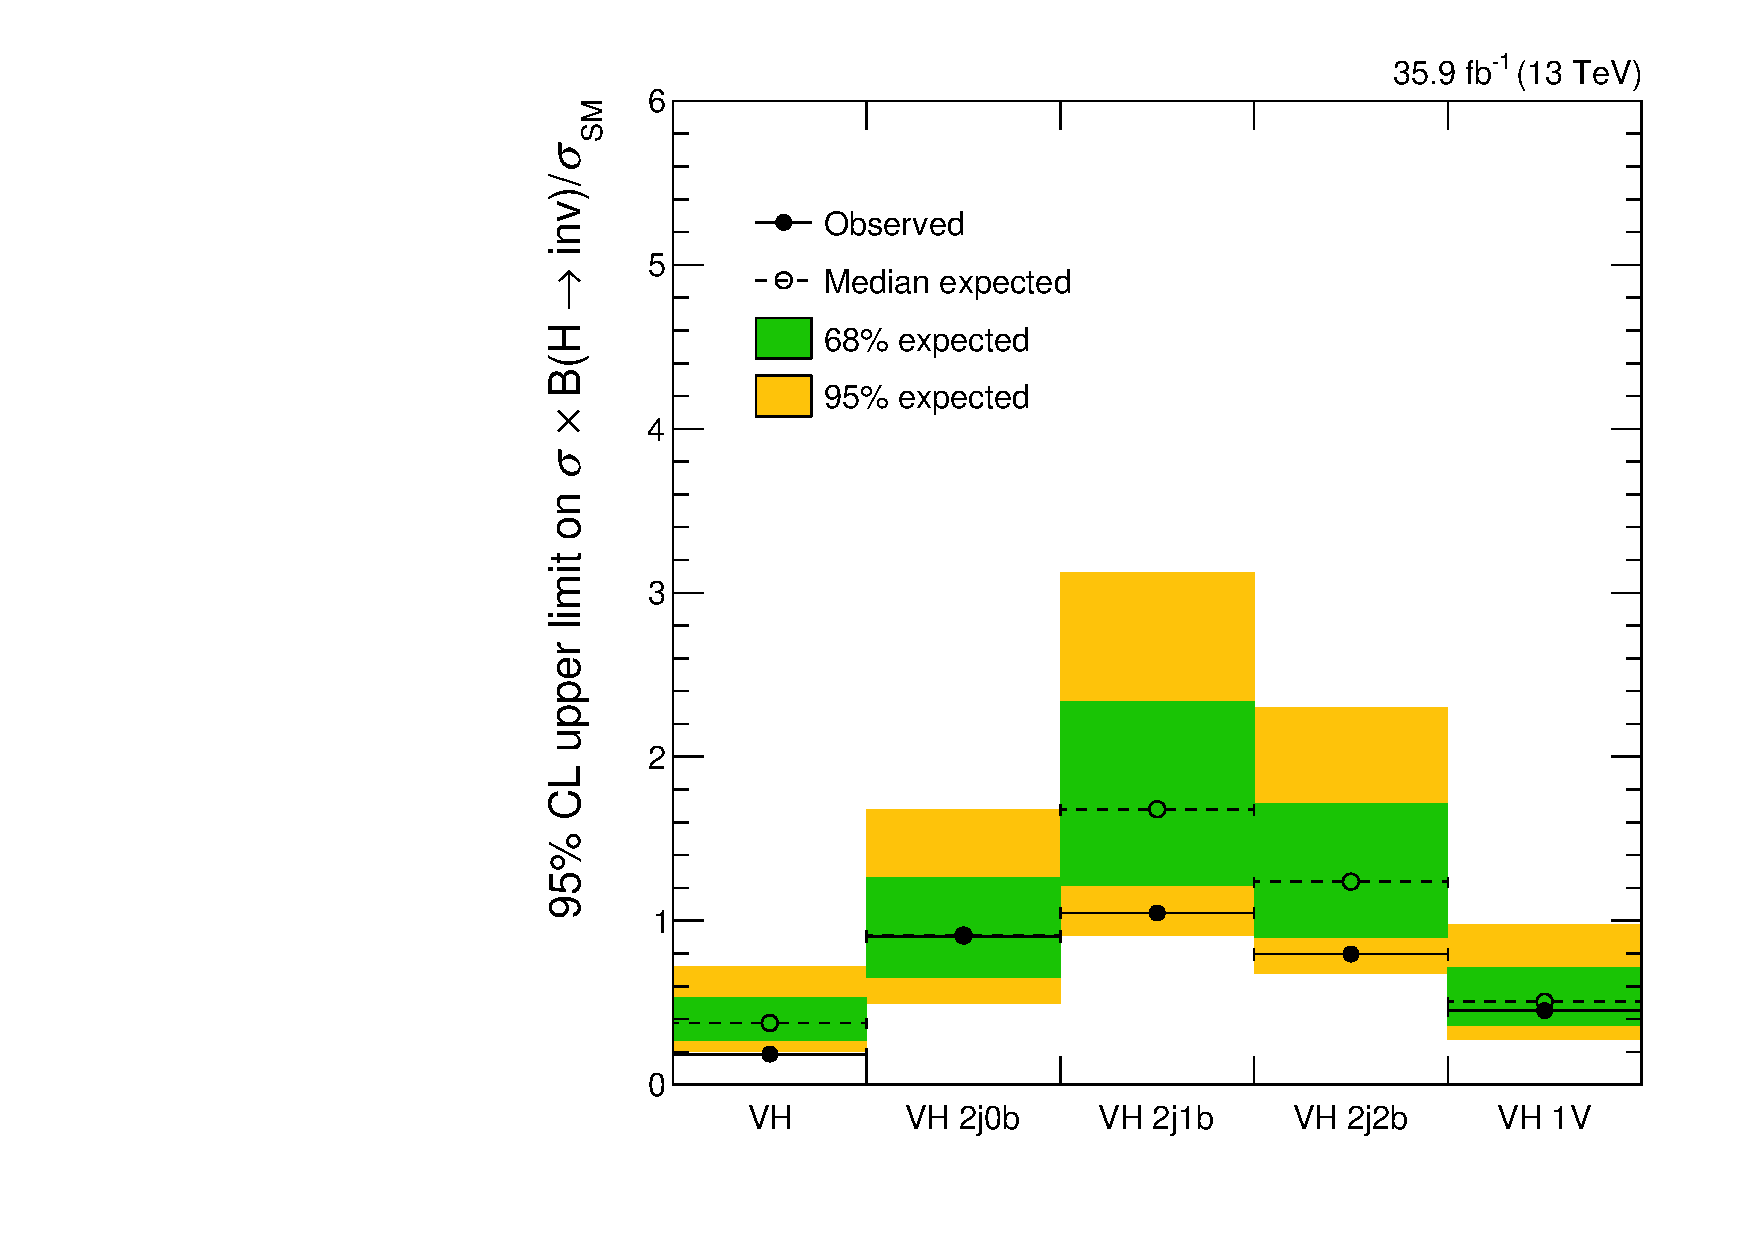
\includegraphics[width=\textwidth]{figures/limits/VH/limit_2016_VH.pdf}
        \caption{\VH --- 2016}
    \end{subfigure}
    \hfill
    \begin{subfigure}[b]{0.45\textwidth}
        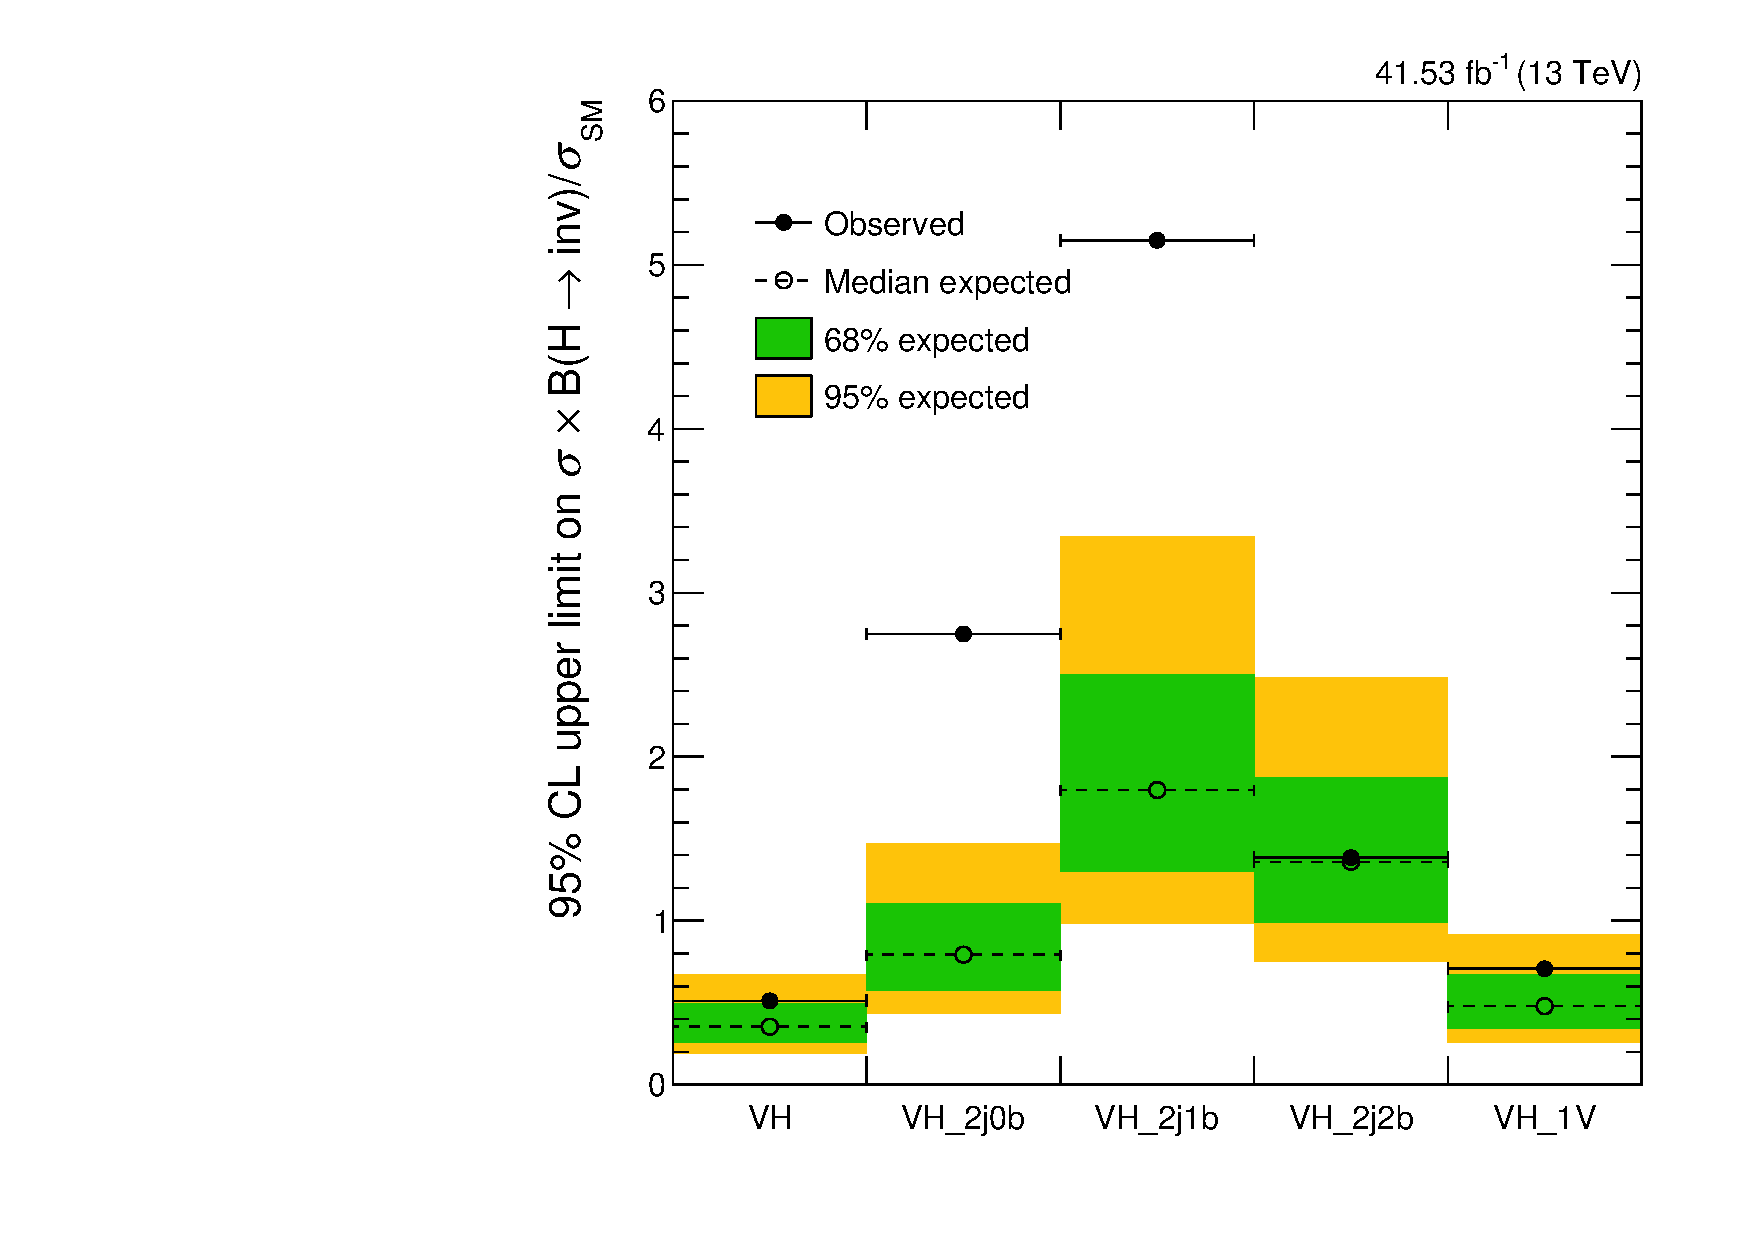
\includegraphics[width=\textwidth]{figures/limits/VH/limit_2017_VH.pdf}
        \caption{\VH --- 2017}
    \end{subfigure}

    \begin{subfigure}[b]{0.45\textwidth}
        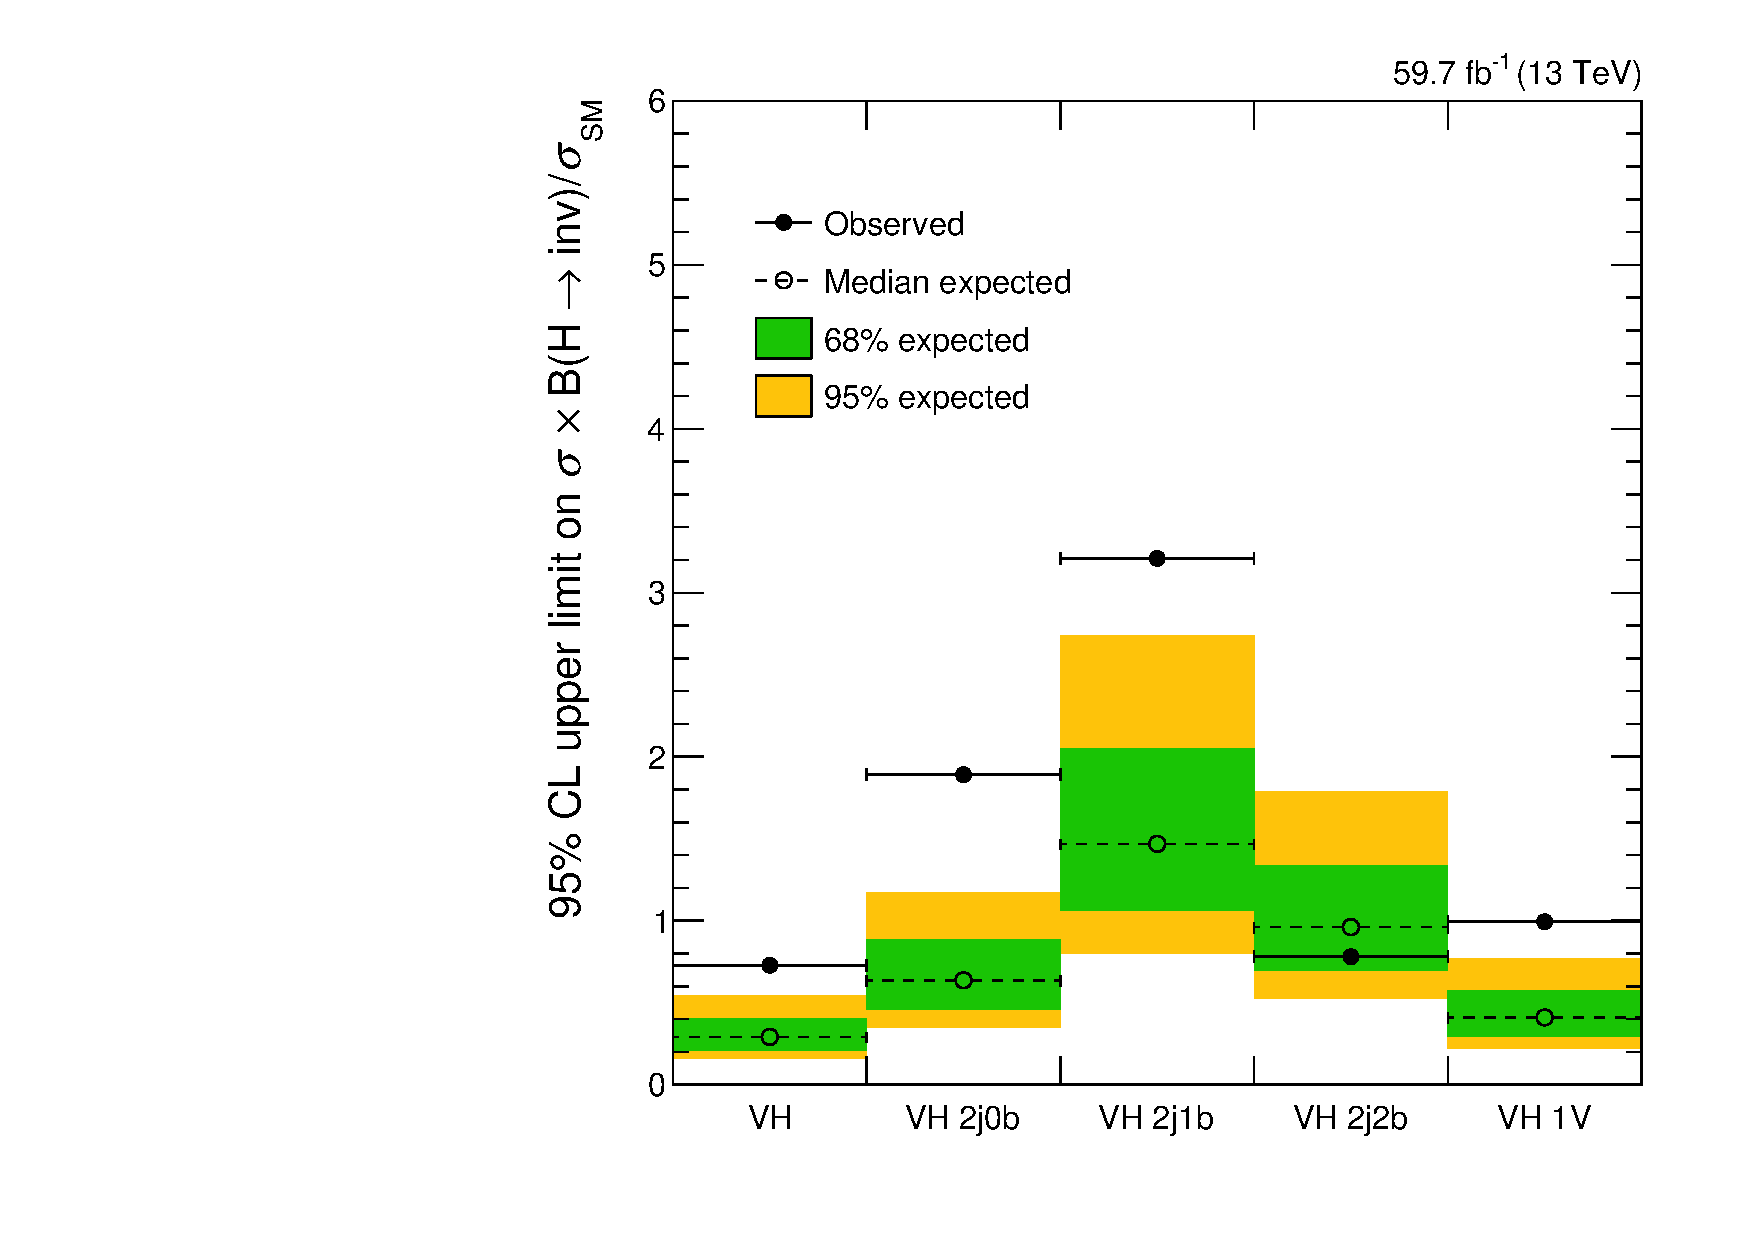
\includegraphics[width=\textwidth]{figures/limits/VH/limit_2018_VH.pdf}
        \caption{\VH --- 2018}
    \end{subfigure}
    \hfill
    \begin{subfigure}[b]{0.45\textwidth}
        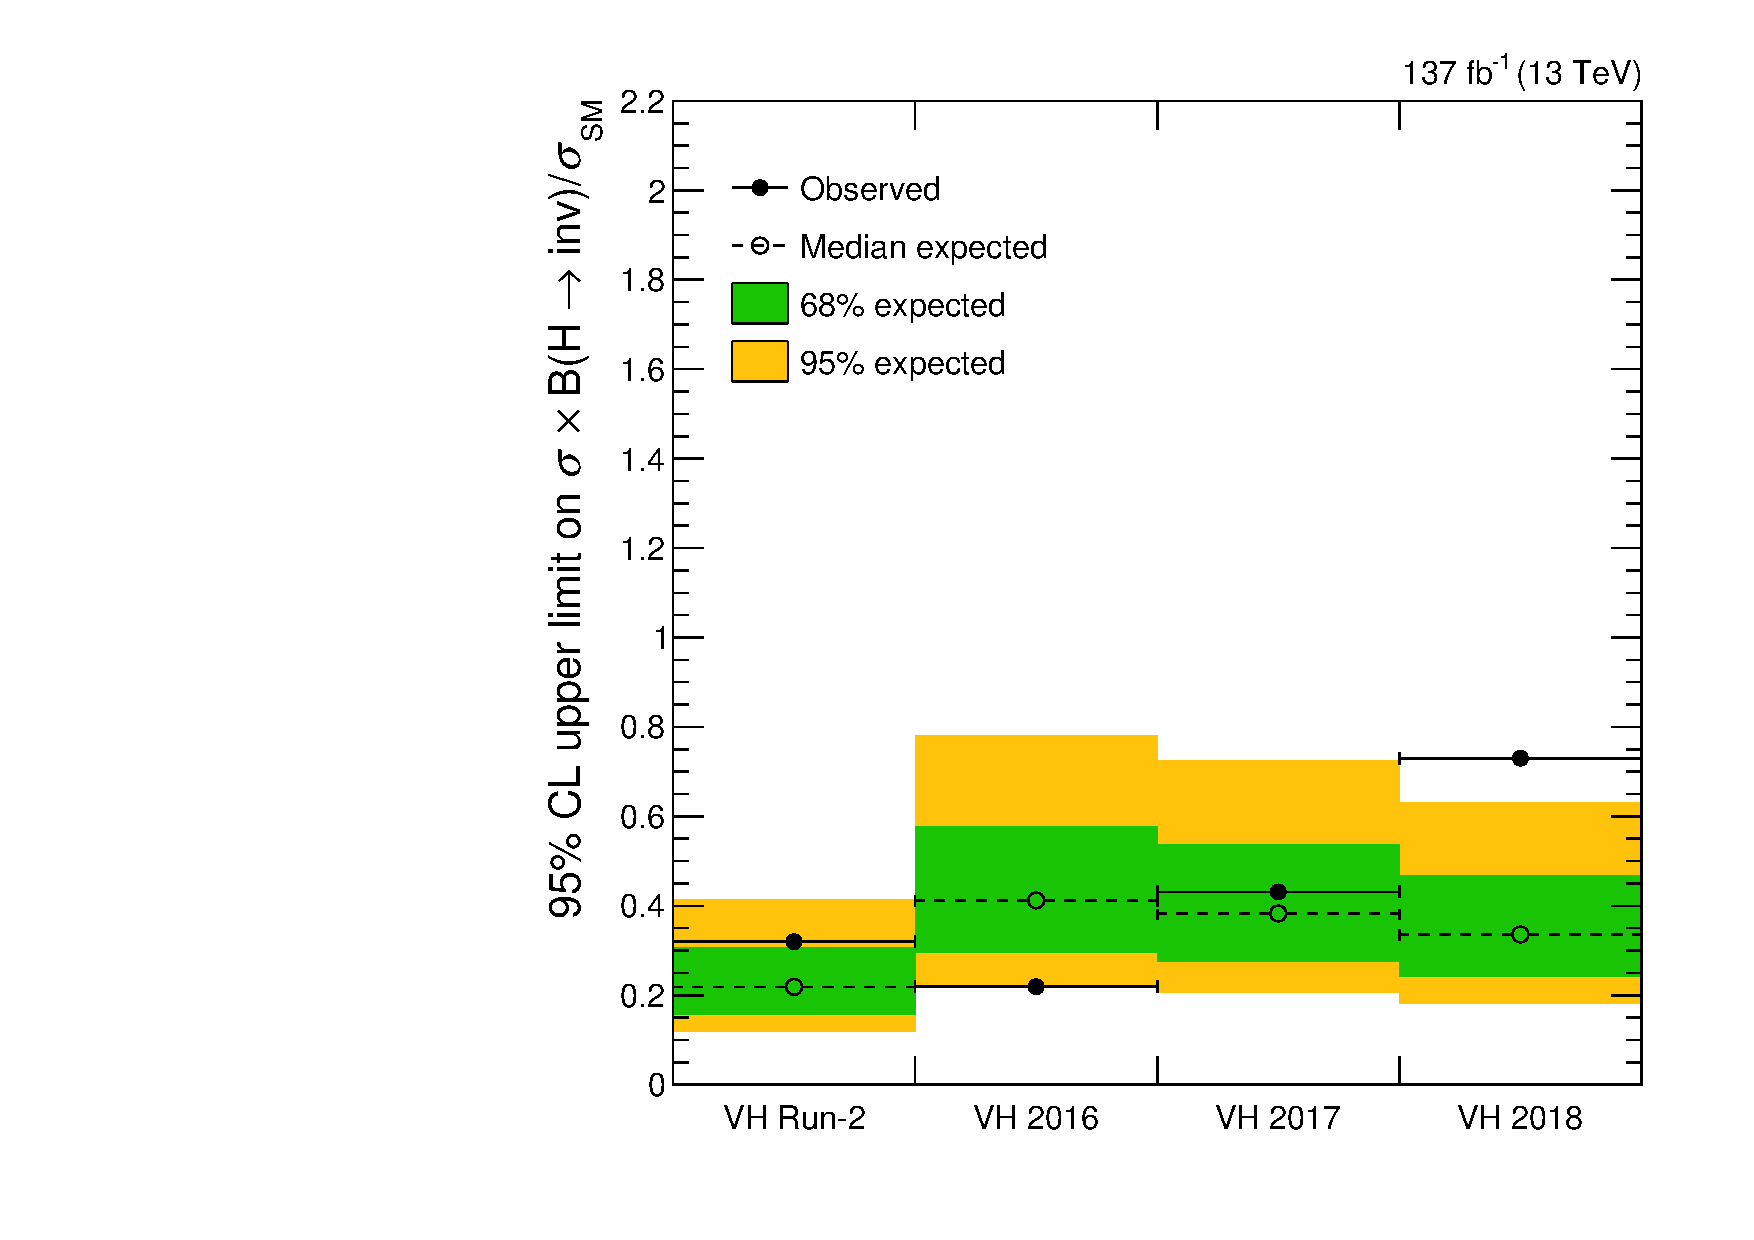
\includegraphics[width=\textwidth]{figures/limits/VH/limit_Run2_VH.pdf}
        \caption{\VH --- Run-2}
    \end{subfigure}
    \caption[Observed and expected 95\,\% CL upper limits on the Higgs boson to invisible state branching fraction in the \VH category, for both the individual subcategories, and the combination of them, for each data-taking year in Run-2]{Observed and expected 95\,\% CL upper limits on the Higgs boson to invisible state branching fraction in the \VH category, for both the individual subcategories, and the combination of them, for each data-taking year in Run-2.}
    \label{fig:htoinv_limit_VH}
\end{figure}

Distributions of the pre-fit and post-fit yields for 2016, 2017, and 2018 are displayed in Figs.~\ref{fig:htoinv_mountain_range_VH_2016}, \ref{fig:htoinv_mountain_range_VH_2017}, and \ref{fig:htoinv_mountain_range_VH_2018}, respectively.

\begin{figure}[htbp]
    \centering
    \begin{subfigure}[b]{0.9\textwidth}
        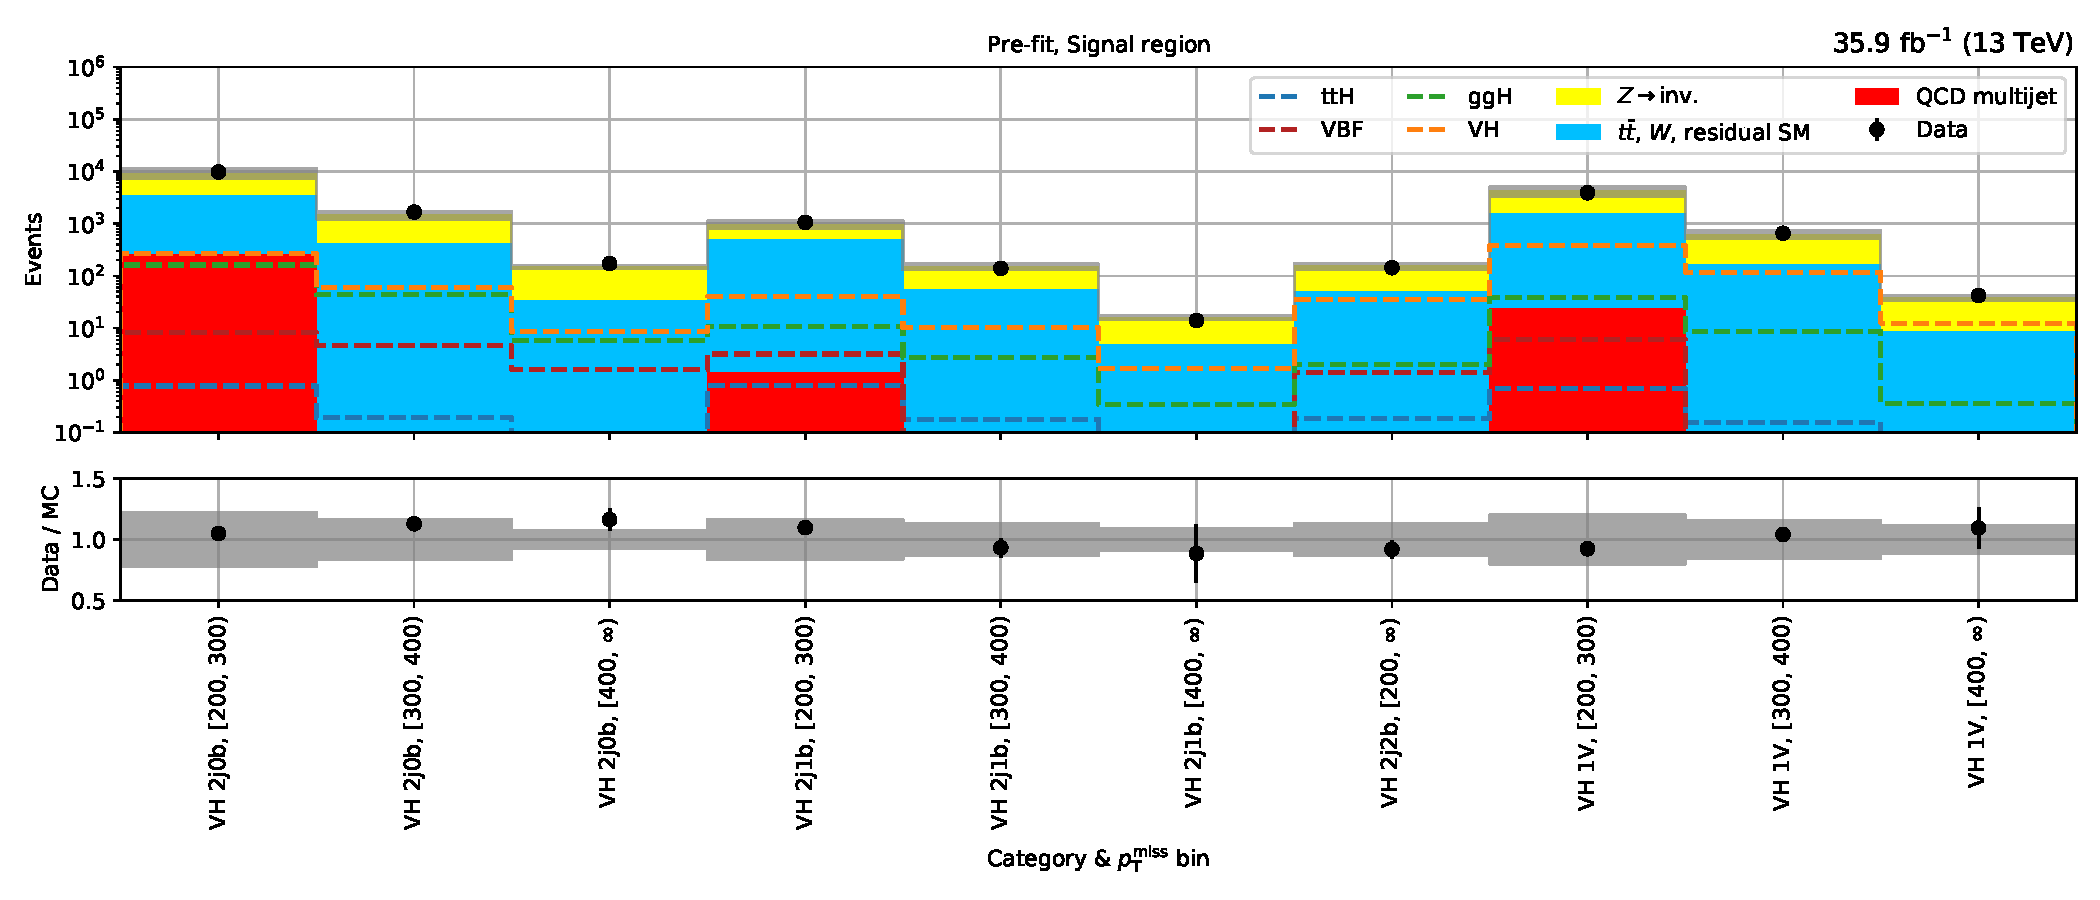
\includegraphics[width=\textwidth]{figures/mountain_ranges/2016/VH/SR_tree_prefit-abs_values_VH_cats.pdf}
        \caption{\VH --- 2016 (pre-fit)}
    \end{subfigure}

    \begin{subfigure}[b]{0.9\textwidth}
        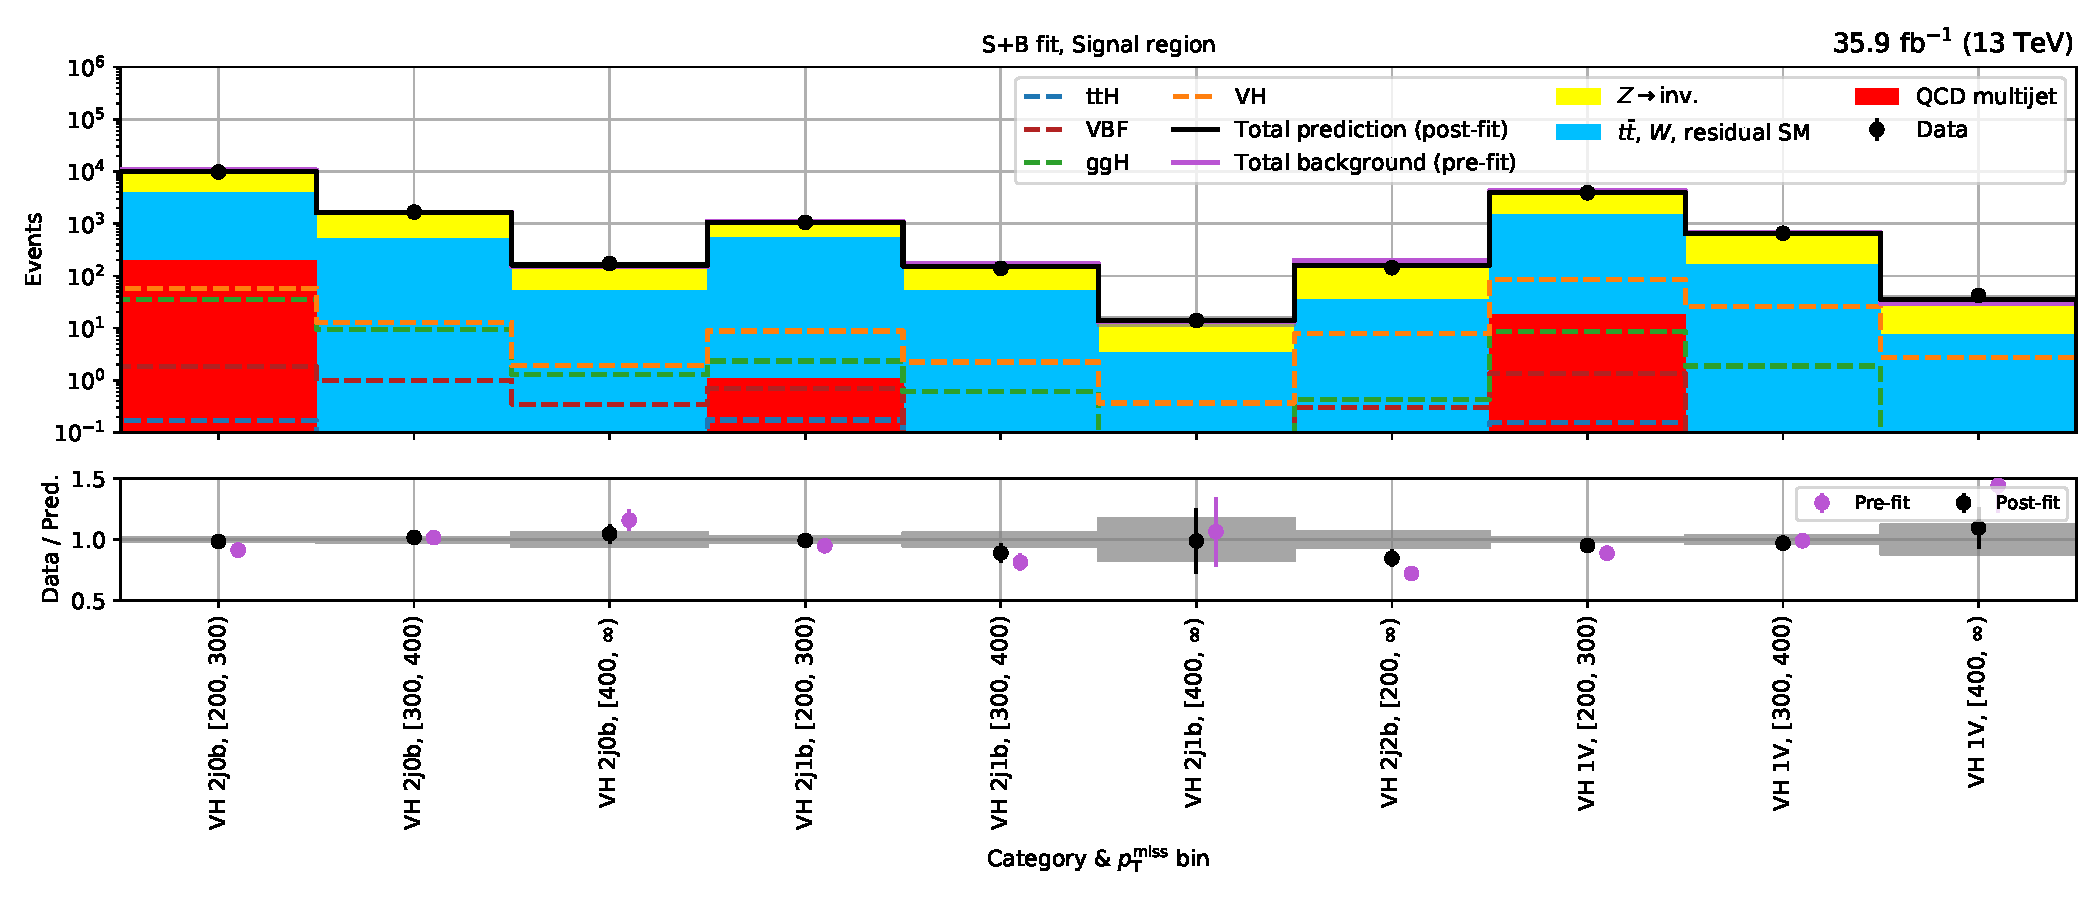
\includegraphics[width=\textwidth]{figures/mountain_ranges/2016/VH/SR_tree_fit_s-abs_values_VH_cats.pdf}
        \caption{\VH --- 2016 (post-fit)}
    \end{subfigure}
    \caption[Pre-fit and post-fit yields for each \VH subcategory and \ptmiss bin for the 2016 dataset]{Pre-fit and post-fit yields for each \VH subcategory and \ptmiss bin for the 2016 dataset. In bottom panel of post-fit plot, the ratio data to signal plus background is calculated.}
    \label{fig:htoinv_mountain_range_VH_2016}
\end{figure}

\begin{figure}[htbp]
    \centering
    \begin{subfigure}[b]{0.9\textwidth}
        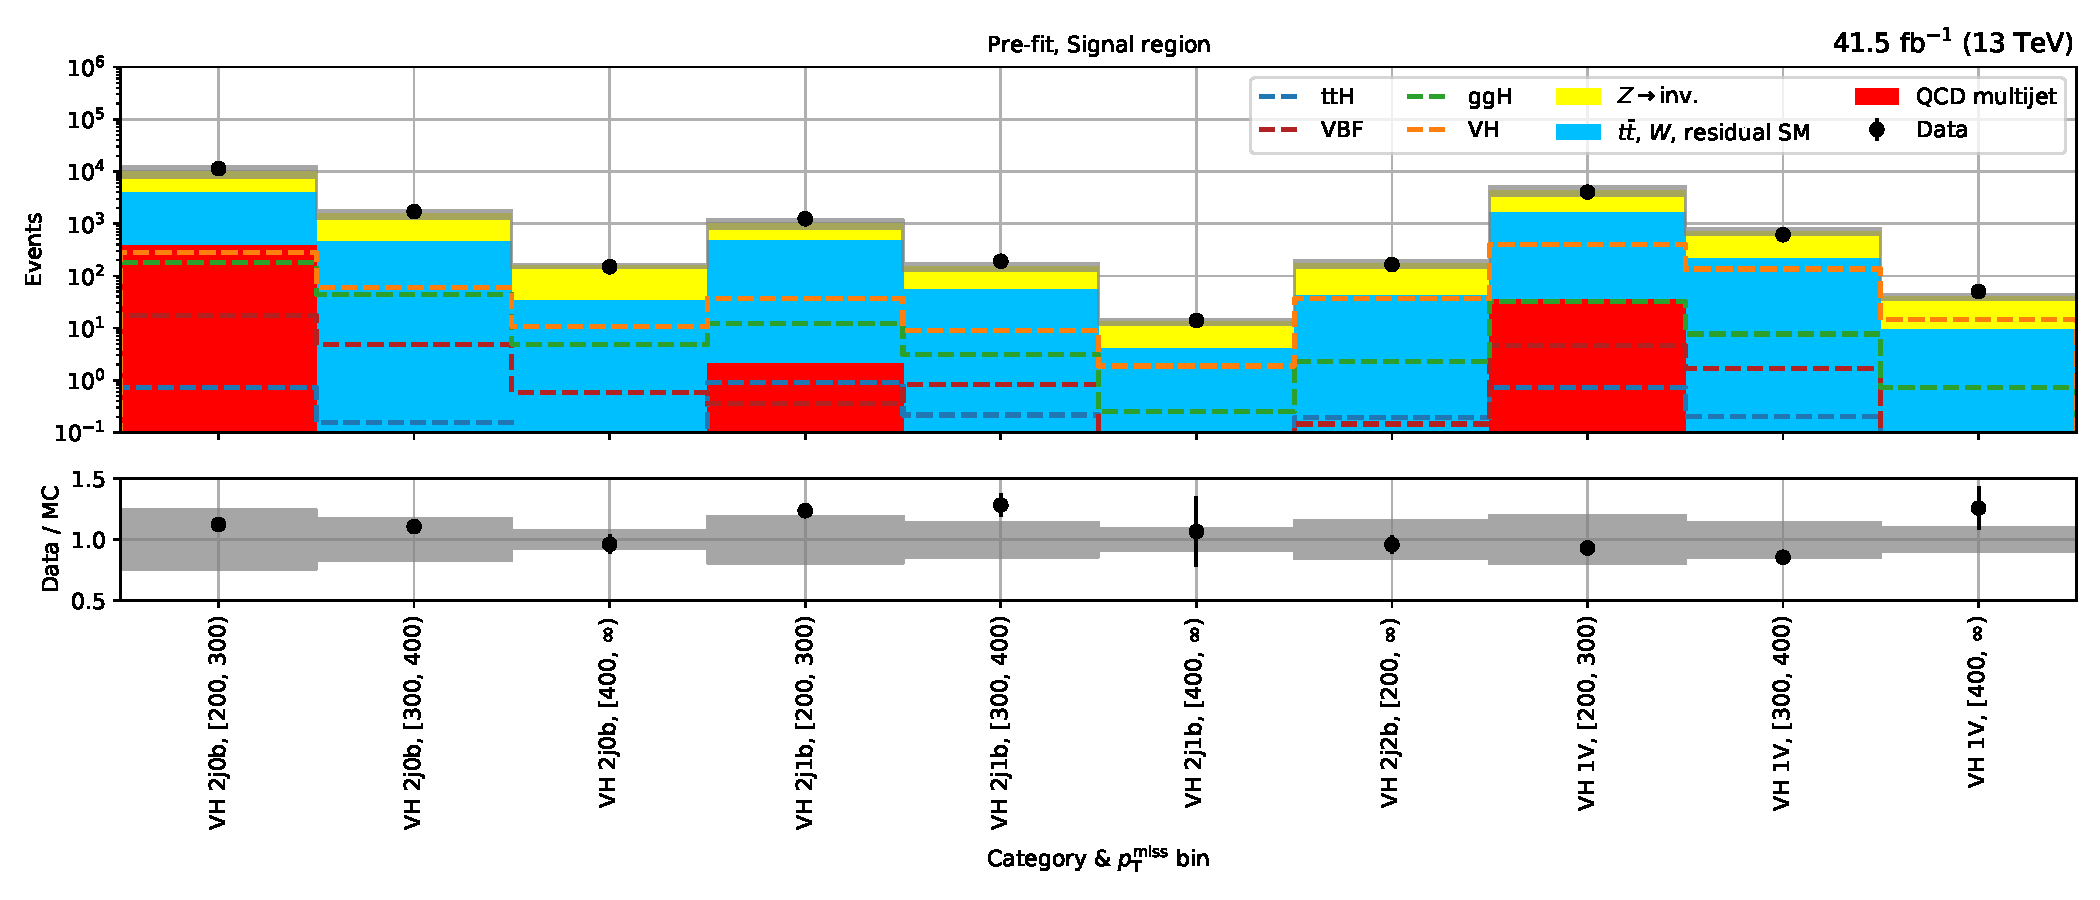
\includegraphics[width=\textwidth]{figures/mountain_ranges/2017/VH/SR_tree_prefit-abs_values_VH_cats.pdf}
        \caption{\VH --- 2017 (pre-fit)}
    \end{subfigure}

    \begin{subfigure}[b]{0.9\textwidth}
        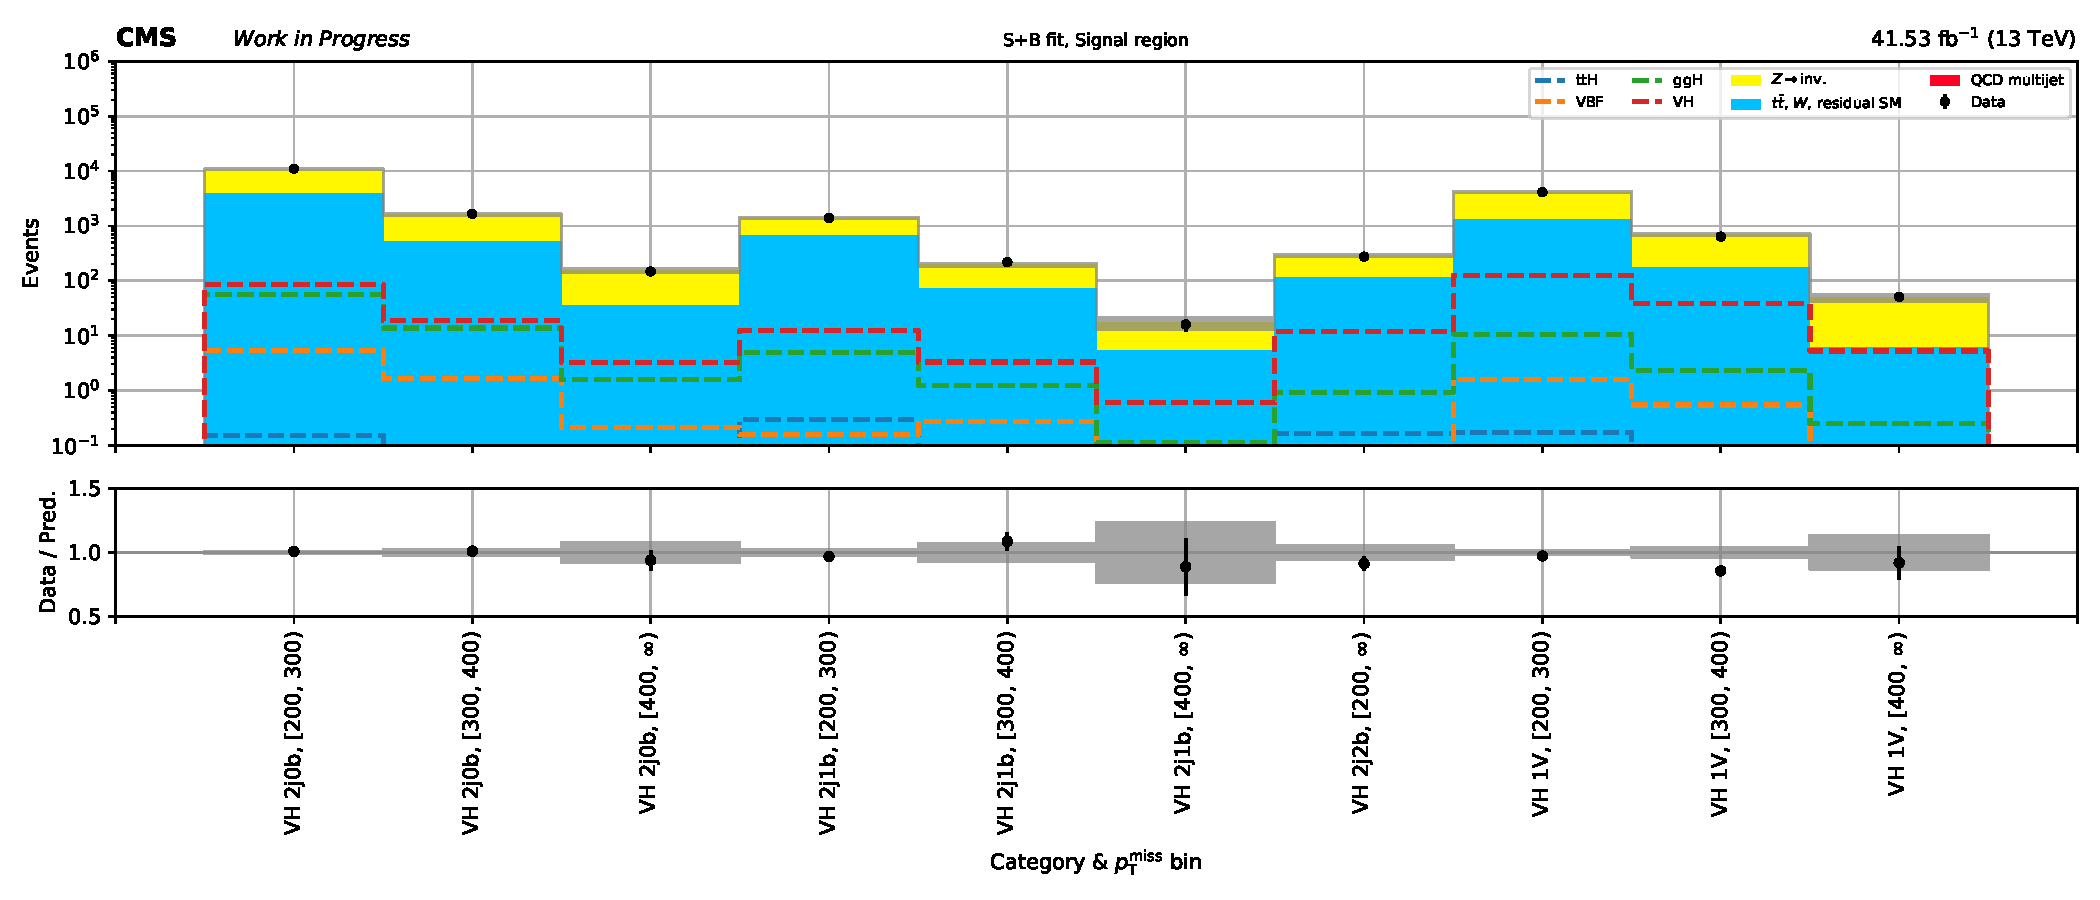
\includegraphics[width=\textwidth]{figures/mountain_ranges/2017/VH/SR_tree_fit_s-abs_values_VH_cats.pdf}
        \caption{\VH --- 2017 (post-fit)}
    \end{subfigure}
    \caption[Pre-fit and post-fit yields for each \VH subcategory and \ptmiss bin for the 2017 dataset]{Pre-fit and post-fit yields for each \VH subcategory and \ptmiss bin for the 2017 dataset. In bottom panel of post-fit plot, the ratio data to signal plus background is calculated.}
    \label{fig:htoinv_mountain_range_VH_2017}
\end{figure}

\begin{figure}[htbp]
    \centering
    \begin{subfigure}[b]{0.9\textwidth}
        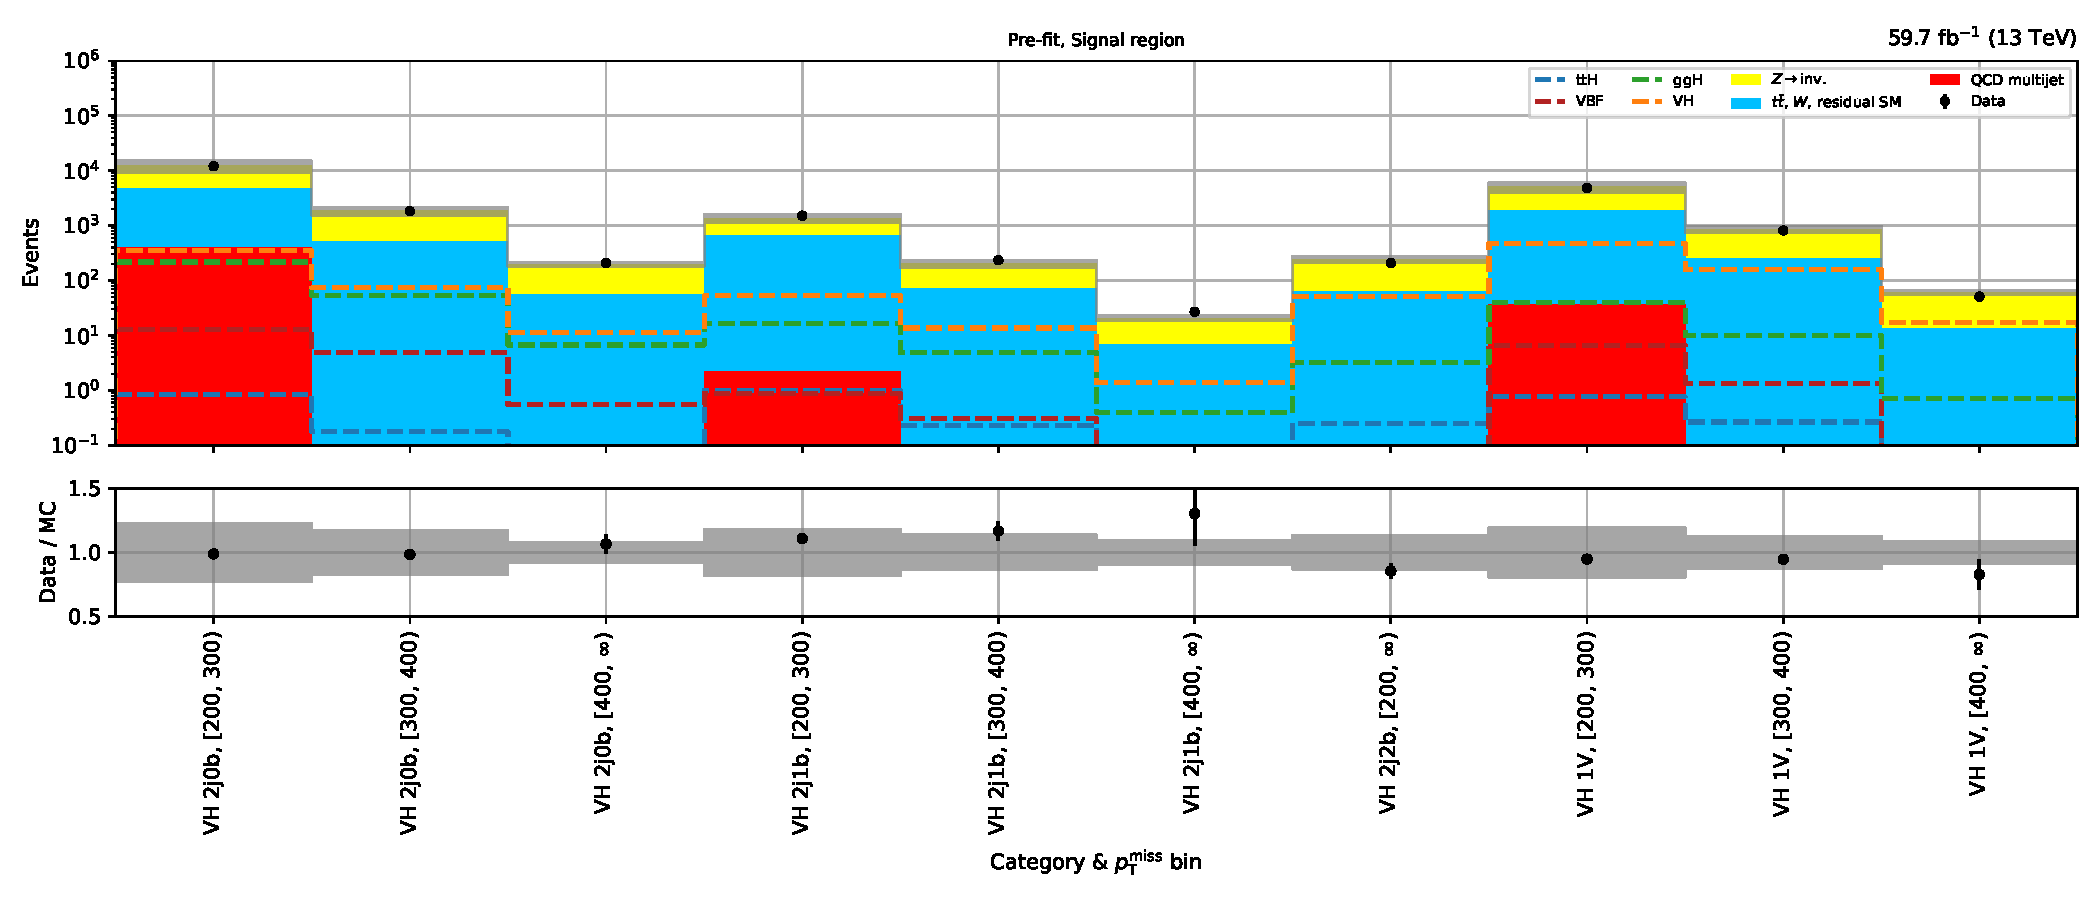
\includegraphics[width=\textwidth]{figures/mountain_ranges/2018/VH/SR_tree_prefit-abs_values_VH_cats.pdf}
        \caption{\VH --- 2018 (pre-fit)}
    \end{subfigure}

    \begin{subfigure}[b]{0.9\textwidth}
        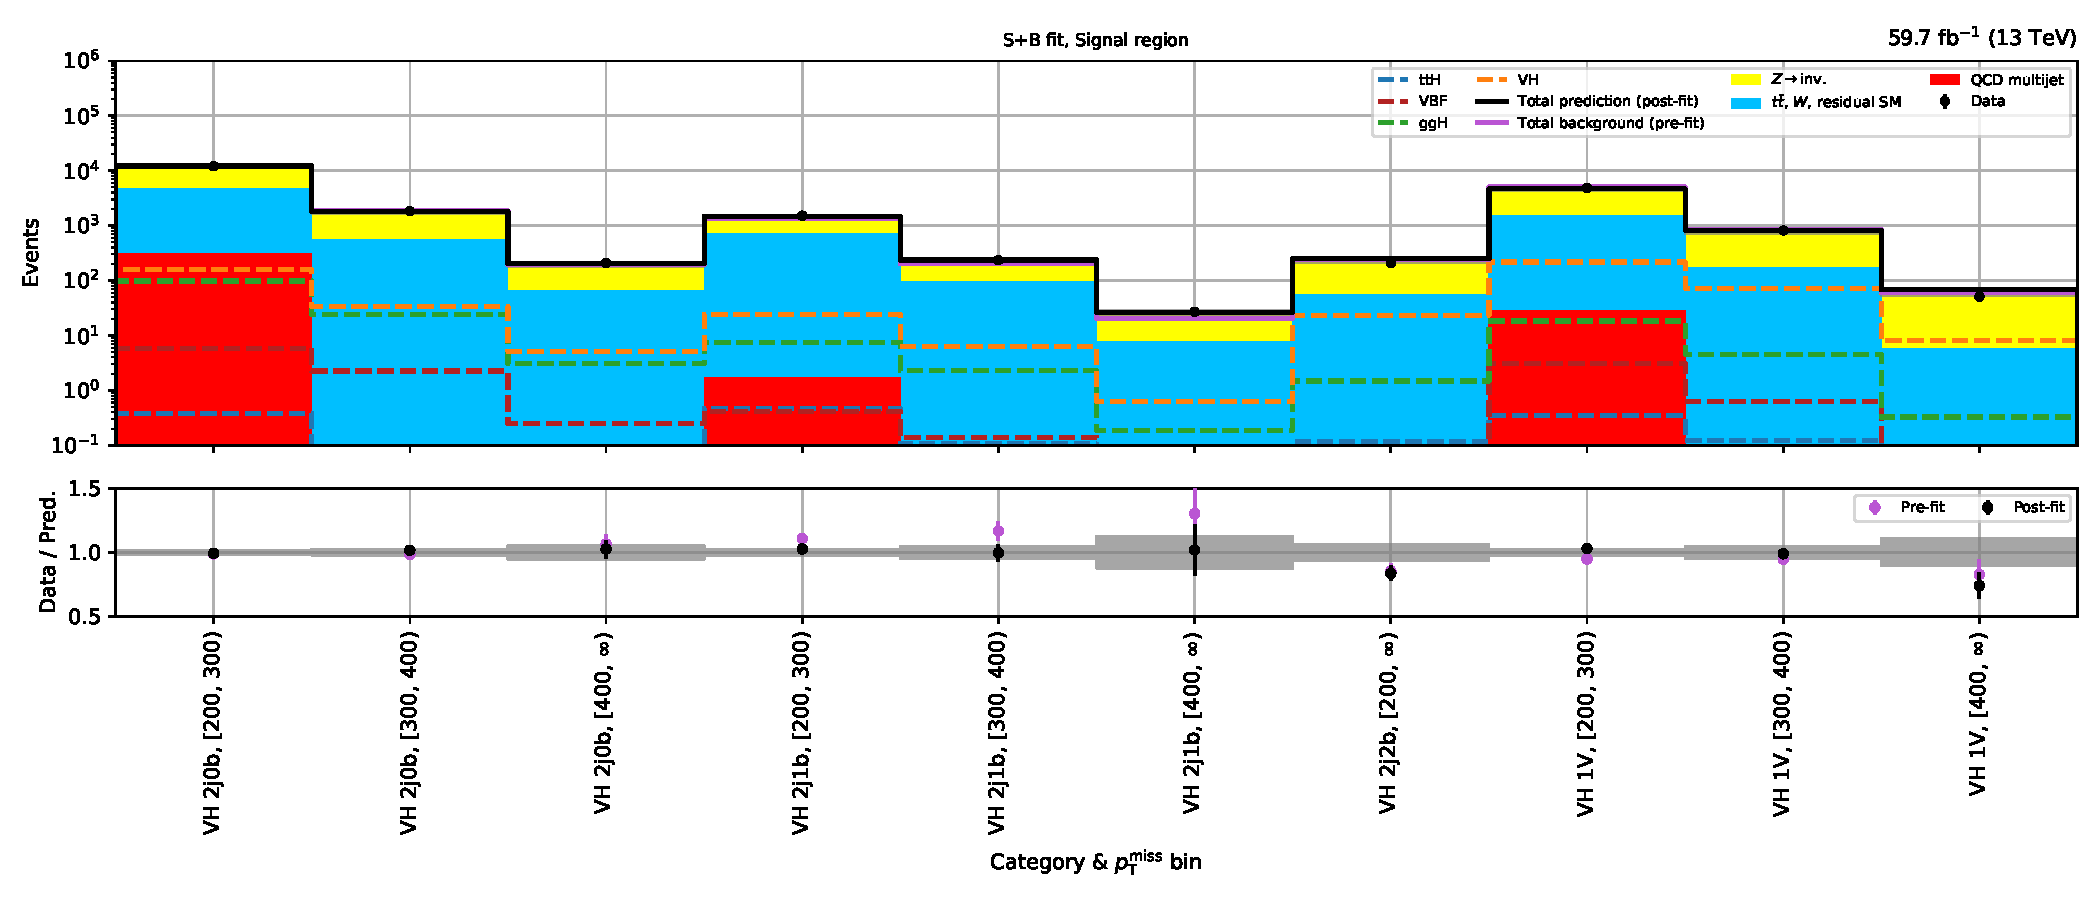
\includegraphics[width=\textwidth]{figures/mountain_ranges/2018/VH/SR_tree_fit_s-abs_values_VH_cats.pdf}
        \caption{\VH --- 2018 (post-fit)}
    \end{subfigure}
    \caption[Pre-fit and post-fit yields for each \VH subcategory and \ptmiss bin for the 2018 dataset]{Pre-fit and post-fit yields for each \VH subcategory and \ptmiss bin for the 2018 dataset. In bottom panel of post-fit plot, the ratio data to signal plus background is calculated.}
    \label{fig:htoinv_mountain_range_VH_2018}
\end{figure}

\clearpage


%=========================================================


\section{Analysis of the \texorpdfstring{\ggH}{ggH} mode}
\label{sec:htoinv_analysis_ggF}

As with the \VH category, all of the \glspl{CR} are involved in estimating the non-multijet backgrounds in the signal region of the \ggH category. Equivalently to \ttH, the \acrshort{qcd} presence is derived using the tight and loose double sidebands. The category fractions \catFraction are calculated by the former, while the remaining terms in Eq.~\ref{eq:qcd_prediction} are computed from the latter.

Expected and observed limits on the signal strength parameter are presented in Fig.~\ref{fig:htoinv_limit_ggF} for each \ggH subcategory and their combination in each data taking year as well as over the full Run-2 dataset.

\begin{figure}[htbp]
    \centering
    \begin{subfigure}[b]{0.45\textwidth}
        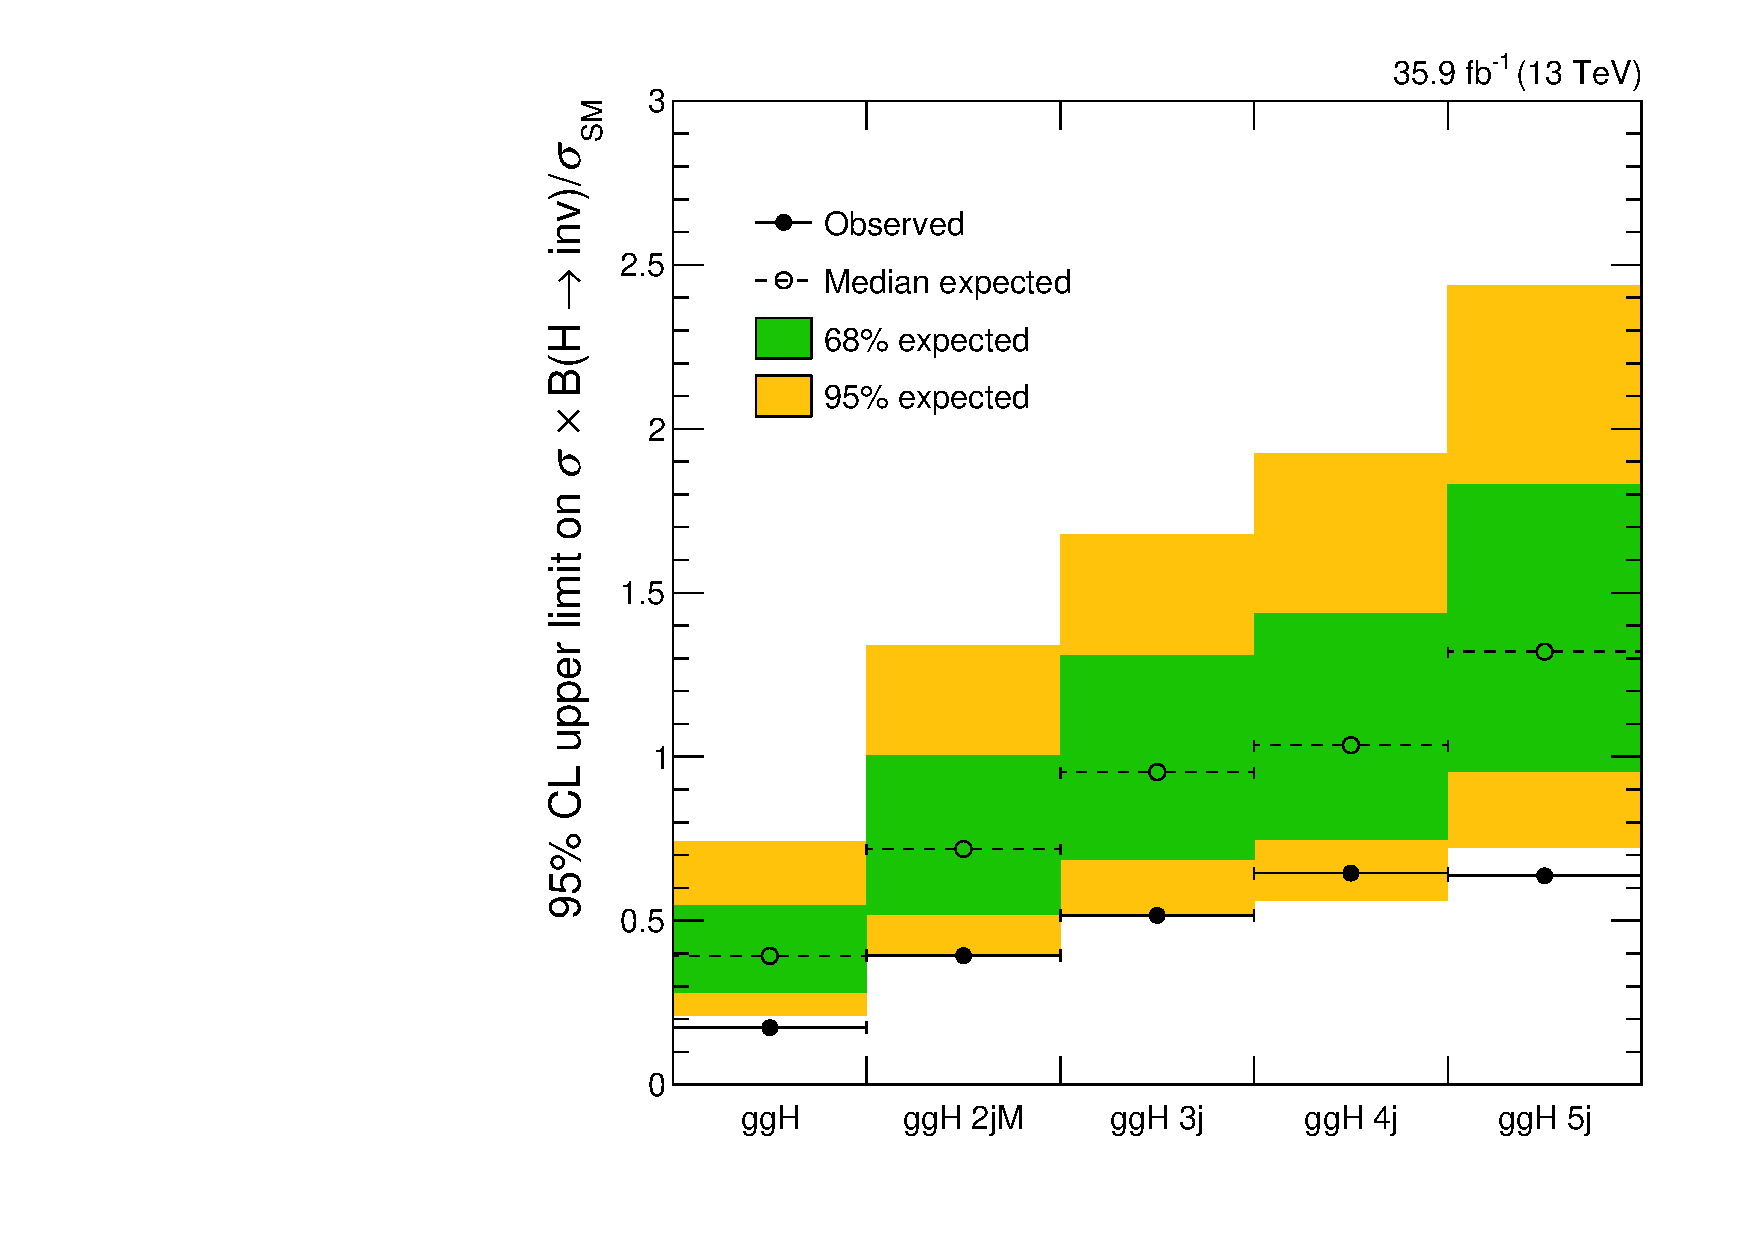
\includegraphics[width=\textwidth]{figures/limits/ggF/limit_2016_ggF.pdf}
        \caption{\ggH --- 2016}
    \end{subfigure}
    \hfill
    \begin{subfigure}[b]{0.45\textwidth}
        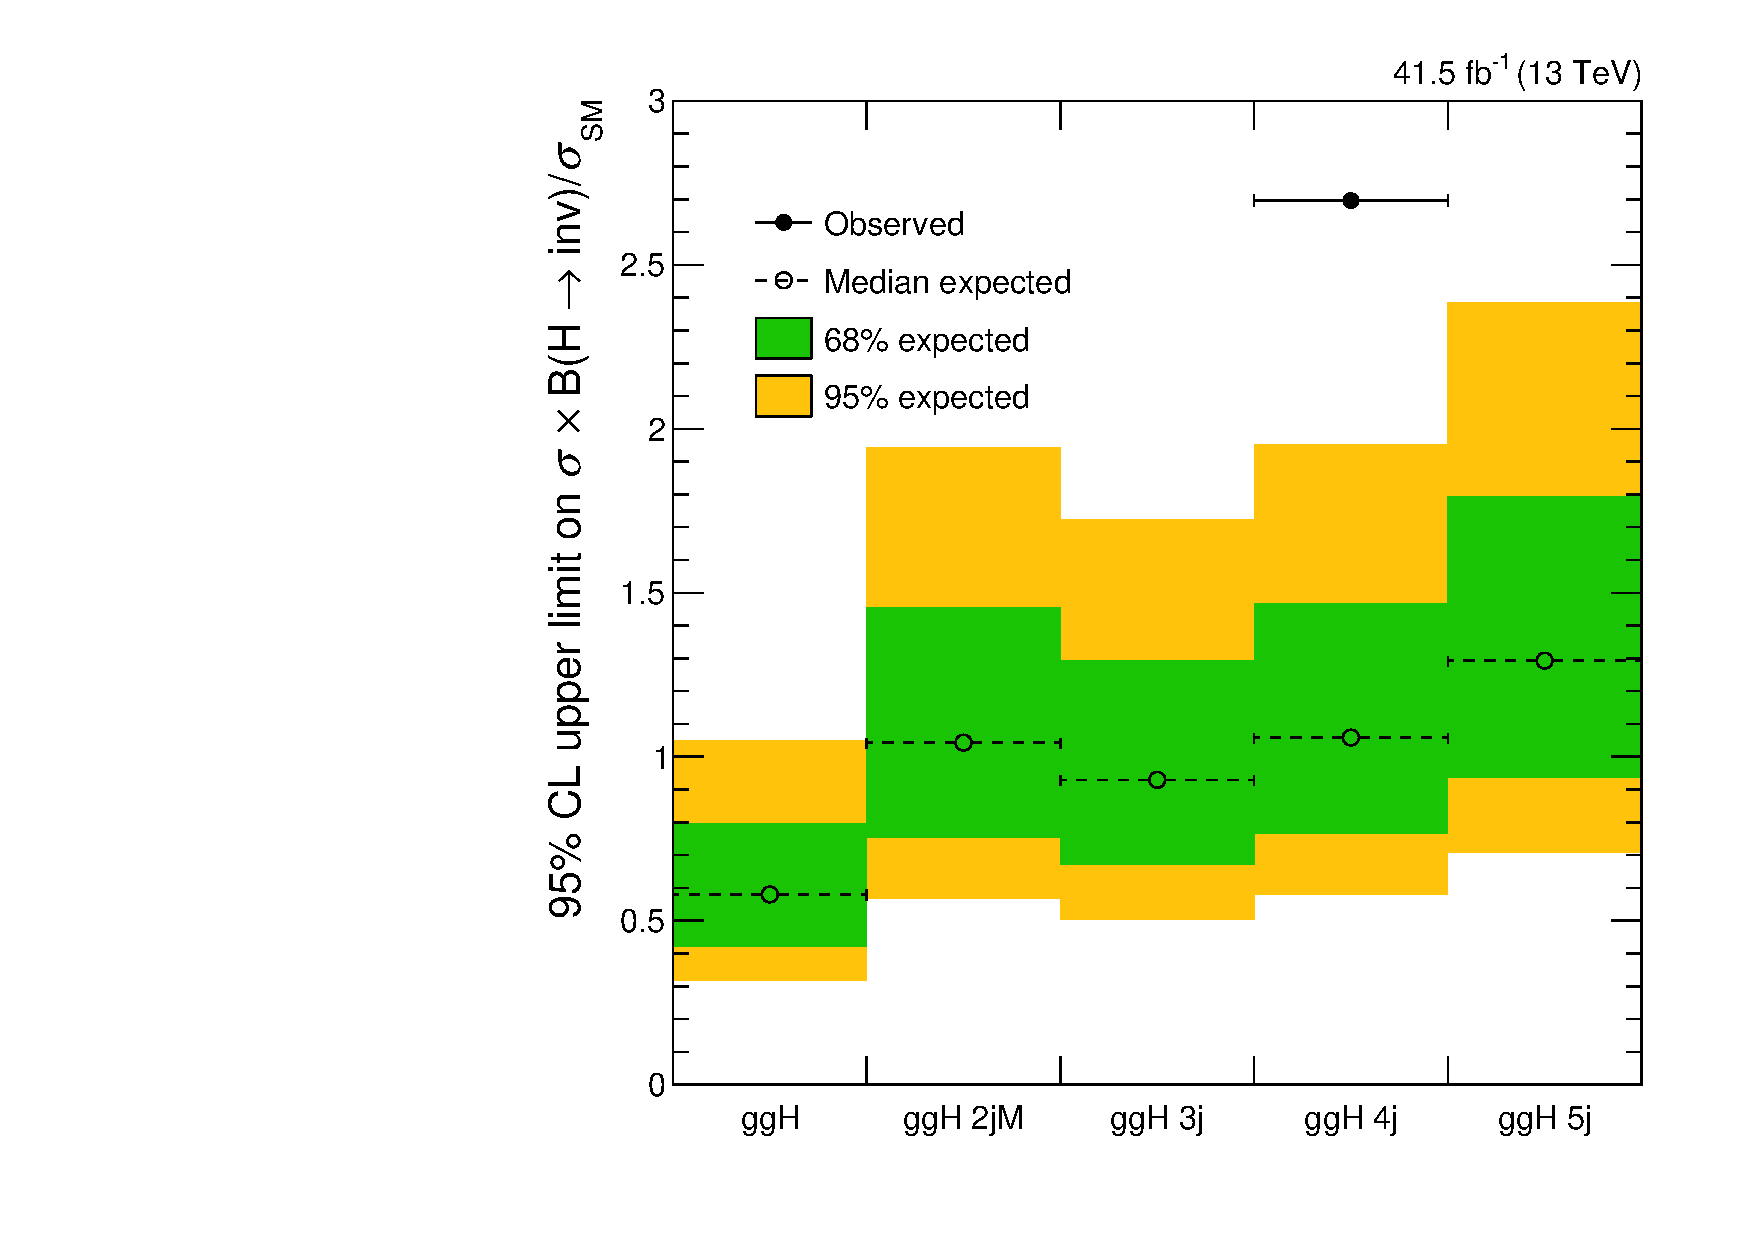
\includegraphics[width=\textwidth]{figures/limits/ggF/limit_2017_ggF.pdf}
        \caption{\ggH --- 2017}
    \end{subfigure}

    \begin{subfigure}[b]{0.45\textwidth}
        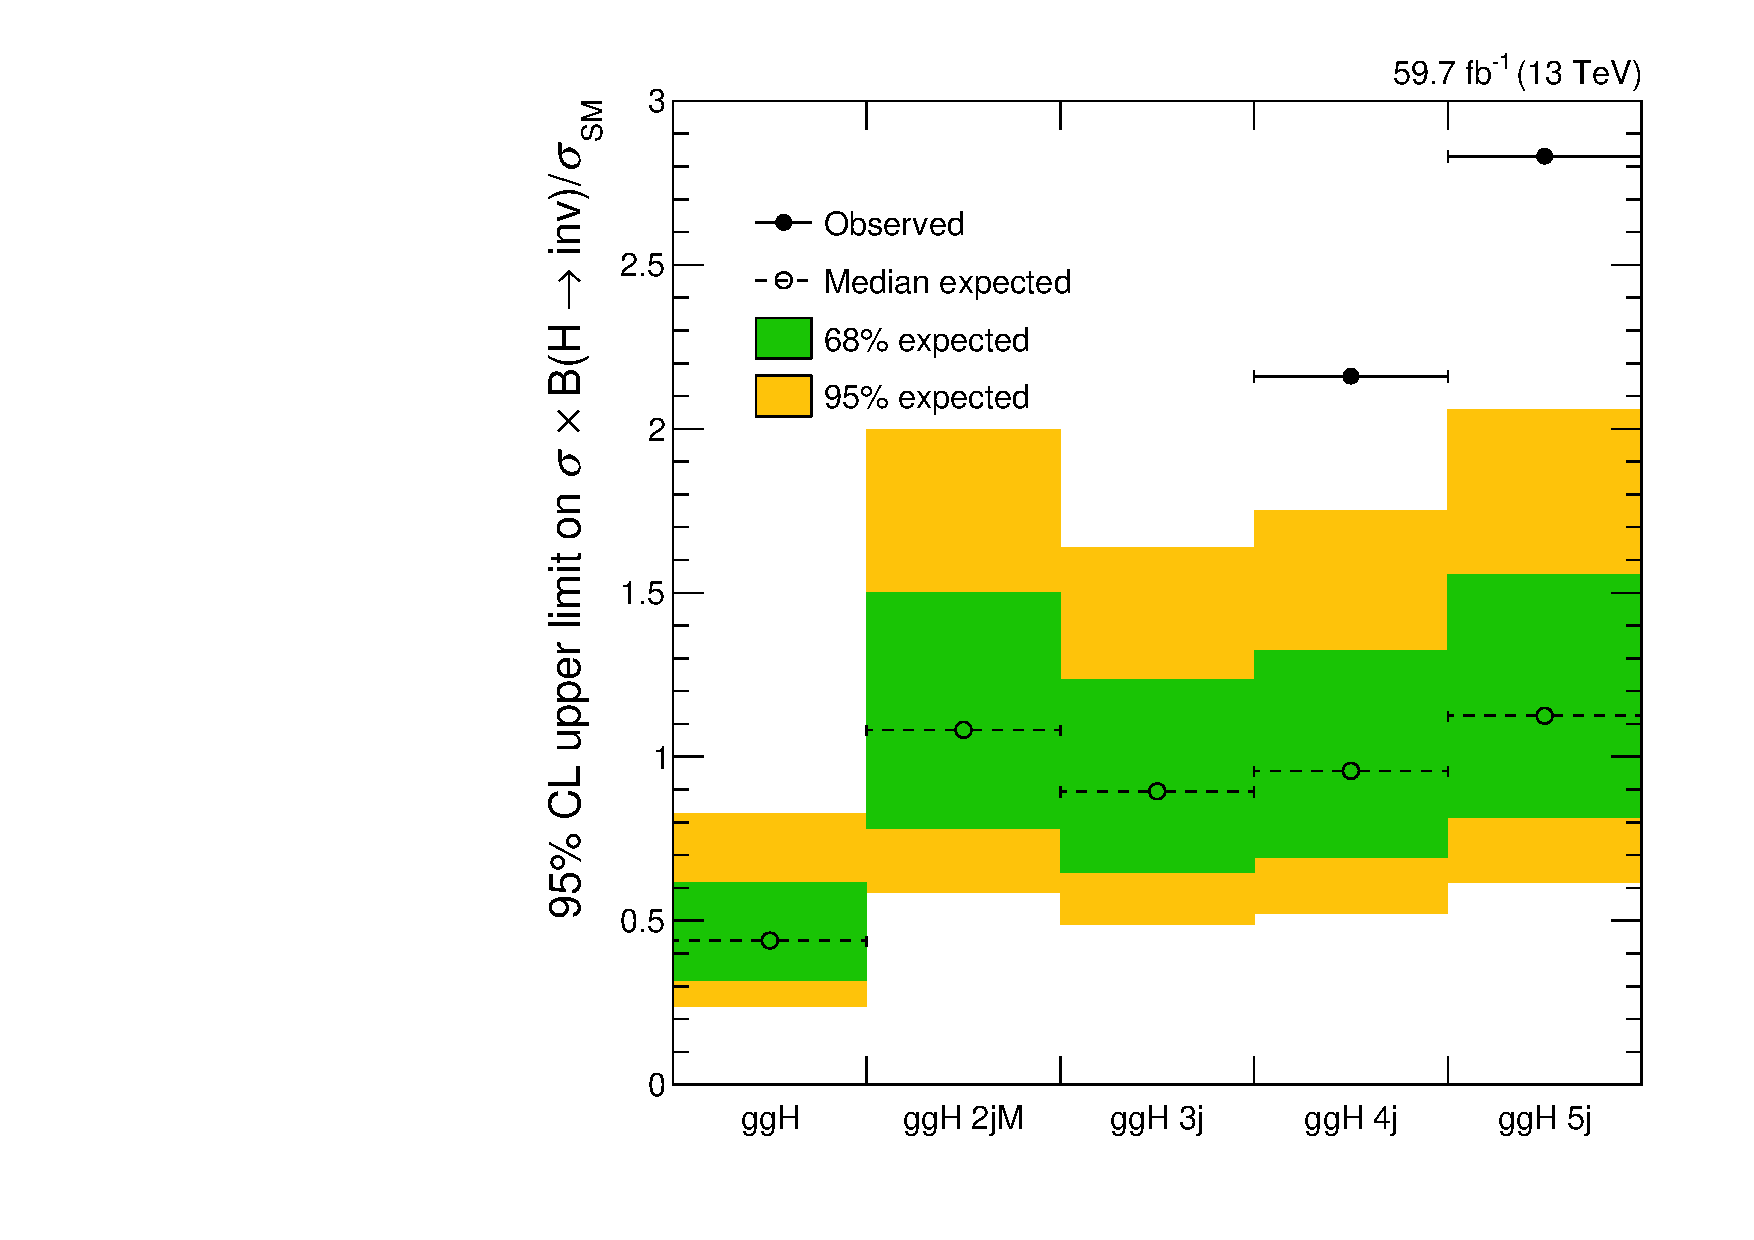
\includegraphics[width=\textwidth]{figures/limits/ggF/limit_2018_ggF.pdf}
        \caption{\ggH --- 2018}
    \end{subfigure}
    \hfill
    \begin{subfigure}[b]{0.45\textwidth}
        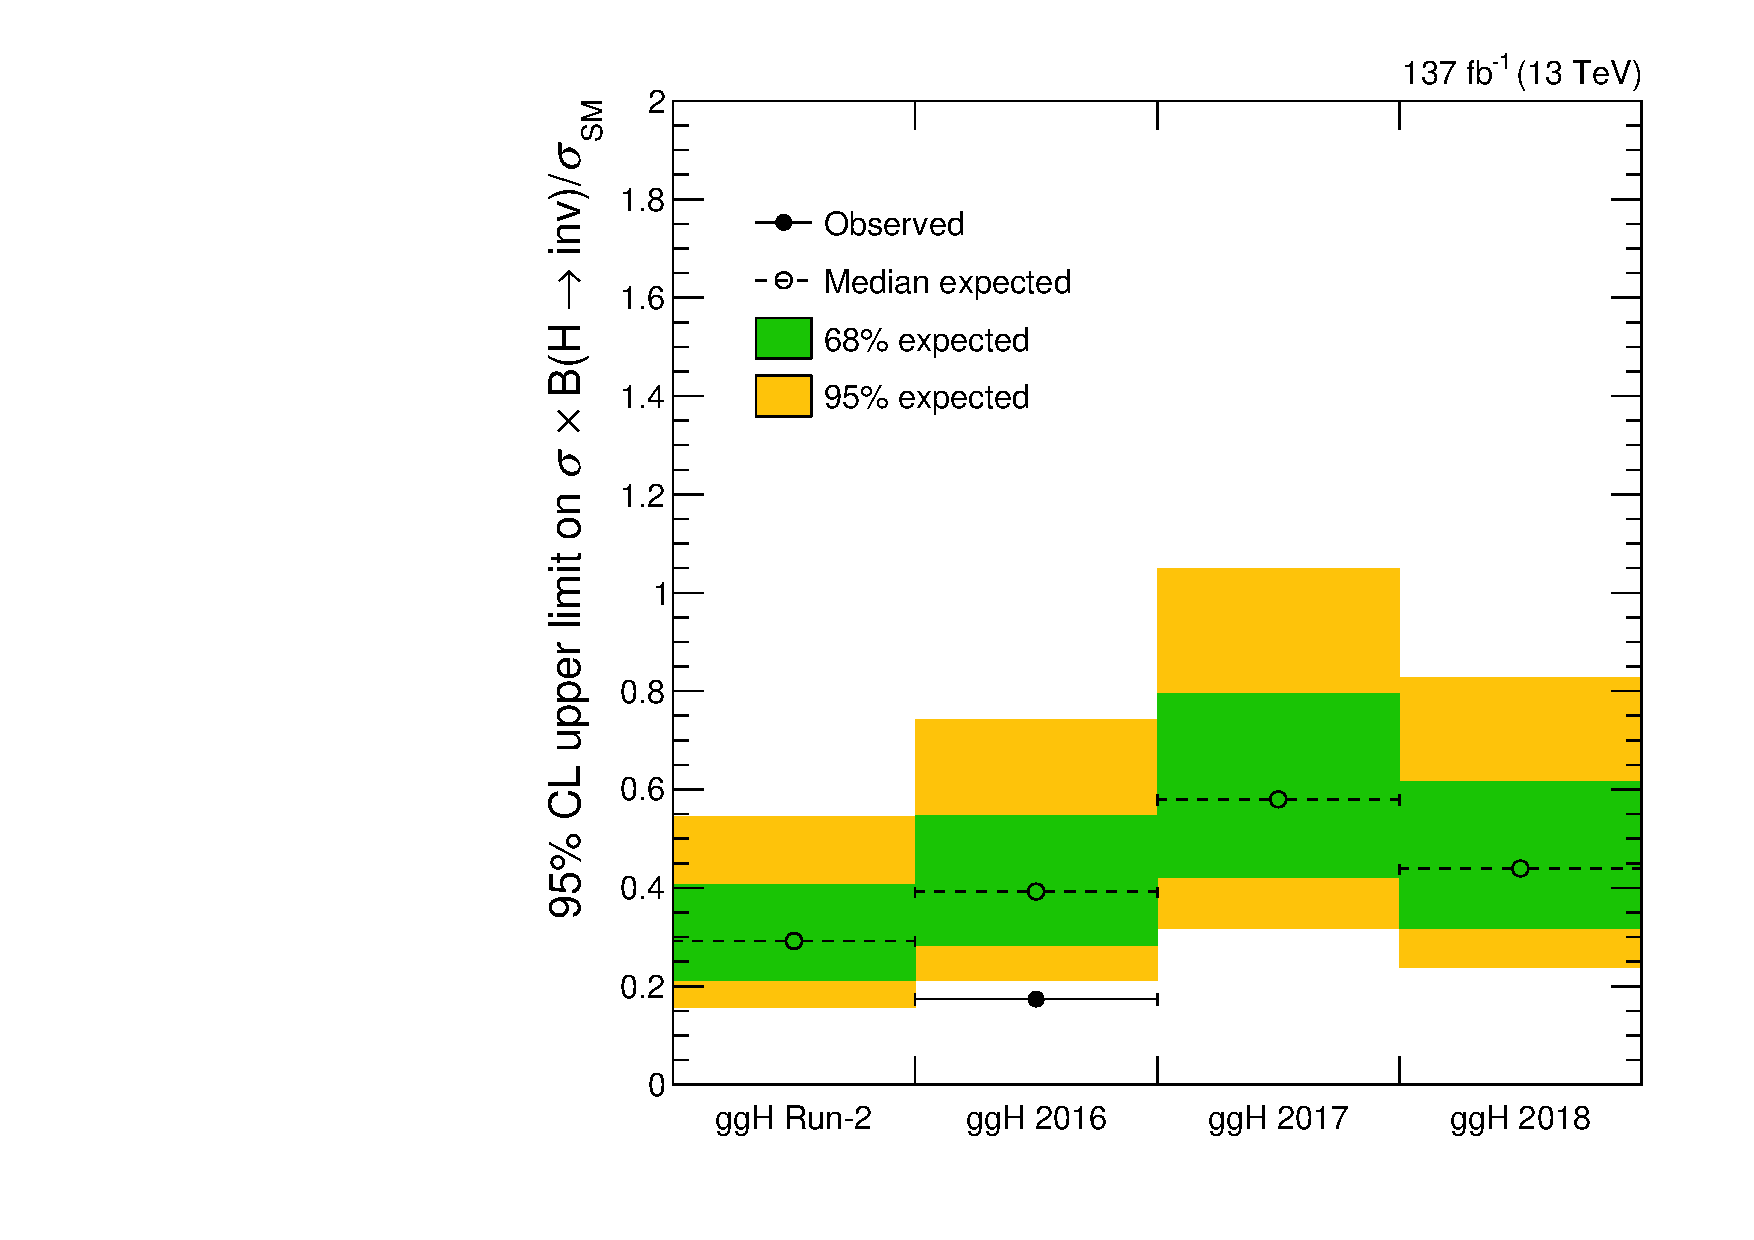
\includegraphics[width=\textwidth]{figures/limits/ggF/limit_Run2_ggF.pdf}
        \caption{\ggH --- Run-2}
    \end{subfigure}
    \caption[Observed and expected 95\,\% CL upper limits on the Higgs boson to invisible state branching fraction in the \ggH category, for both the individual subcategories, and the combination of them, for each data-taking year in Run-2]{Observed and expected 95\,\% CL upper limits on the Higgs boson to invisible state branching fraction in the \ggH category, for both the individual subcategories, and the combination of them, for each data-taking year in Run-2.}
    \label{fig:htoinv_limit_ggF}
\end{figure}

Distributions of the pre-fit and post-fit yields for 2016, 2017, and 2018 are displayed in Figs.~\ref{fig:htoinv_mountain_range_ggH_2016}, \ref{fig:htoinv_mountain_range_ggH_2017}, and \ref{fig:htoinv_mountain_range_ggH_2018}, respectively.

\begin{figure}[htbp]
    \centering
    \begin{subfigure}[b]{0.9\textwidth}
        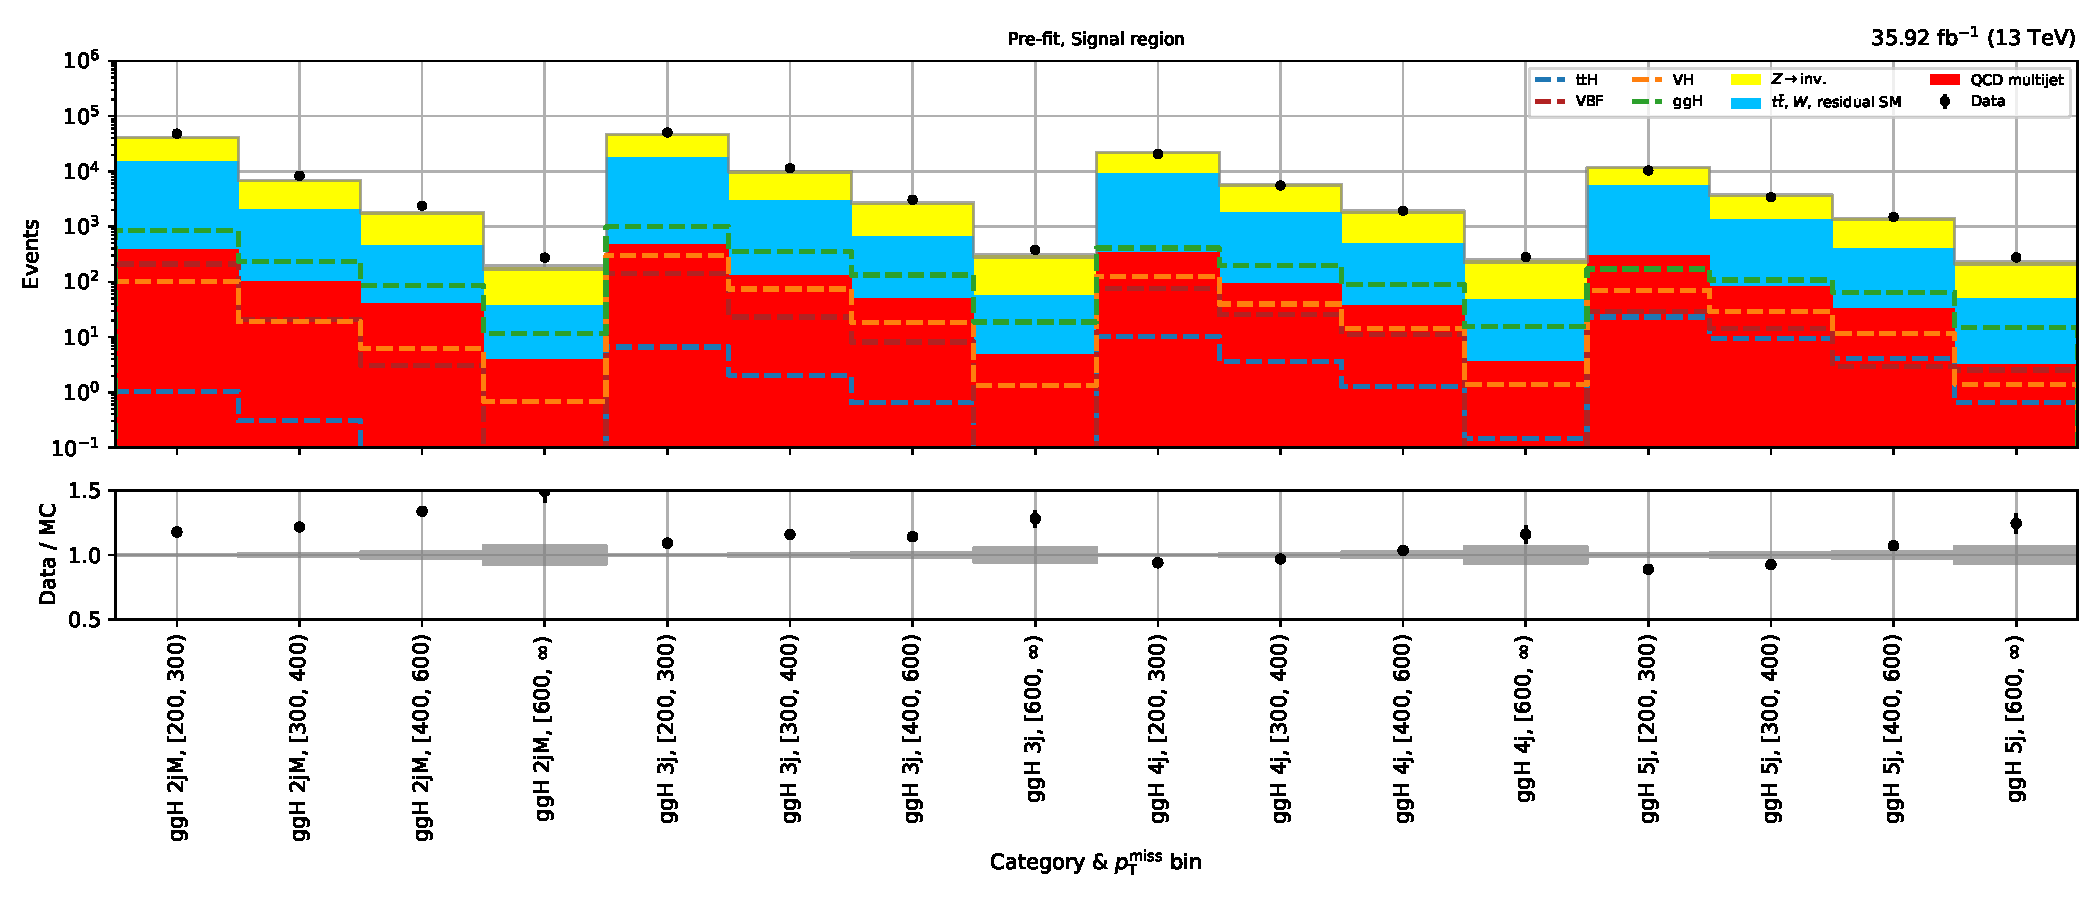
\includegraphics[width=\textwidth]{figures/mountain_ranges/2016/ggF/SR_tree_prefit-abs_values_ggF_cats.pdf}
        \caption{\ggH --- 2016 (pre-fit)}
    \end{subfigure}

    \begin{subfigure}[b]{0.9\textwidth}
        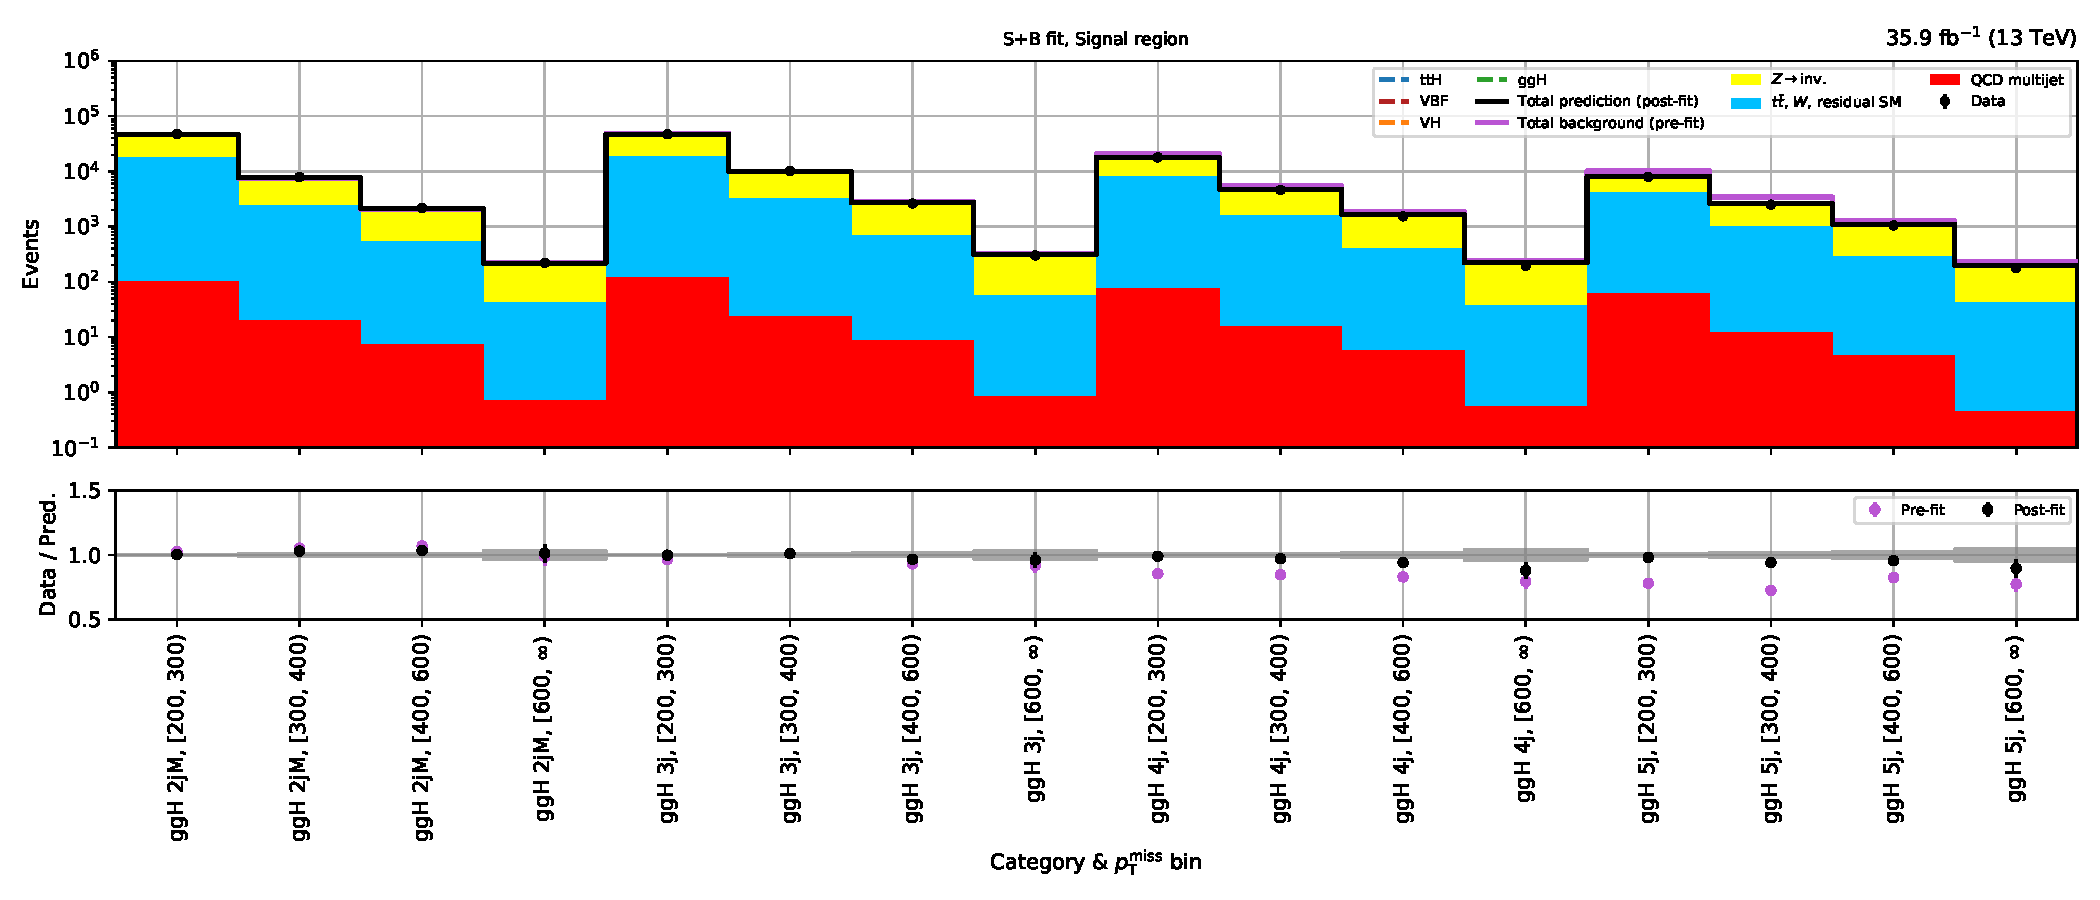
\includegraphics[width=\textwidth]{figures/mountain_ranges/2016/ggF/SR_tree_fit_s-abs_values_ggF_cats.pdf}
        \caption{\ggH --- 2016 (post-fit)}
    \end{subfigure}
    \caption[Pre-fit and post-fit yields for each \ggH subcategory and \ptmiss bin for the 2016 dataset]{Pre-fit and post-fit yields for each \ggH subcategory and \ptmiss bin for the 2016 dataset. In bottom panel of post-fit plot, the ratio data to signal plus background is calculated.}
    \label{fig:htoinv_mountain_range_ggH_2016}
\end{figure}

\begin{figure}[htbp]
    \centering
    \begin{subfigure}[b]{0.9\textwidth}
        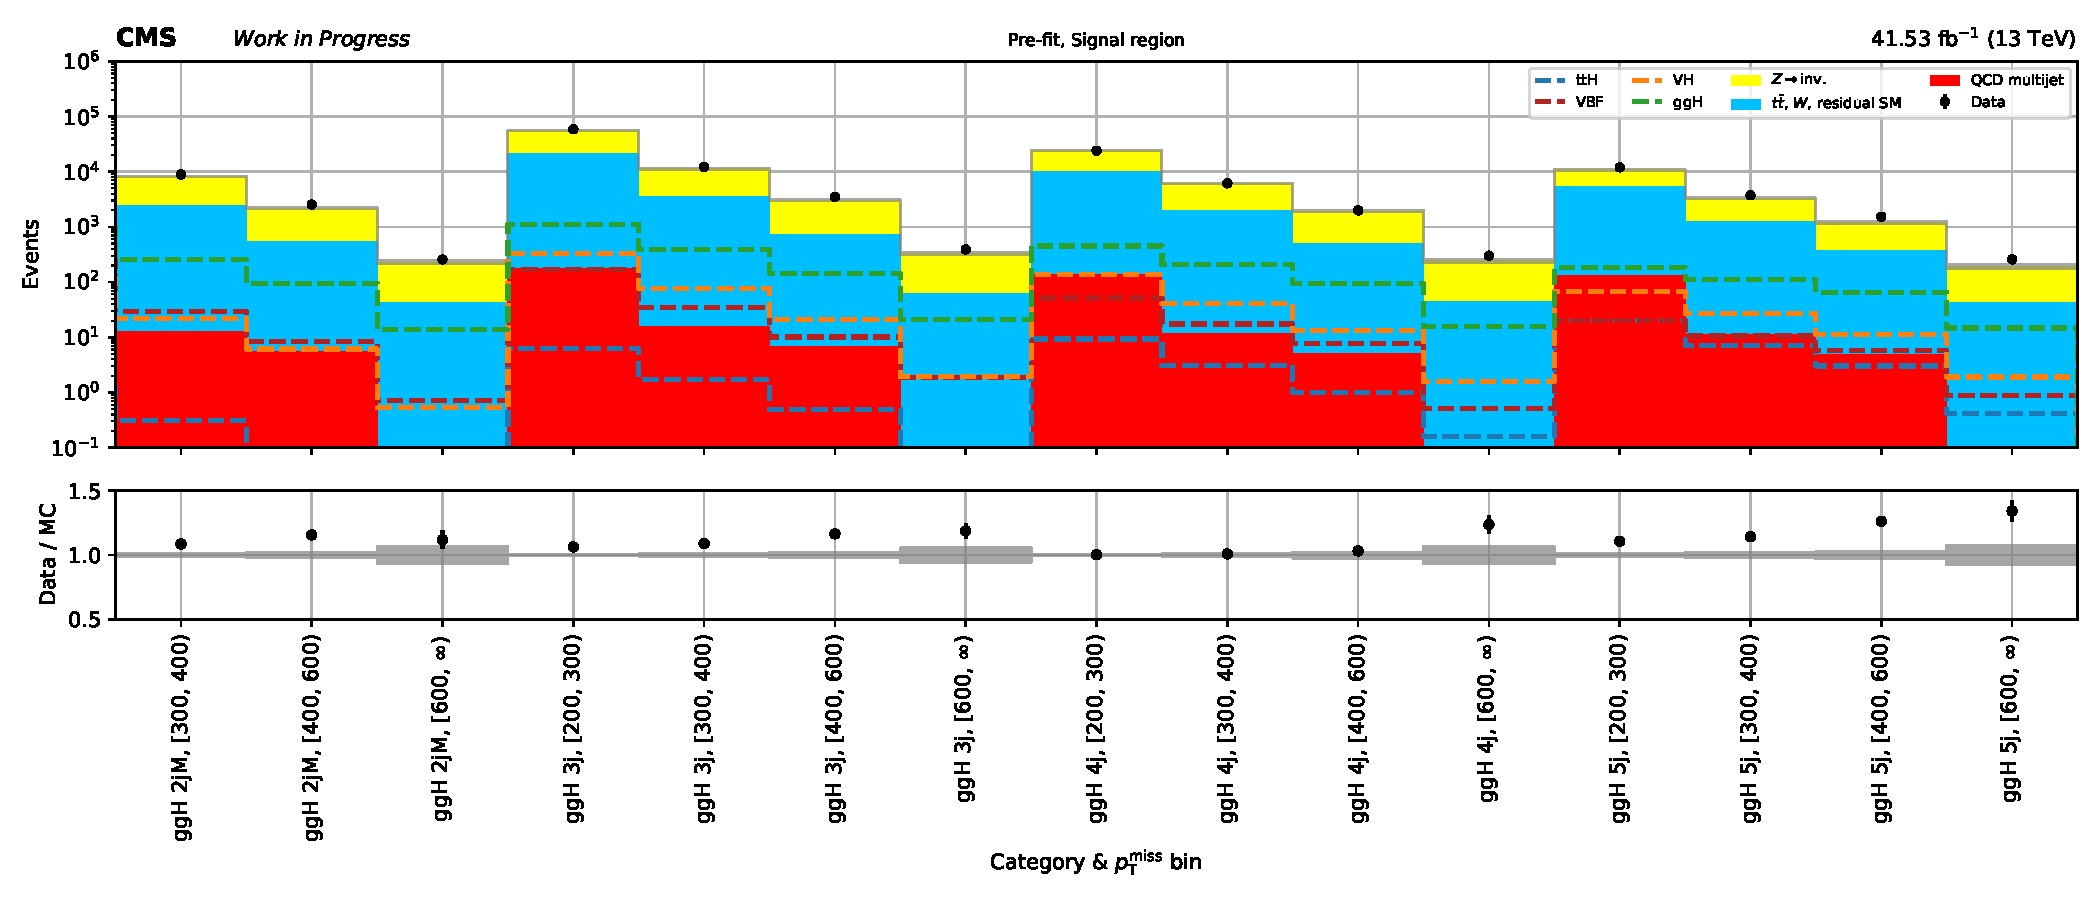
\includegraphics[width=\textwidth]{figures/mountain_ranges/2017/ggF/SR_tree_prefit-abs_values_ggF_cats.pdf}
        \caption{\ggH --- 2017 (pre-fit)}
    \end{subfigure}

    \begin{subfigure}[b]{0.9\textwidth}
        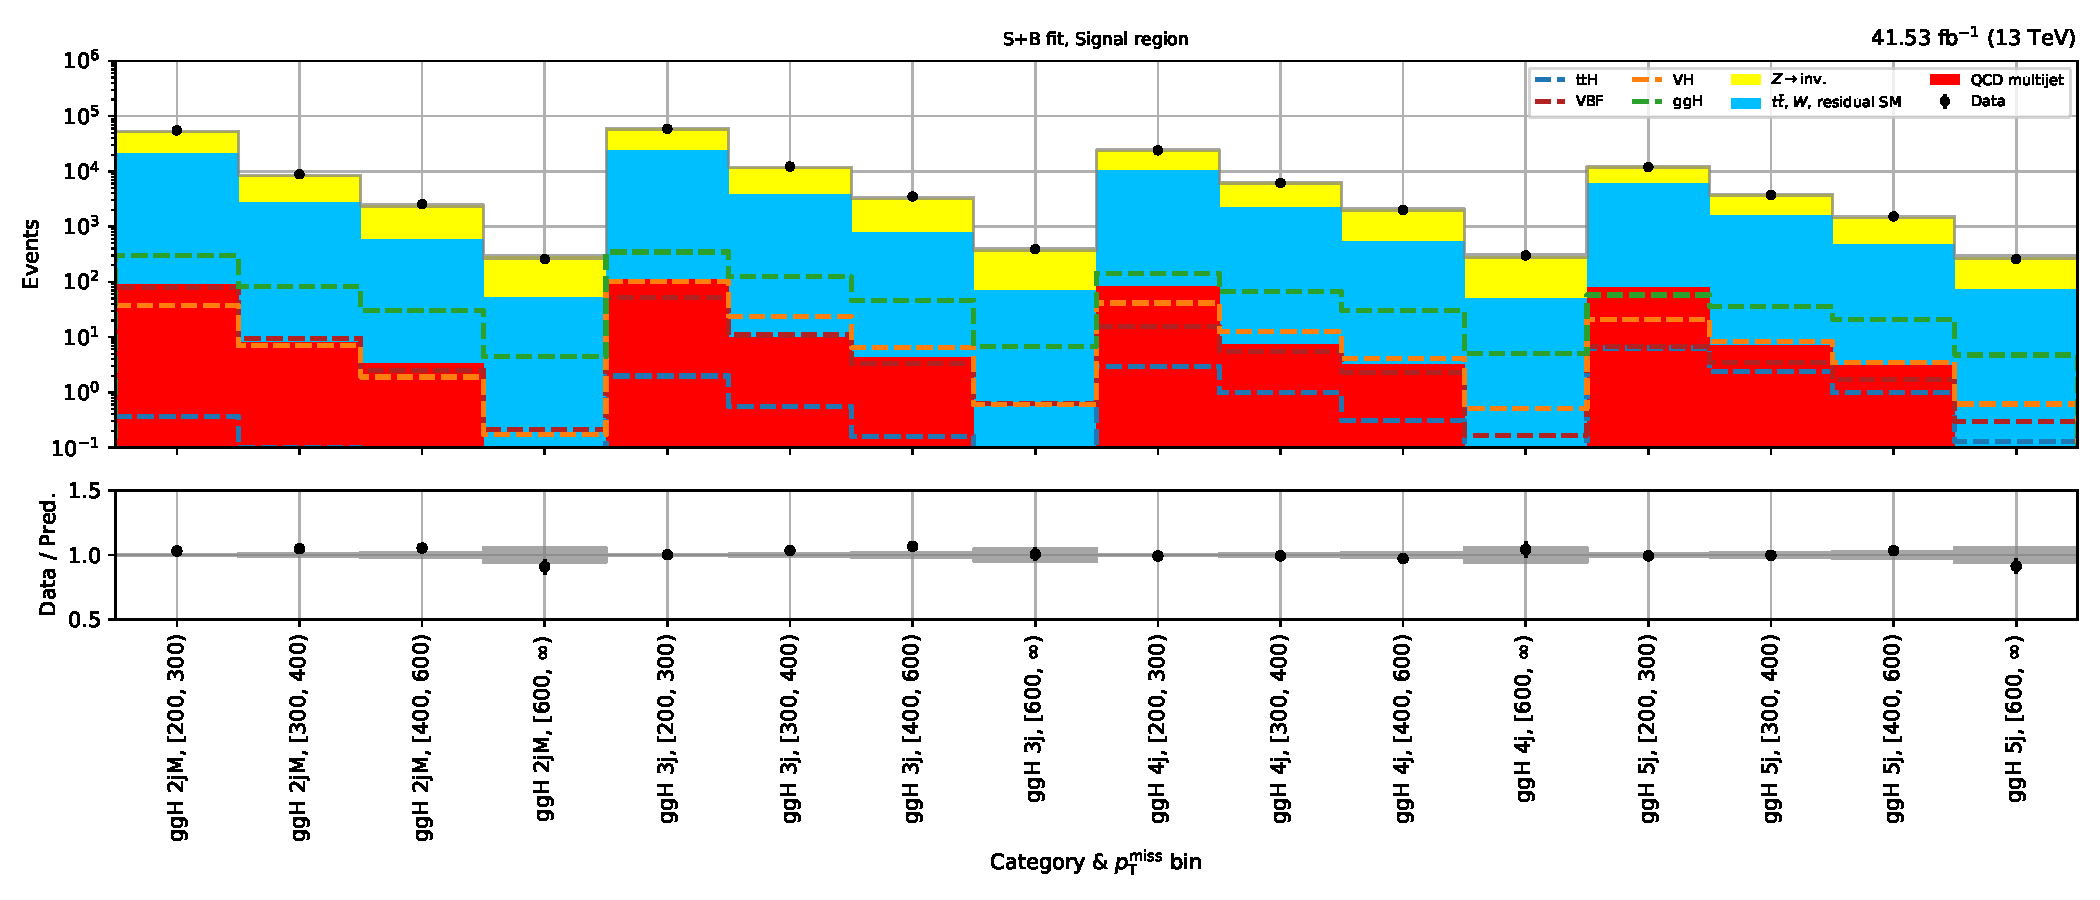
\includegraphics[width=\textwidth]{figures/mountain_ranges/2017/ggF/SR_tree_fit_s-abs_values_ggF_cats.pdf}
        \caption{\ggH --- 2017 (post-fit)}
    \end{subfigure}
    \caption[Pre-fit and post-fit yields for each \ggH subcategory and \ptmiss bin for the 2017 dataset]{Pre-fit and post-fit yields for each \ggH subcategory and \ptmiss bin for the 2017 dataset. In bottom panel of post-fit plot, the ratio data to signal plus background is calculated.}
    \label{fig:htoinv_mountain_range_ggH_2017}
\end{figure}

\begin{figure}[htbp]
    \centering
    \begin{subfigure}[b]{0.9\textwidth}
        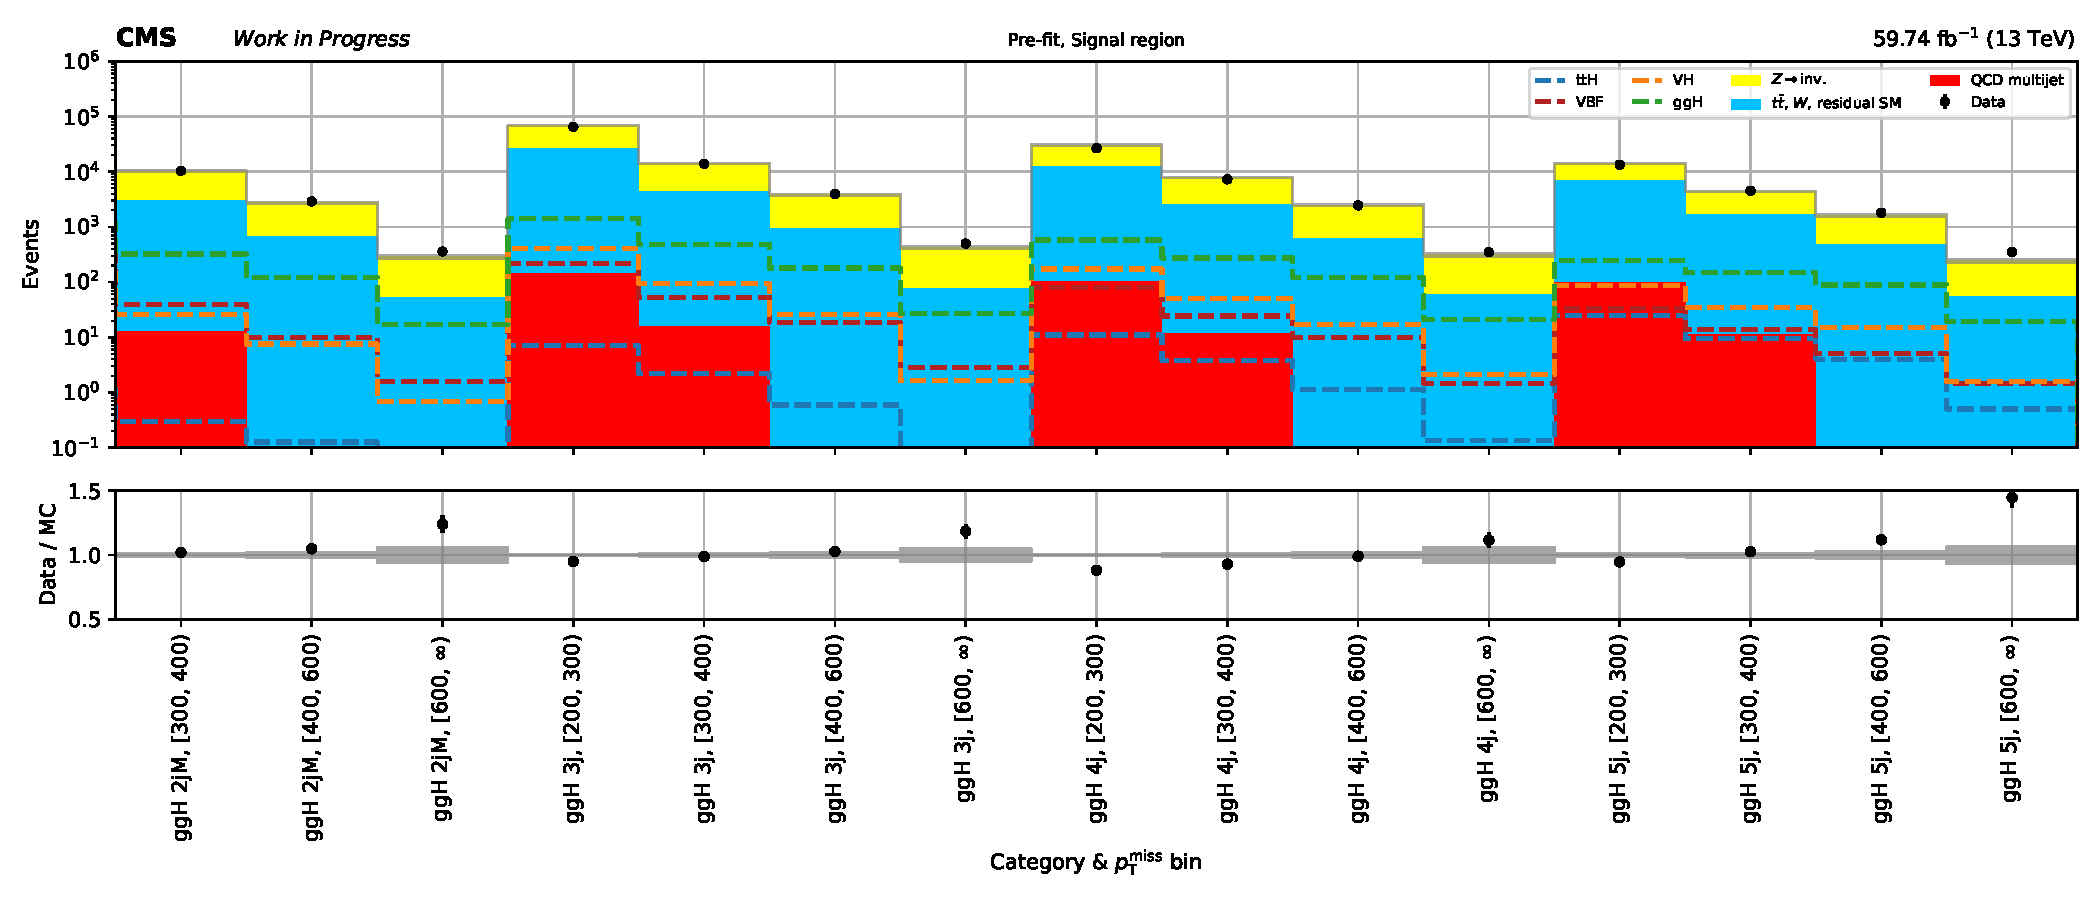
\includegraphics[width=\textwidth]{figures/mountain_ranges/2018/ggF/SR_tree_prefit-abs_values_ggF_cats.pdf}
        \caption{\ggH --- 2018 (pre-fit)}
    \end{subfigure}

    \begin{subfigure}[b]{0.9\textwidth}
        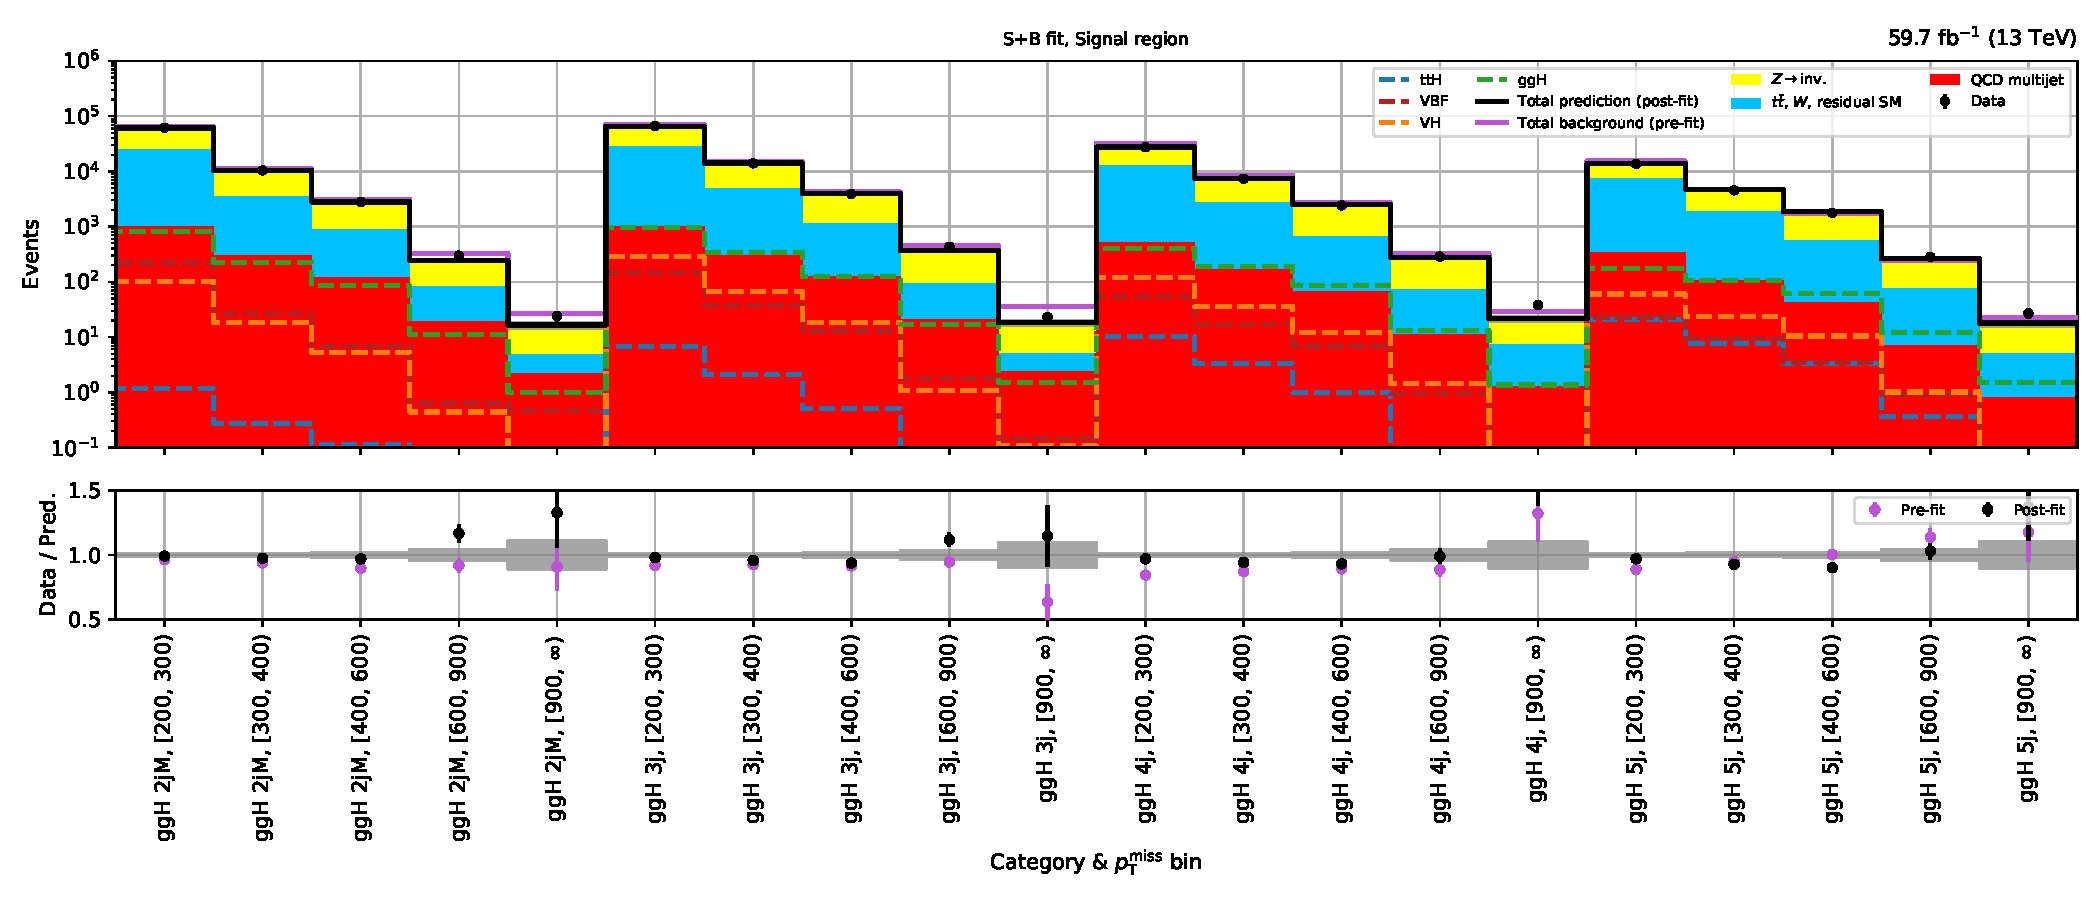
\includegraphics[width=\textwidth]{figures/mountain_ranges/2018/ggF/SR_tree_fit_s-abs_values_ggF_cats.pdf}
        \caption{\ggH --- 2018 (post-fit)}
    \end{subfigure}
    \caption[Pre-fit and post-fit yields for each \ggH subcategory and \ptmiss bin for the 2018 dataset]{Pre-fit and post-fit yields for each \ggH subcategory and \ptmiss bin for the 2018 dataset. In bottom panel of post-fit plot, the ratio data to signal plus background is calculated.}
    \label{fig:htoinv_mountain_range_ggH_2018}
\end{figure}

\clearpage


%=========================================================


\section{Combined results}
\label{sec:htoinv_combined_results}

% Show the results combined over all production modes (one plot for each year), then the full combination for Run-2, ideally with VBF results as well

Upper limits for $\BRof{\higgstoinv}$ by combining all categories for a given year are given for 2016, 2017, and 2018 in Figs.~\ref{fig:htoinv_limit_likelihood_2016}, \ref{fig:htoinv_limit_likelihood_2017}, \ref{fig:htoinv_limit_likelihood_2018}, respectively. For the full Run-2 dataset, they are broken down by data taking year in Fig.~\ref{fig:htoinv_limit_likelihood_Run2_per_year} and by category in Fig.~\ref{fig:htoinv_limit_likelihood_Run2_per_cat}.\footnote{Expected limits only, so far, and really only placeholders. The full Run-2 likelihood is not correct---fit fails to converge for most points.} Profile likelihood ratios as a function of $\BRof{\higgstoinv}$ are also presented opposite the limits.

\begin{figure}[htbp]
    \centering
    \begin{subfigure}[t]{0.45\textwidth}  % top align since figures are same dimensions, but x-axis labels are larger for likelihood
        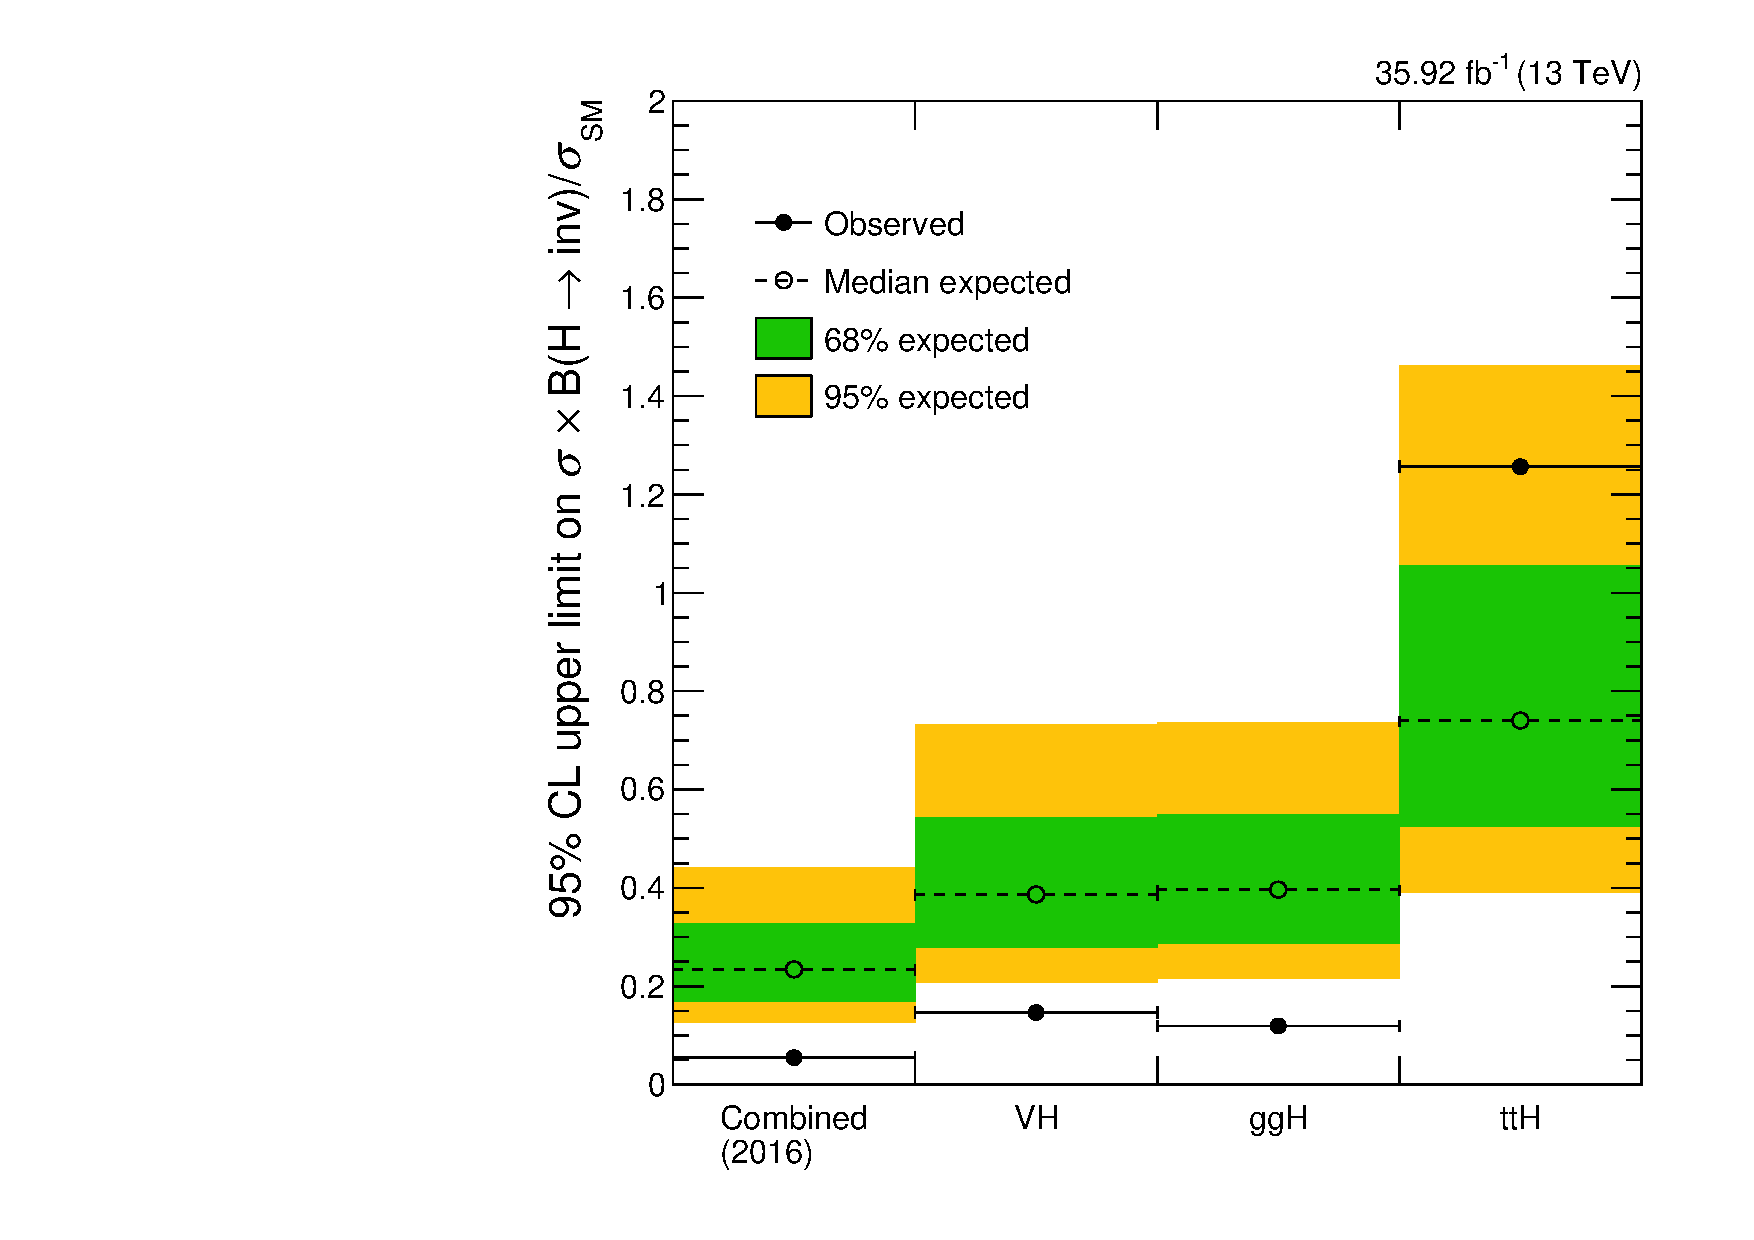
\includegraphics[width=\textwidth]{figures/limits/per_year/limit_2016_comb.pdf}
        \caption{Limit -- 2016}
    \end{subfigure}
    \hspace{0.05\textwidth}
    \begin{subfigure}[t]{0.45\textwidth}
        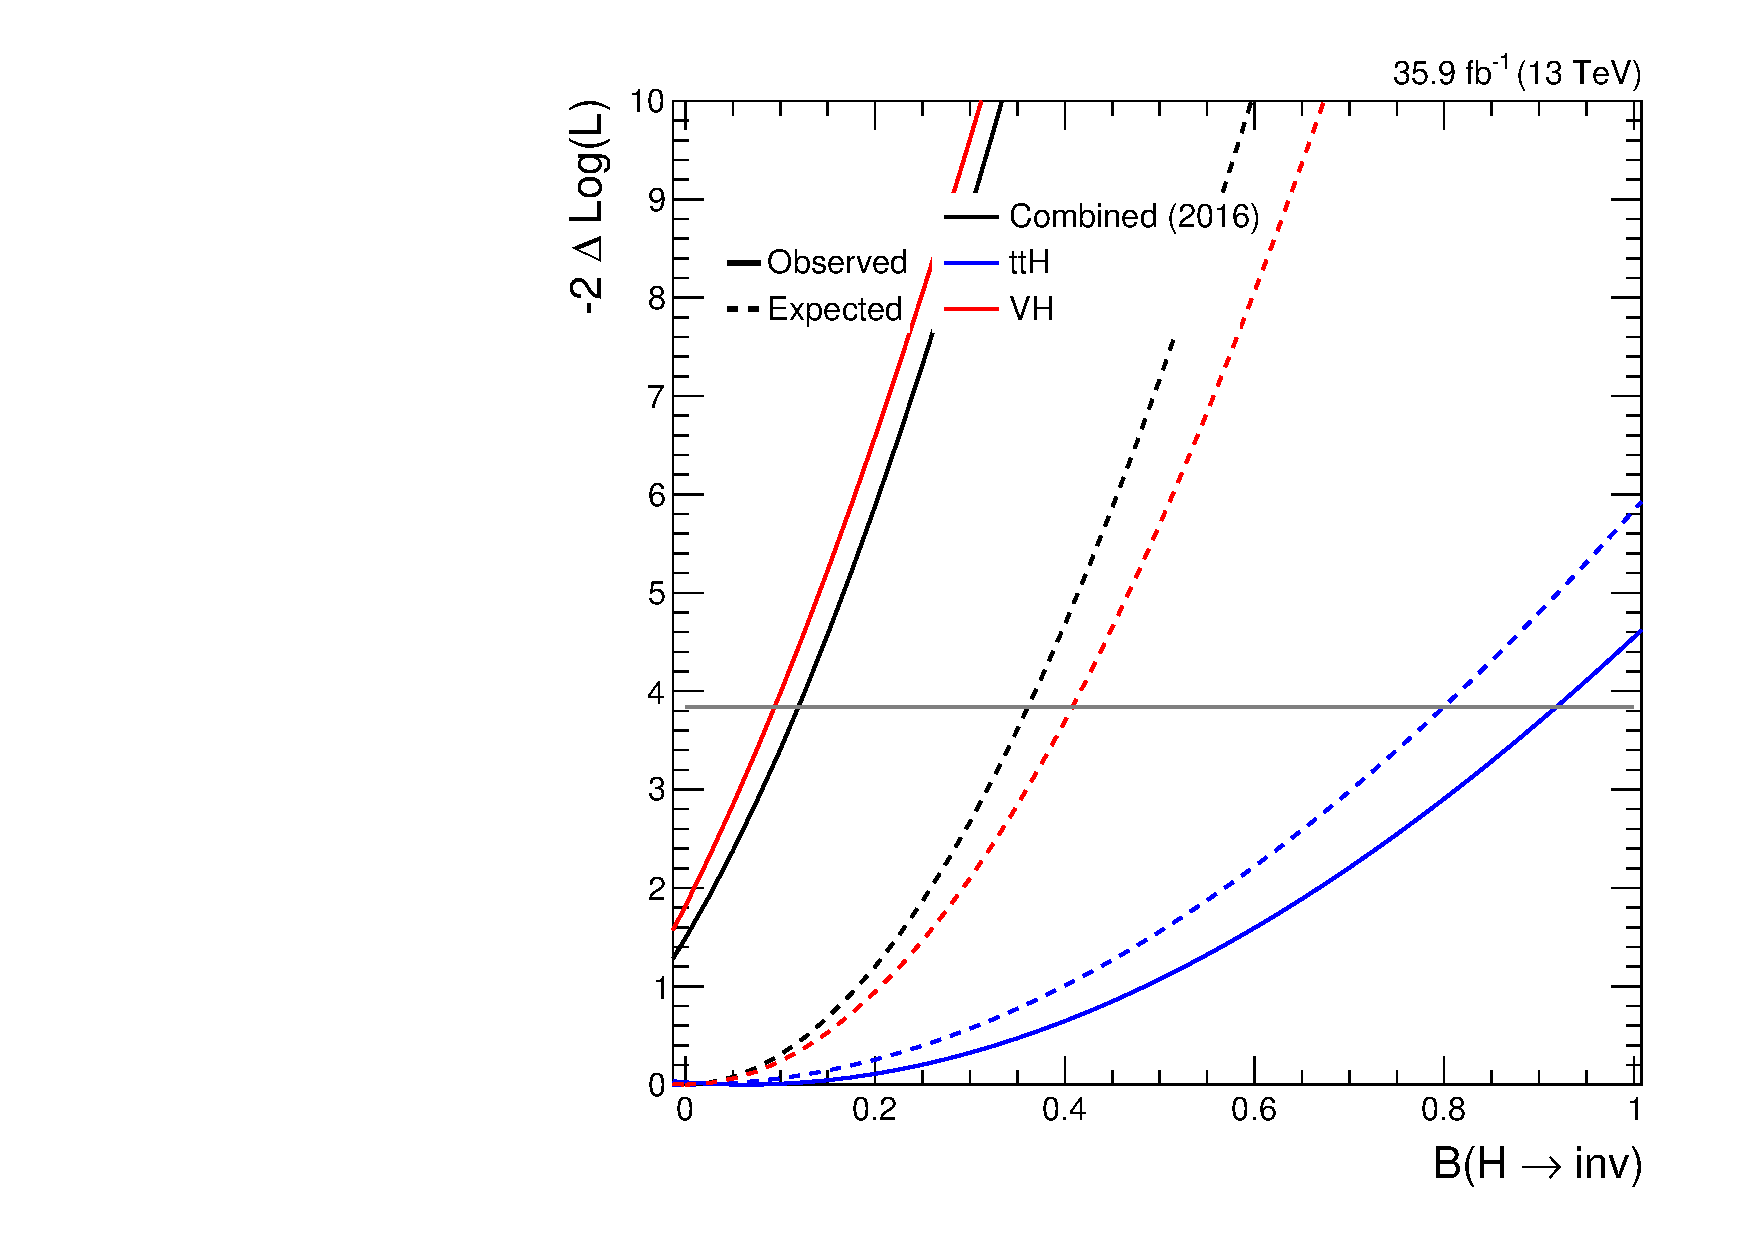
\includegraphics[width=\textwidth]{figures/likelihood_scan/profile_likelihood_scan_2016.pdf}
        \caption{Profile likelihood -- 2016}
    \end{subfigure}
    \caption[Observed and expected 95\,\% CL upper limit on the Higgs boson to invisible state branching fraction $\BRof{\higgstoinv}$ and the corresponding profile likelihood ratio as a function of it, for both the individual categories that target a specific production mode, as well as the combination of them, for the 2016 dataset]{Observed and expected 95\,\% CL upper limit on the Higgs boson to invisible state branching fraction $\BRof{\higgstoinv}$ (left) and the corresponding profile likelihood ratio as a function of it (right), for both the individual categories that target a specific production mode, as well as the combination of them, for the 2016 dataset. The \acrlong{sm} Higgs boson with its associated mass and production cross section are assumed.}
    \label{fig:htoinv_limit_likelihood_2016}
\end{figure}

\begin{figure}[htbp]
    \centering
    \begin{subfigure}[t]{0.45\textwidth}
        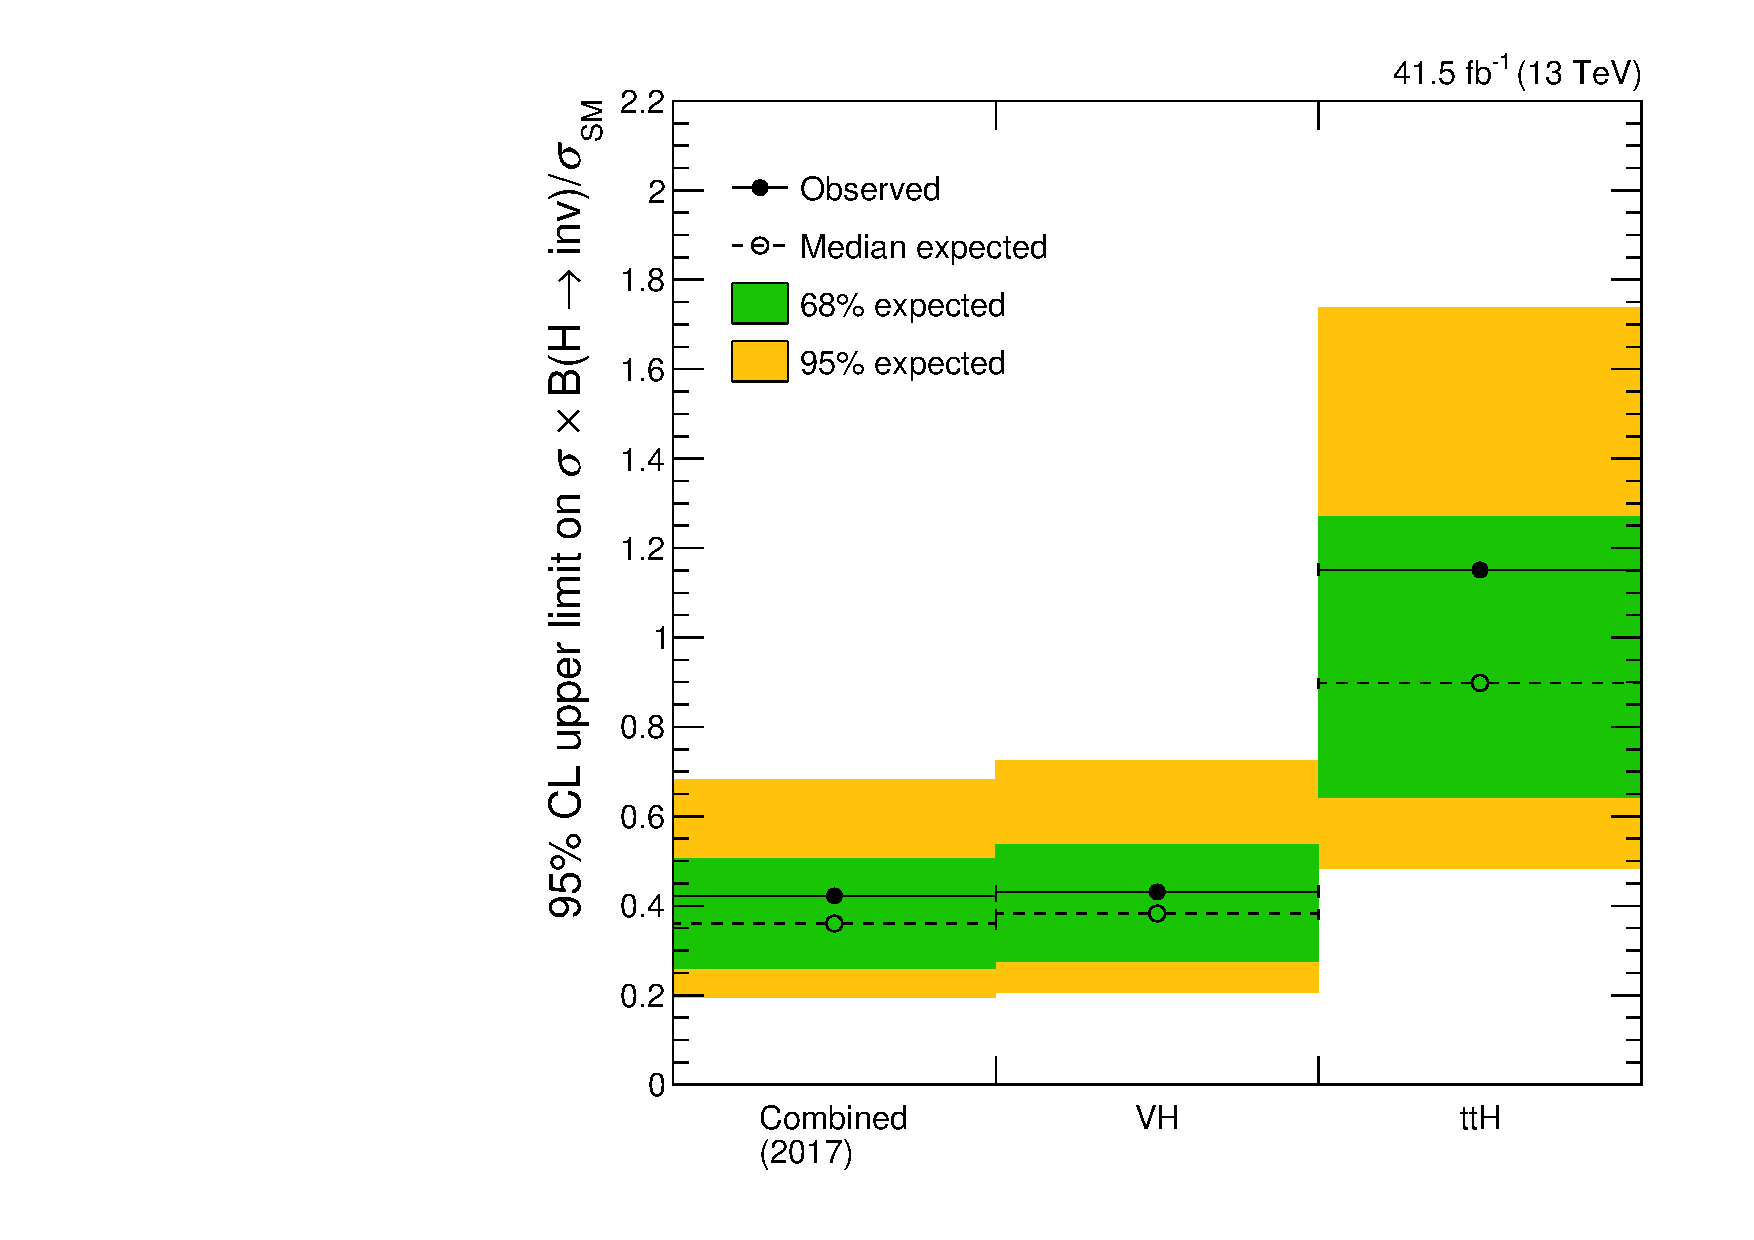
\includegraphics[width=\textwidth]{figures/limits/per_year/limit_2017_comb.pdf}
        \caption{Limit -- 2017}
    \end{subfigure}
    \hspace{0.05\textwidth}
    \begin{subfigure}[t]{0.45\textwidth}
        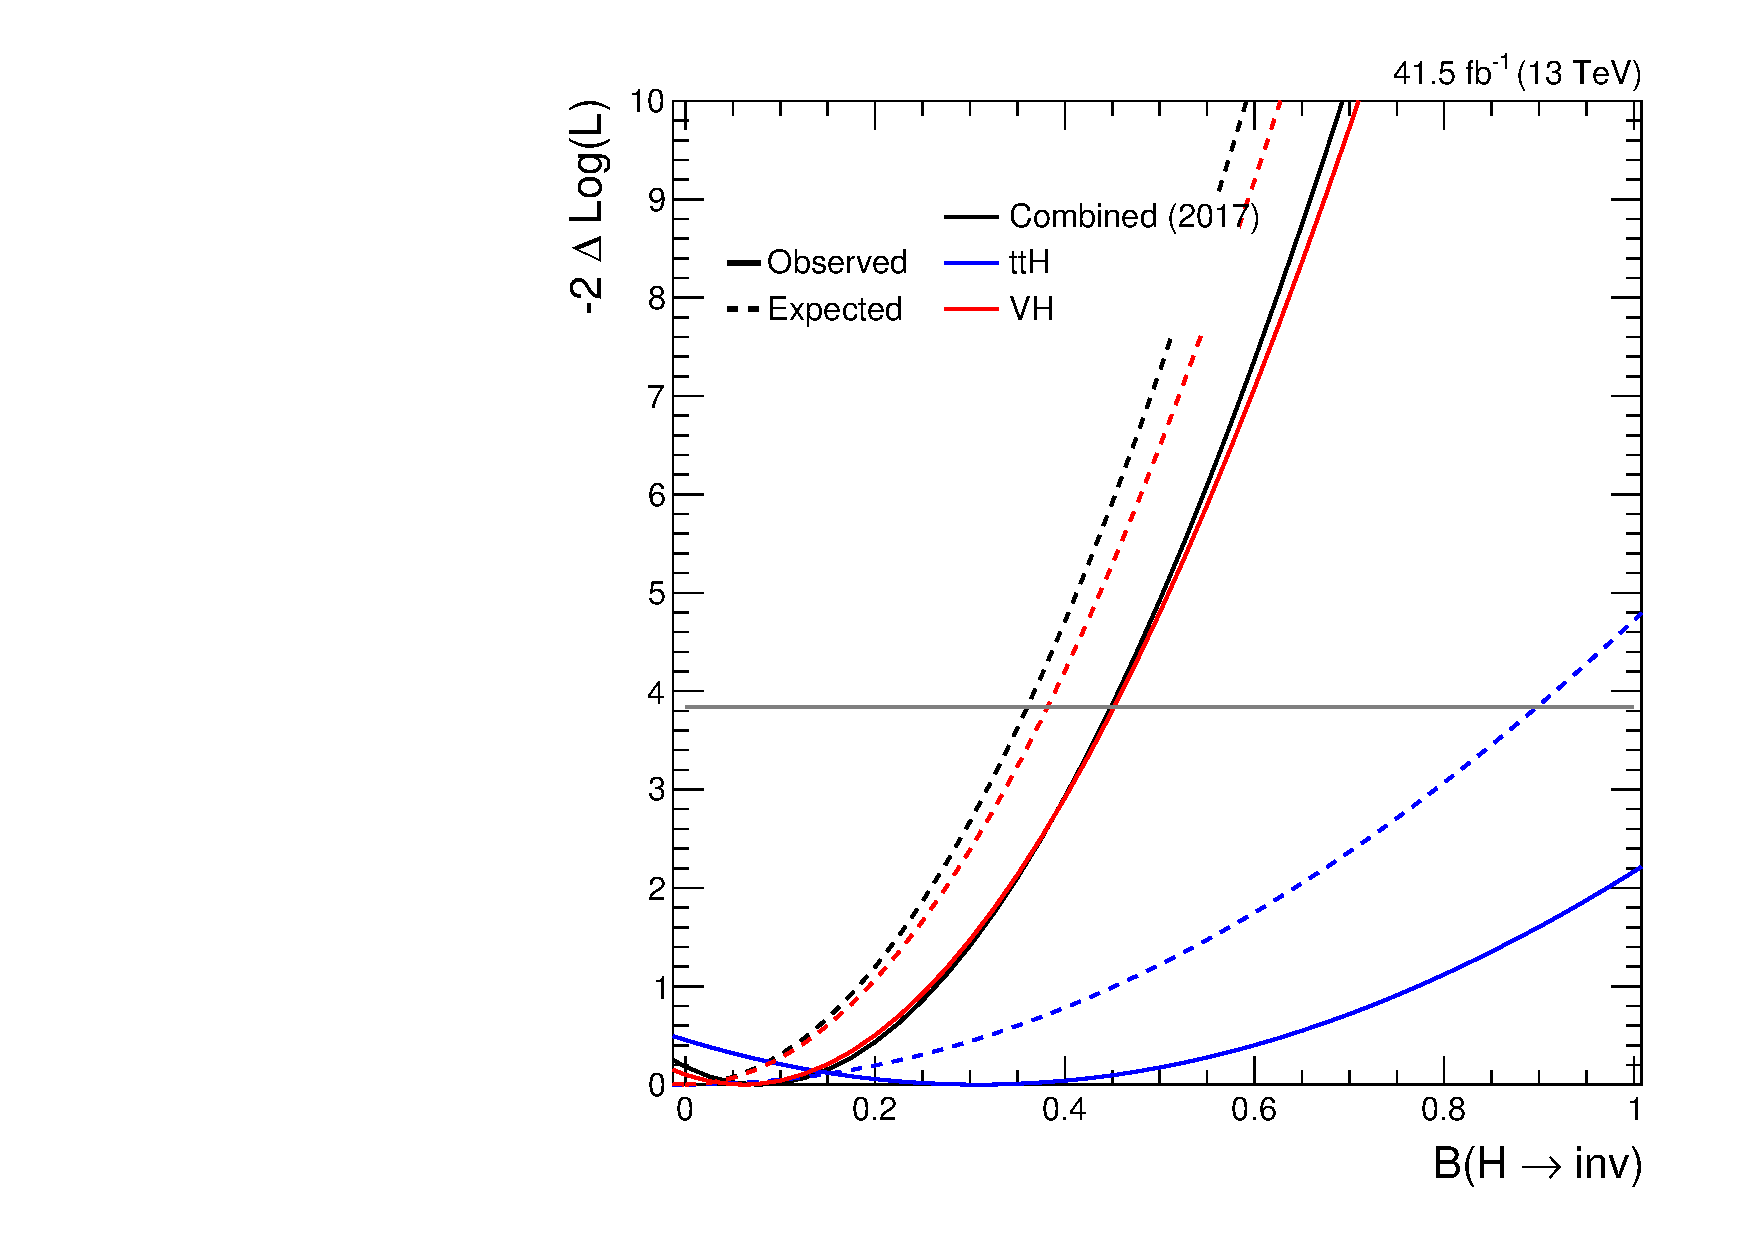
\includegraphics[width=\textwidth]{figures/likelihood_scan/profile_likelihood_scan_2017.pdf}
        \caption{Profile likelihood -- 2017}
    \end{subfigure}
    \caption[Observed and expected 95\,\% CL upper limit on the Higgs boson to invisible state branching fraction $\BRof{\higgstoinv}$ and the corresponding profile likelihood ratio as a function of it, for both the individual categories that target a specific production mode, as well as the combination of them, for the 2017 dataset]{Observed and expected 95\,\% CL upper limit on the Higgs boson to invisible state branching fraction $\BRof{\higgstoinv}$ (left) and the corresponding profile likelihood ratio as a function of it (right), for both the individual categories that target a specific production mode, as well as the combination of them, for the 2017 dataset. The \acrlong{sm} Higgs boson with its associated mass and production cross section are assumed.}
    \label{fig:htoinv_limit_likelihood_2017}
\end{figure}

\begin{figure}[htbp]
    \centering
    \begin{subfigure}[t]{0.45\textwidth}
        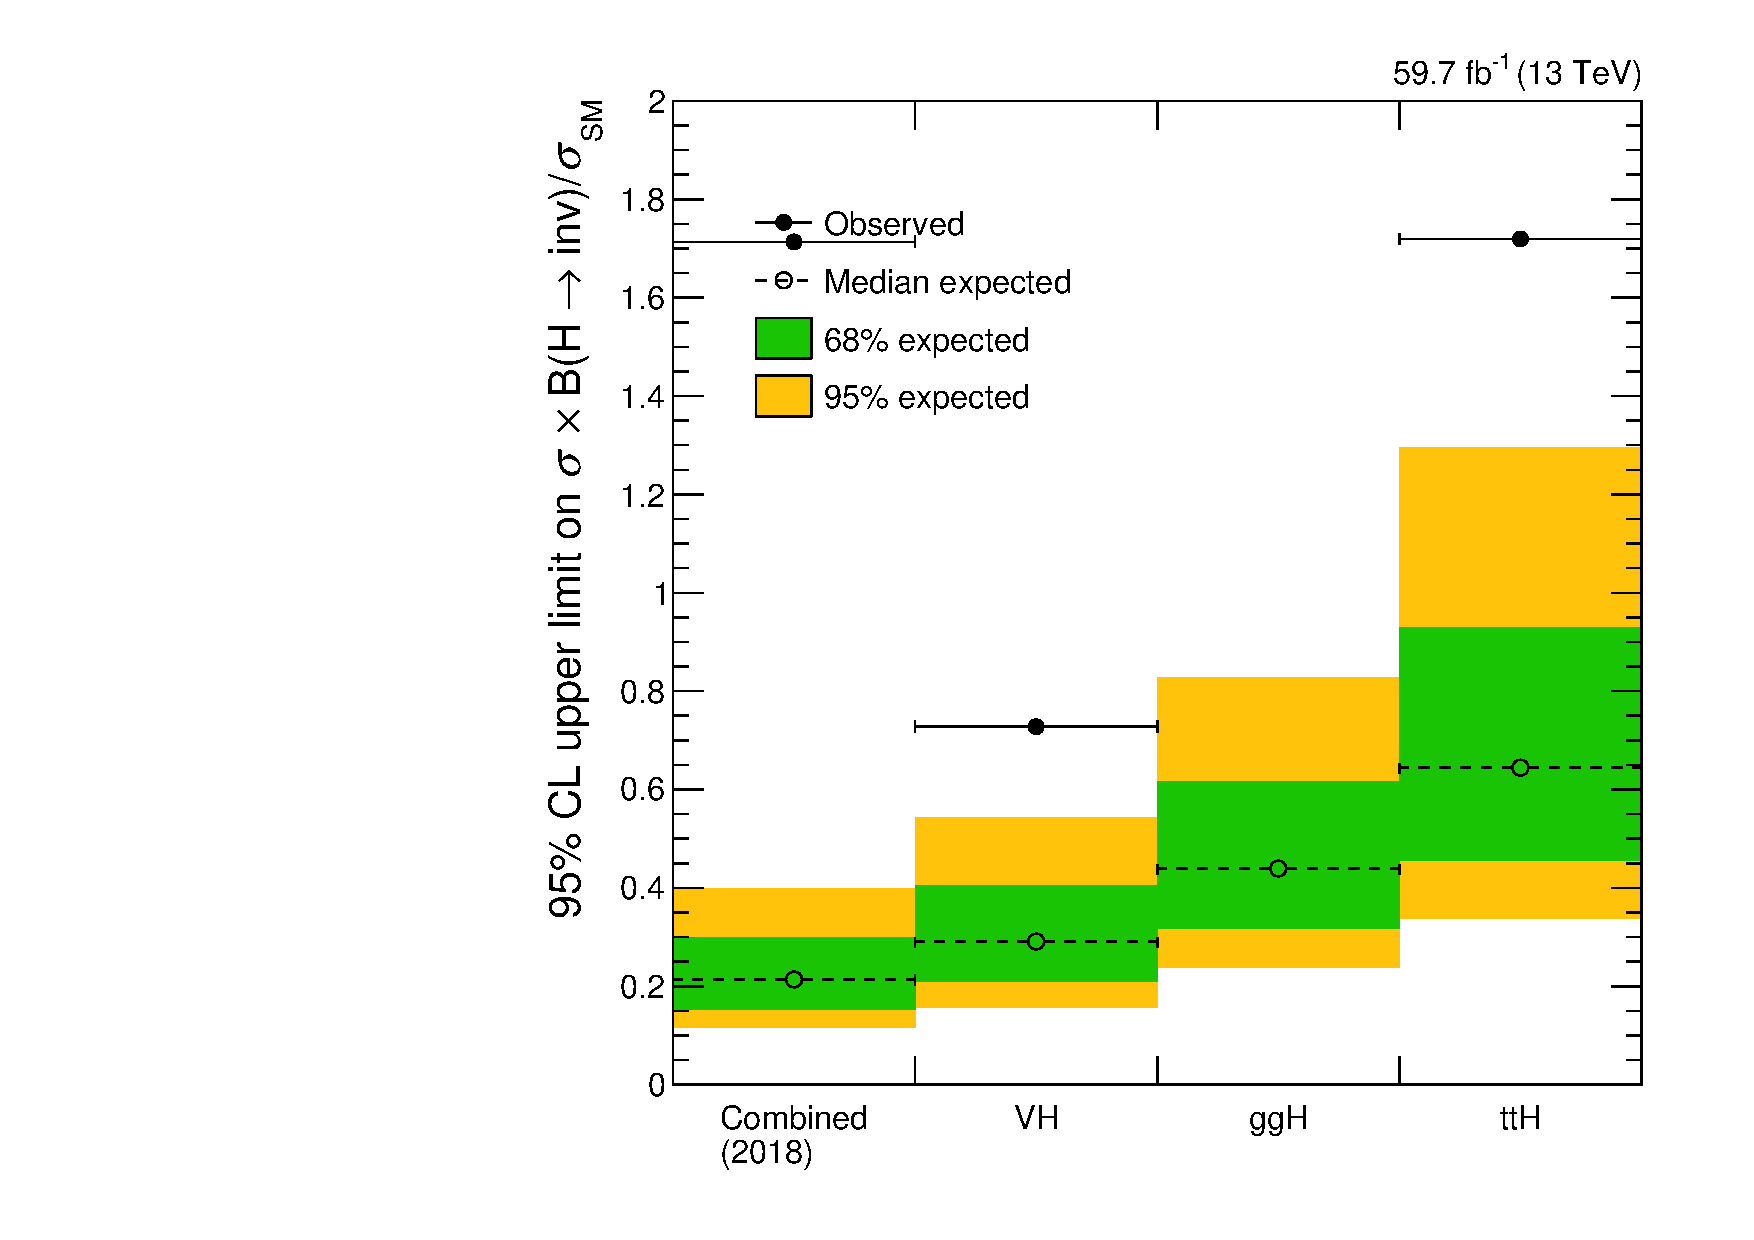
\includegraphics[width=\textwidth]{figures/limits/per_year/limit_2018_comb.pdf}
        \caption{Limit -- 2018}
    \end{subfigure}
    \hspace{0.05\textwidth}
    \begin{subfigure}[t]{0.45\textwidth}
        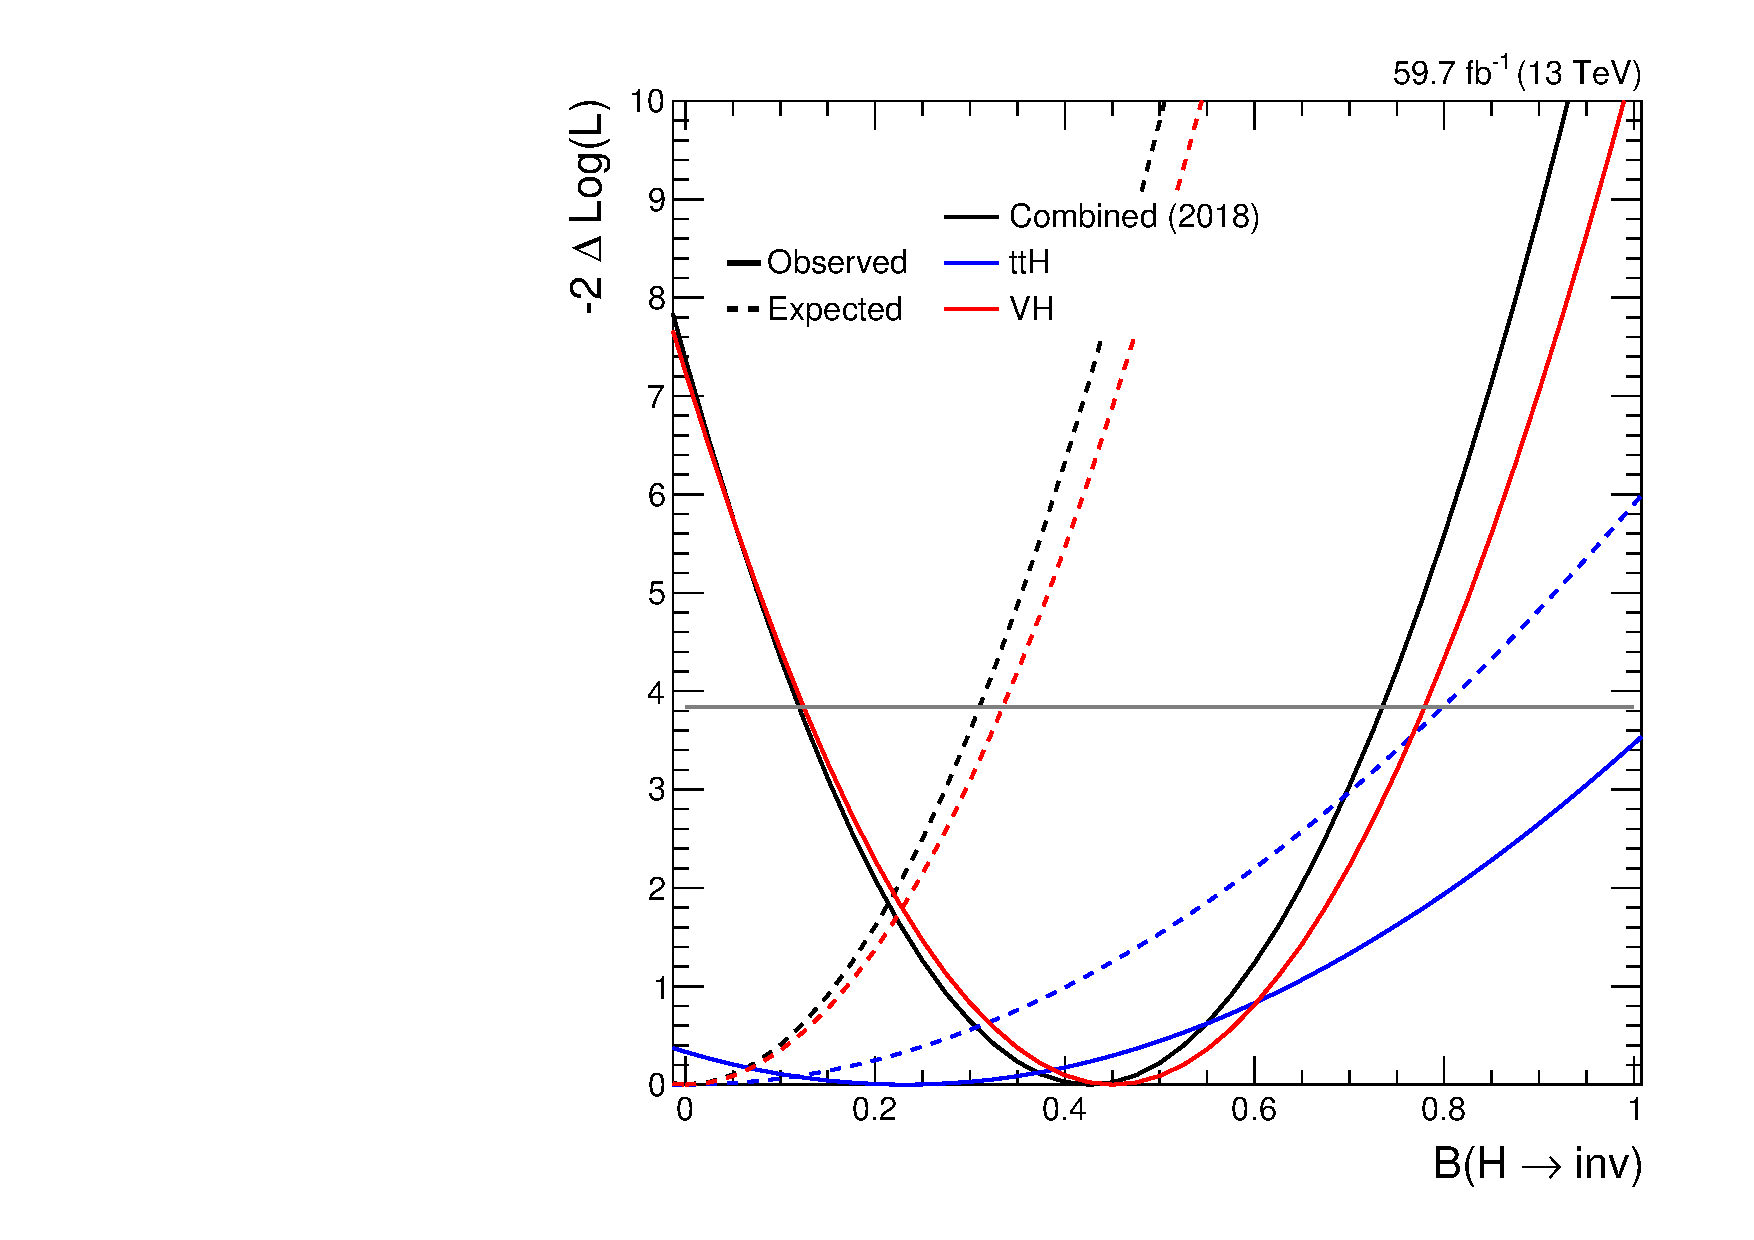
\includegraphics[width=\textwidth]{figures/likelihood_scan/profile_likelihood_scan_2018.pdf}
        \caption{Profile likelihood -- 2018}
    \end{subfigure}
    \caption[Observed and expected 95\,\% CL upper limit on the Higgs boson to invisible state branching fraction $\BRof{\higgstoinv}$ and the corresponding profile likelihood ratio as a function of it, for both the individual categories that target a specific production mode, as well as the combination of them, for the 2018 dataset]{Observed and expected 95\,\% CL upper limit on the Higgs boson to invisible state branching fraction $\BRof{\higgstoinv}$ (left) and the corresponding profile likelihood ratio as a function of it (right), for both the individual categories that target a specific production mode, as well as the combination of them, for the 2018 dataset. The \acrlong{sm} Higgs boson with its associated mass and production cross section are assumed.}
    \label{fig:htoinv_limit_likelihood_2018}
\end{figure}

\begin{figure}[htbp]
    \centering
    \begin{subfigure}[t]{0.45\textwidth}
        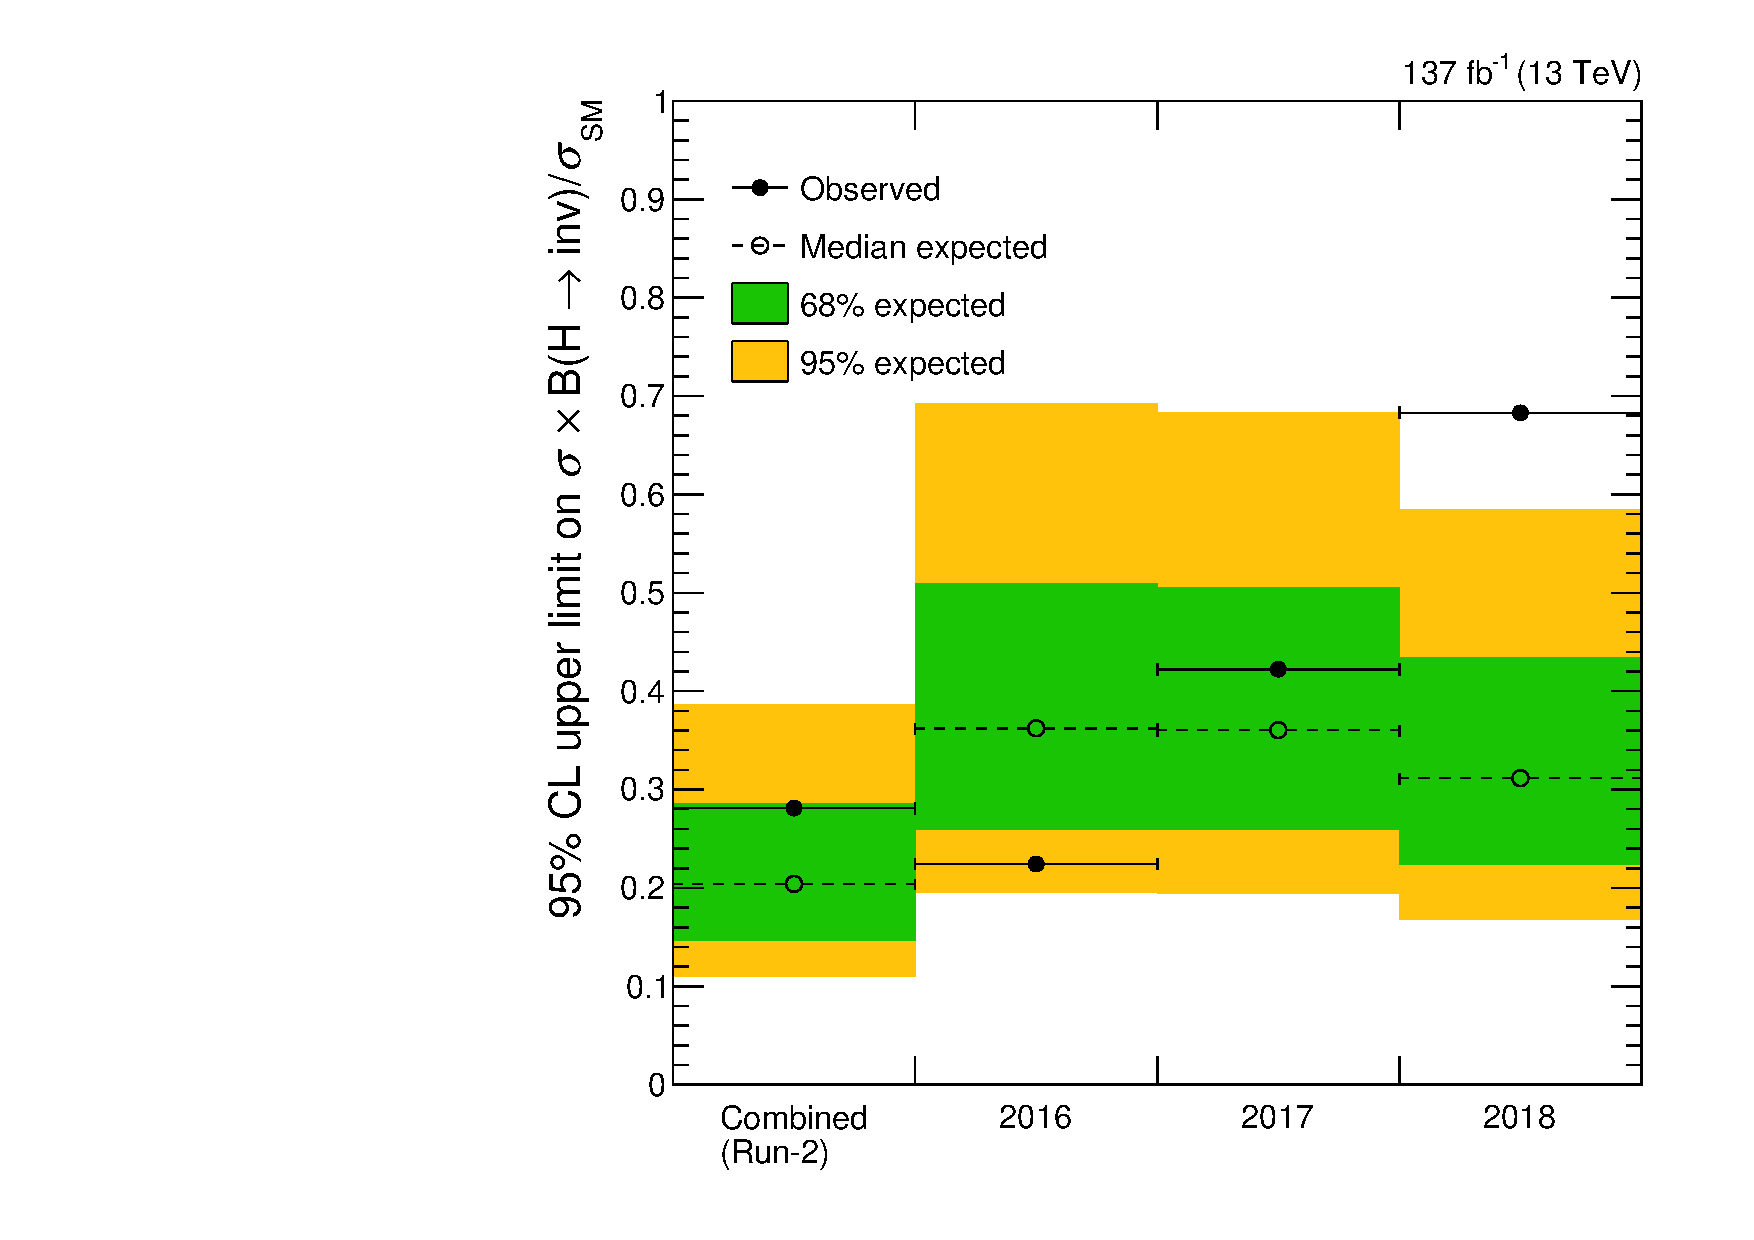
\includegraphics[width=\textwidth]{figures/limits/full_Run2/limit_Run2_comb_per_year.pdf}
        \caption{Limit -- Run-2}
    \end{subfigure}
    \hspace{0.05\textwidth}
    \begin{subfigure}[t]{0.45\textwidth}
        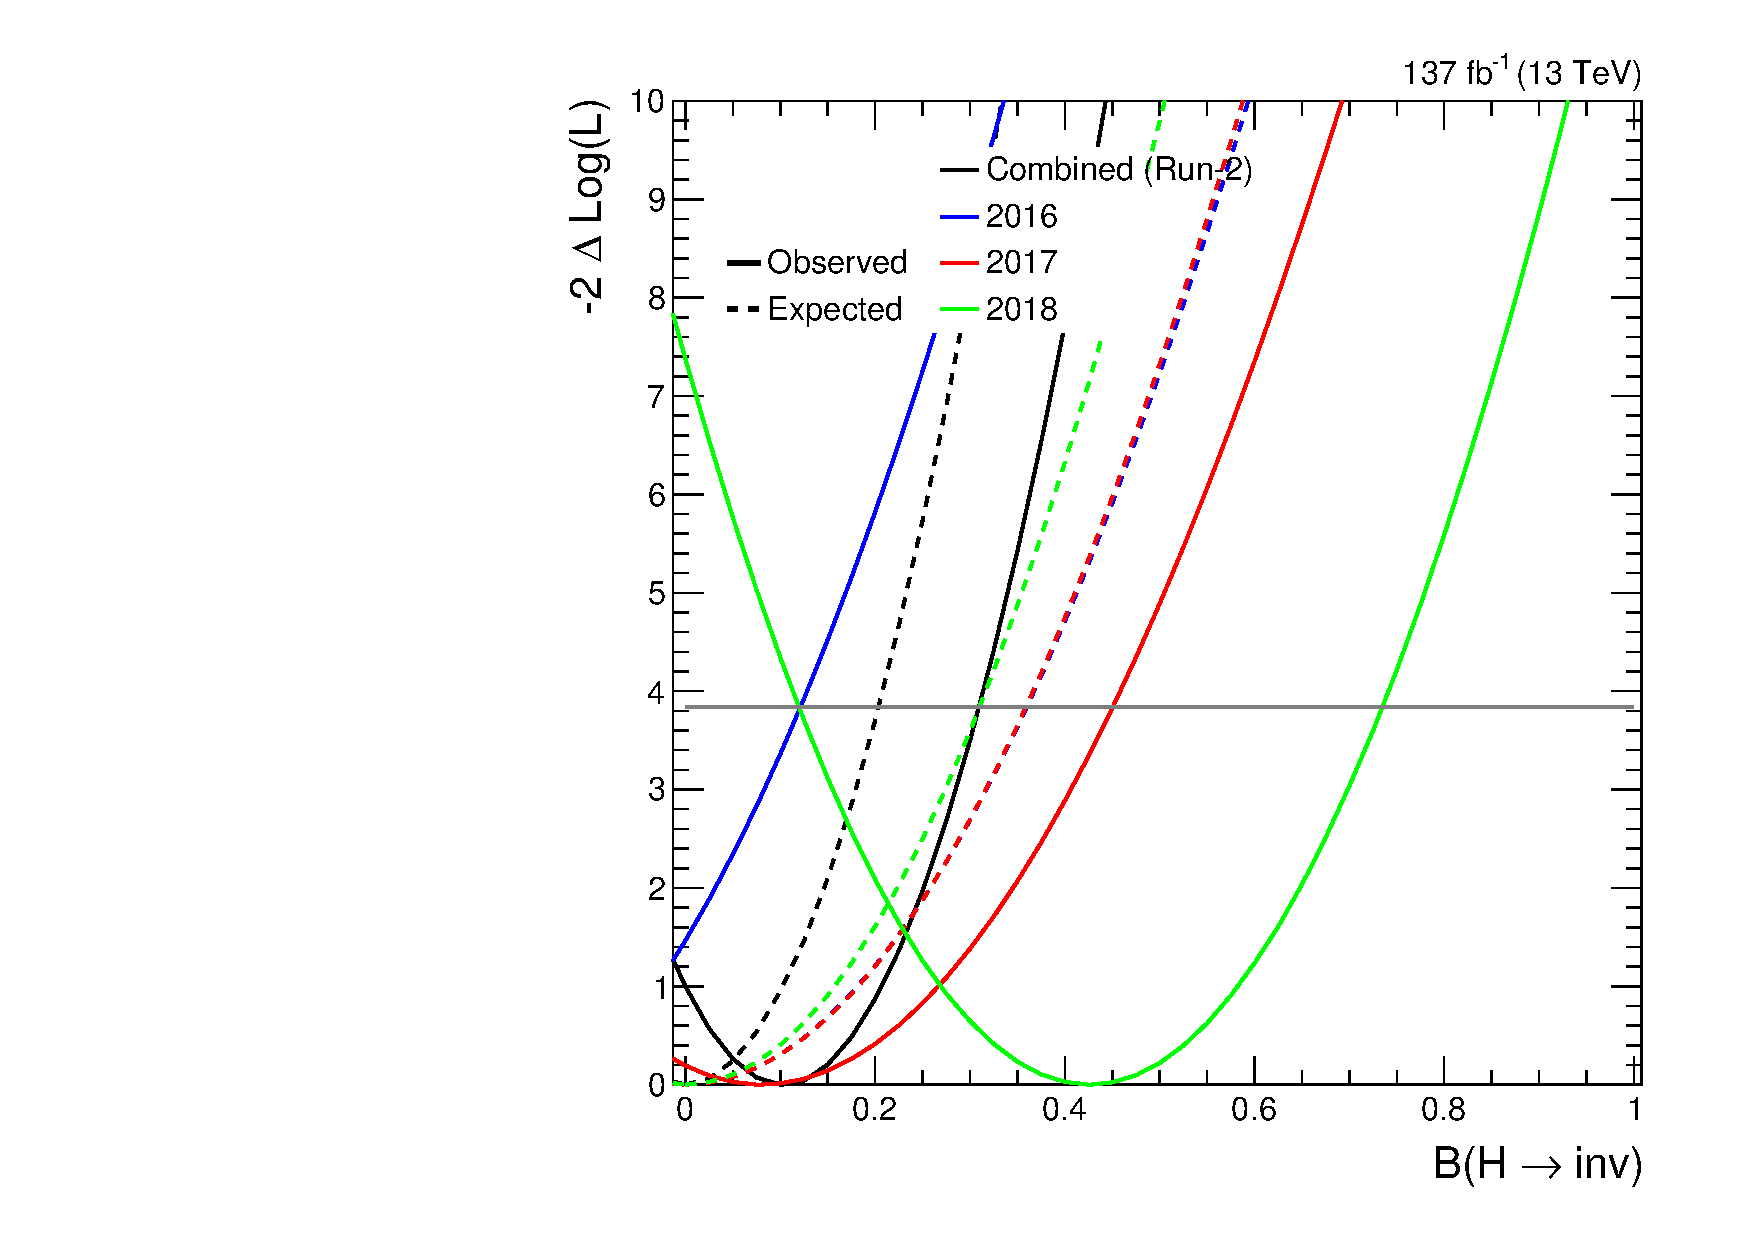
\includegraphics[width=\textwidth]{figures/likelihood_scan/profile_likelihood_scan_Run2_per_year.pdf}
        \caption{Profile likelihood -- Run-2}
    \end{subfigure}
    \caption[Observed and expected 95\,\% CL upper limit on the Higgs boson to invisible state branching fraction $\BRof{\higgstoinv}$ and the corresponding profile likelihood ratio as a function of it, for both the individual data taking years, as well as the combination of them, for the full Run-2 dataset]{Observed and expected 95\,\% CL upper limit on the Higgs boson to invisible state branching fraction $\BRof{\higgstoinv}$ (left) and the corresponding profile likelihood ratio as a function of it (right), for both the individual data taking years, as well as the combination of them, for the full Run-2 dataset. The \acrlong{sm} Higgs boson with its associated mass and production cross section are assumed.}
    \label{fig:htoinv_limit_likelihood_Run2_per_year}
\end{figure}

\begin{figure}[htbp]
    \centering
    \begin{subfigure}[b]{0.45\textwidth}  % top align since axis labels are larger for likelihood
        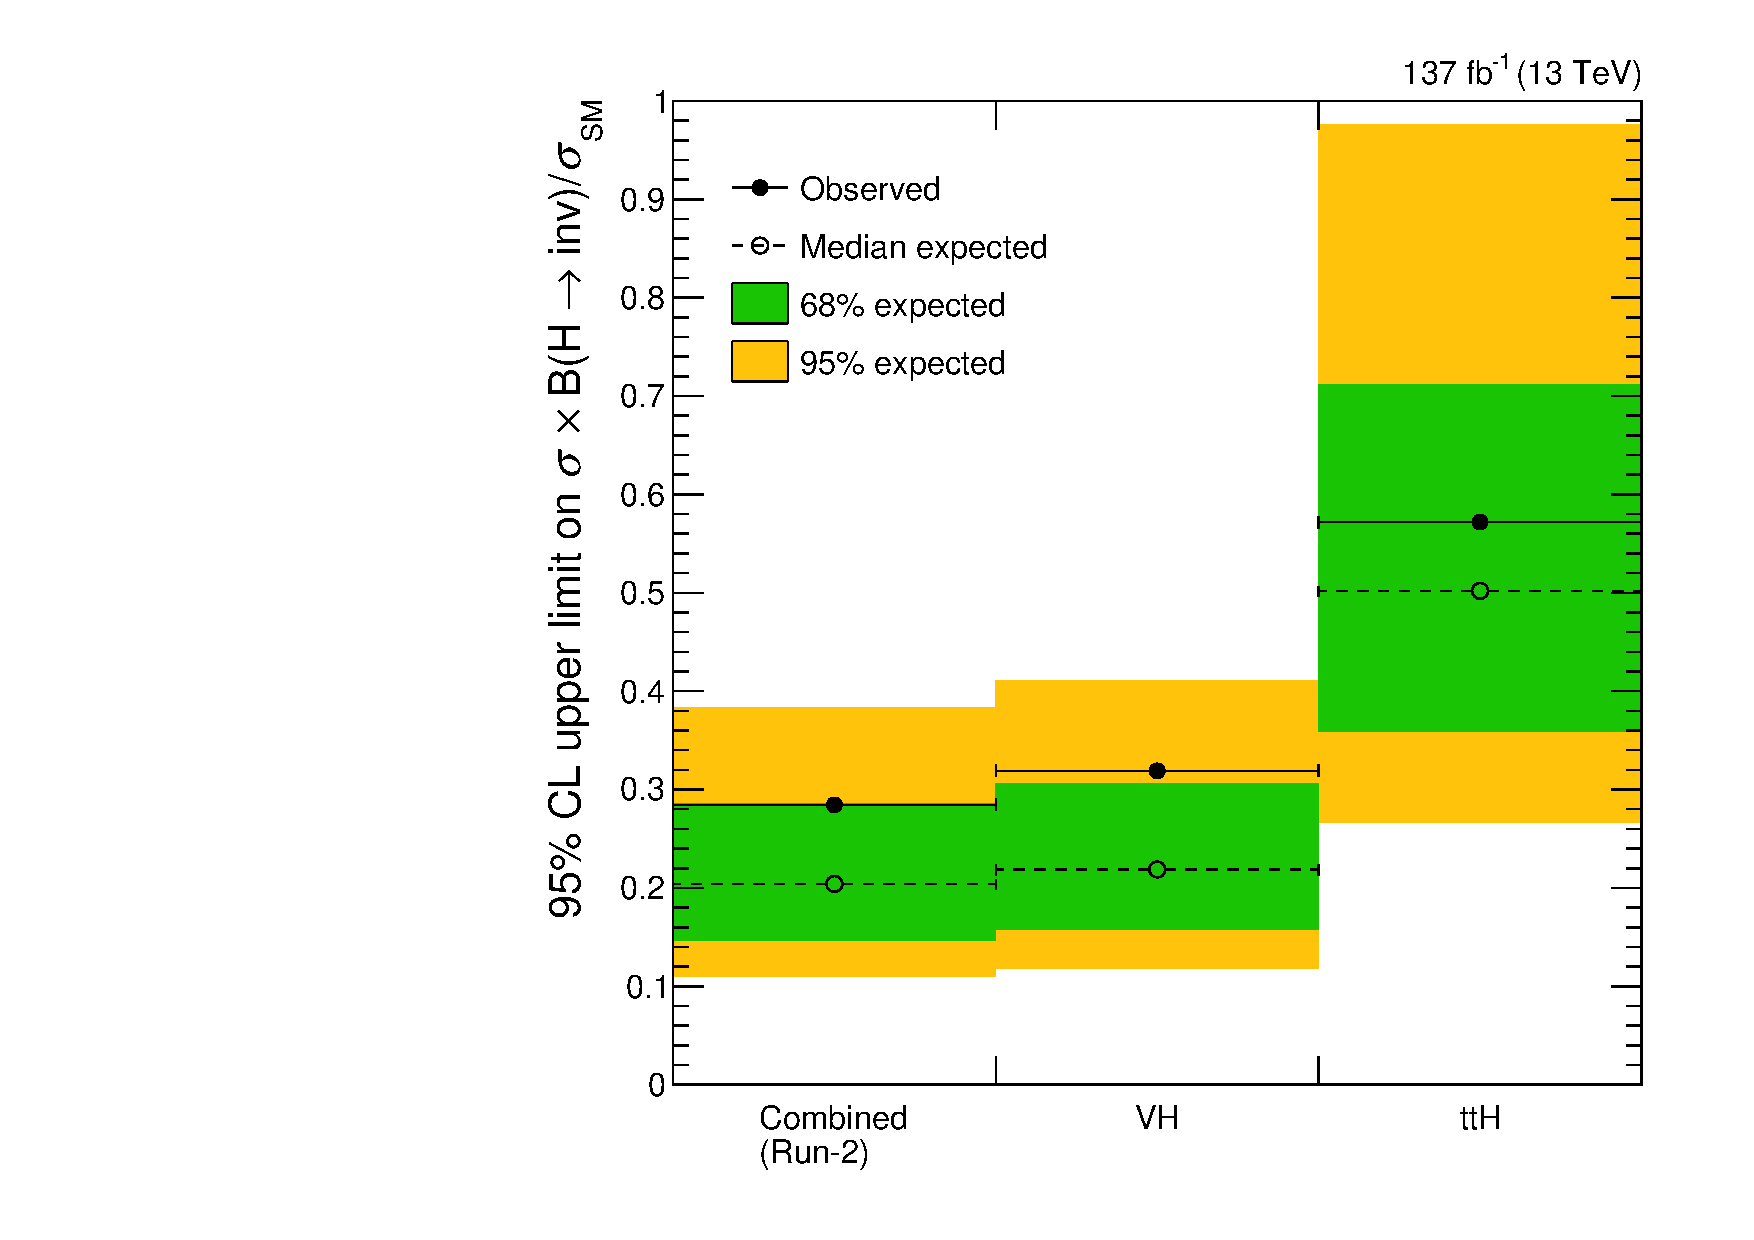
\includegraphics[width=\textwidth]{figures/limits/full_Run2/limit_Run2_comb_per_cat.pdf}
        \caption{Limit -- Run-2}
    \end{subfigure}
    \hspace{0.05\textwidth}
    \begin{subfigure}[b]{0.45\textwidth}
        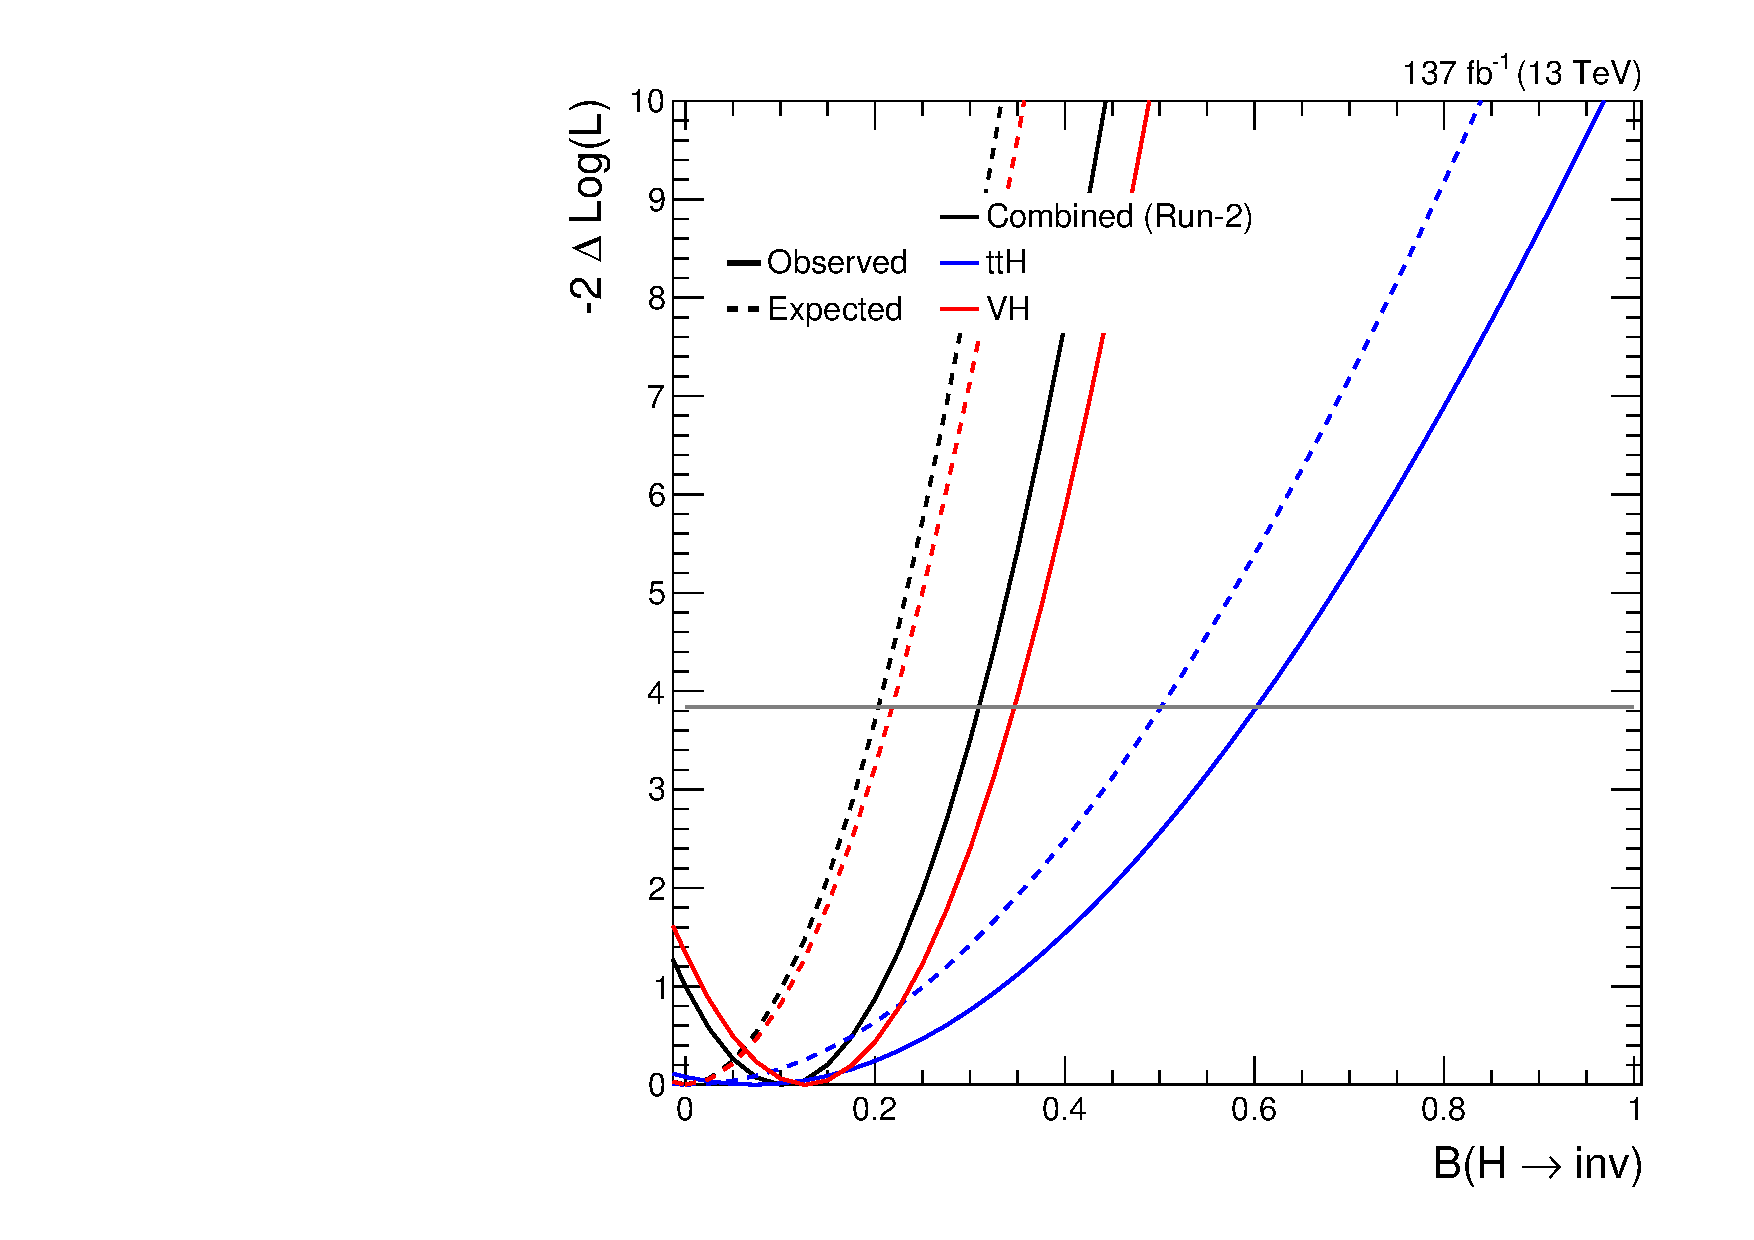
\includegraphics[width=\textwidth]{figures/likelihood_scan/profile_likelihood_scan_Run2_per_cat.pdf}
        \caption{Profile likelihood -- Run-2}
    \end{subfigure}
    \caption[Observed and expected 95\,\% CL upper limit on the Higgs boson to invisible state branching fraction $\BRof{\higgstoinv}$ and the corresponding profile likelihood ratio as a function of it, for both the individual categories, as well as the combination of them, for the full Run-2 dataset]{Observed and expected 95\,\% CL upper limit on the Higgs boson to invisible state branching fraction $\BRof{\higgstoinv}$ (left) and the corresponding profile likelihood ratio as a function of it (right), for both the individual categories, as well as the combination of them, for the full Run-2 dataset. The \acrlong{sm} Higgs boson with its associated mass and production cross section are assumed.}
    \label{fig:htoinv_limit_likelihood_Run2_per_cat}
\end{figure}

% Expected limits and likelihoods only, for Scenario 5. All limit and likelihood plots from 13th August

\begin{table}[htbp]
    \centering
    \begin{tabular}{ccccc}
        \hline\hline
        Dataset & \ttH & \VH & \ggH & Combined\\\hline
        \multirow{2}{*}{2016} & X (obs.) & X (obs.) & X (obs.) & X (obs.) \\
        & 69\,\% (exp.) & 43\,\% (exp.) & 48\,\% (exp.) & 29\,\% (exp.) \\\hline
        \multirow{2}{*}{2017} & X (obs.) & X (obs.) & X (obs.) & X (obs.) \\
        & 65\,\% (exp.) & 40\,\% (exp.) & 53\,\% (exp.) & 29\,\% (exp.) \\\hline
        \multirow{2}{*}{2018} & X (obs.) & X (obs.) & X (obs.) & X (obs.) \\
        & 62\,\% (exp.) & 36\,\% (exp.) & 34\,\% (exp.) & 23\,\% (exp.) \\\hline
        \multirow{2}{*}{Run-2} & X (obs.) & X (obs.) & X (obs.) & \textbf{X (obs.)} \\
        & 40\,\% (exp.) & 24\,\% (exp.) & 27\,\% (exp.) & \textbf{16\,\% (exp.)} \\\hline\hline
    \end{tabular}
    \caption{Observed and expected upper limits on $\BRof{\higgstoinv}$ for each category and dataset in the analysis.}
    \label{tab:hinv_limits}
\end{table}
